\documentclass{amsart}

% Commands for marginal notes
\usepackage[draft]{say}
\newcommand{\sayD}[1]{\say[D]{#1}}
\newcommand{\sayT}[1]{\say[T]{#1}}

\usepackage{amsmath,amssymb,latexsym,color}
\usepackage[bookmarks=true,colorlinks=true, linkcolor=blue, citecolor=cyan]{hyperref}
\usepackage{tikz}
\usepackage{pgflibraryarrows}
\usepackage{pgflibrarysnakes}
\usetikzlibrary{fit}
\usepackage[margin=1in,marginparwidth=0.8in, marginparsep=0.1in]{geometry}
\usepackage{extarrows}
\usepackage{verbatim}
\input xy
\xyoption{all}

%\usepackage[marginal]{showlabels}

\newtheorem{theorem}{Theorem}[section]
\newtheorem{claim}[theorem]{Claim}
\newtheorem{corollary}[theorem]{Corollary}
\newtheorem{definition}[theorem]{Definition}
\newtheorem{lemma}[theorem]{Lemma}
\newtheorem{question}[theorem]{Question}
\newtheorem{proposition}[theorem]{Proposition}
\newtheorem{remark}[theorem]{Remark}
\newtheorem{example}[theorem]{Example}

\newcommand{\bfe}{\mathbf{e}}
\newcommand{\bff}{\mathbf{f}}
\newcommand{\bfg}{\mathbf{g}}
\newcommand{\bfi}{\mathbf{i}}
\newcommand{\bfh}{\mathbf{h}}
\newcommand{\tbfe}{{\tilde\bfe}}
\newcommand{\tbff}{{\tilde\bff}}
\newcommand{\tbfg}{{\tilde\bfg}}
\newcommand{\tbfh}{{\tilde\bfh}}
\newcommand{\C}{\mathbb{C}}
\newcommand{\cC}{\mathcal{C}}
\newcommand{\cG}{\mathcal{G}}
\newcommand{\cP}{\mathcal{P}}
\newcommand{\ui}{\underline i}
\newcommand{\uj}{\underline j}
\newcommand\udim{{\underline{\dim}\, }}
\newcommand{\pt}{\mathrm{pt}}
\newcommand{\Rep}{\mathrm{Rep}}
\newcommand{\rep}{\operatorname{rep}}
\newcommand{\Gr}{\mathrm{Gr}}
\newcommand{\GL}{\mathrm{GL}}
\newcommand{\Ind}{\mathrm{Ind}}
\renewcommand{\AA}{\mathbb{A}}
\newcommand{\CC}{\mathbb{C}}
\newcommand{\kk}{\Bbbk}
\newcommand{\ZZ}{\mathbb{Z}}
\newcommand{\NN}{\mathbb{N}}
\newcommand{\rk}{\mathrm{rk}}
\newcommand{\Ext}{\operatorname{Ext}}
\newcommand{\Hom}{\operatorname{Hom}}
\newcommand{\im}{\operatorname{im}}
\newcommand{\codim}{\operatorname{codim}}
\newcommand{\into}{\hookrightarrow}
\newcommand{\onto}{\to\!\!\!\!\!\to}
\newcommand{\ses}[3]{0\rightarrow #1\rightarrow #2\rightarrow#3\rightarrow 0}
\newcommand{\sesm}[4]{0\rightarrow #1\rightarrow #2\xrightarrow{#4}#3\rightarrow 0}
\newcommand{\Sc}[2]{\langle #1,#2\rangle}
\newcommand{\spn}{\operatorname{span}}
\setcounter{MaxMatrixCols}{20}
\newcommand{\vs}{\vspace{0.2cm}}
\hyphenation{endo-functors}

\title{Cell Decompositions for Rank Two Quiver Grassmannians}

\author{Dylan Rupel}
\author{Thorsten Weist}

\begin{document}
\begin{abstract}
  We prove that all quiver Grassmannians for preprojective representations of a generalized Kronecker quiver admit a cell decomposition.  
  In the process, we introduce a class of regular representations which arise as quotients of consecutive preprojective representations.
  Cell decompositions for quiver Grassmannians of these ``truncated preprojectives'' are also established as well as for all indecomposable representations in their Auslander-Reiten components.
  We also provide a natural combinatorial labeling for these cells using compatible pairs in a maximal Dyck path. 
\end{abstract}

\setcounter{tocdepth}{2}

\maketitle

\tableofcontents
%%%%%%%%%%%%%%%%%%%%%%
\section{Introduction}
A cluster algebra is a subalgebra of a rational function field where generators are defined by an explicit recursion \cite{fomin-zelevinsky}.
Although the generators of the cluster algebra are given as rational functions they actually turn out to be Laurent polynomials.
These Laurent polynomial expressions for the cluster variables have been studied extensively and ultimately can be described using the representation theory of quivers \cite{caldero-chapoton,caldero-keller}: the cluster variables are generating functions for Euler characteristics of quiver Grassmannians.

For rank two cluster algebras, the Laurent expressions of cluster variables can also be computed using a certain Dyck path combinatorics \cite{lee-li-zelevinsky}.
The confluence of these results gives rise to a combinatorial construction for the Euler characteristics and counting polynomials of certain quiver Grassmannians.
Our main result is a geometric explanation for this correspondence by constructing a decomposition of these quiver Grassmannians into affine cells which are labeled by compatible pairs.

-something about compatible pairs and combinatorial construction of cluster variables\\
-statement of our results\\
-something about torus actions and the universal cover\\
-something about cell decompositions of quiver Grassmannians\\
-acknowledgements?\\


%%%%%%%%%%%%%%%%%%%%%%%%%%%%%%%%
\section{Quiver Covering Theory}
\label{sec:covering}

We refer to \cite{gab} for an introduction to covering theory.
Let $Q$ be an acyclic quiver with vertices $Q_0$ and arrows $Q_1$ which we denote by $\alpha:s(\alpha)\to t(\alpha)$.
A $\CC$-representation $X$ of $Q$ consists of a collection of $\CC$-vector spaces $X_i$ for $i\in Q_0$ and a collection of $\CC$-linear maps $X_\alpha:X_{s(\alpha)}\to X_{t(\alpha)}$ for $\alpha\in Q_1$.
Given $\CC$-representations $X$ and $Y$ of $Q$, a morphism $f:X\to Y$ is a collection of $\CC$-linear maps $f_i:X_i\to Y_i$ for $i\in Q_0$ satisfying $f_{t(\alpha)}\circ X_\alpha=Y_\alpha\circ f_{s(\alpha)}$ for each $\alpha\in Q_1$.
Write $\rep Q$ for the hereditary abelian category of $\C$-representations of $Q$.

Recall that, given $\CC$-representations $X$ and $Y$ of $Q$, any tuple of linear maps $(g_\alpha:X_{s(\alpha)}\to Y_{t(\alpha)})_{\alpha\in Q_1}$ defines a short exact sequence $\ses{Y}{Z}{X}$ with middle term given by the vector spaces $Z_i=X_i\oplus Y_i$ for $i\in Q_0$ and the linear maps $Z_\alpha=\begin{pmatrix} X_\alpha & 0 \\ g_\alpha & Y_\alpha \end{pmatrix}$ for $\alpha\in Q_1$. 
In general, considering the linear map  
\[d_{X,Y}:\bigoplus_{i\in Q_0}\Hom_\CC(X_i,Y_i)\to\bigoplus_{\alpha\in Q_1}\Hom_\CC(X_{s(\alpha)},Y_{t(\alpha)}),\qquad (f_i)_{i\in Q_0}\mapsto(f_{t(\alpha)}\circ X_\alpha-Y_\alpha\circ f_{s(\alpha)})_{\alpha\in Q_1},\]
we have $\mathrm{ker}(d_{X,Y})=\Hom_Q(X,Y)$ and $\mathrm{coker}(d_{X,Y})=\Ext_Q(X,Y)$.

Let $W_Q$ be the free non-abelian group generated by $Q_1$.  
Write $A_Q\cong \ZZ^{Q_1}$ for the free abelian group generated by $Q_1$ and denote by $e_\alpha\in A_Q$ the generator corresponding to $\alpha\in Q_1$. 
\begin{definition}
  The \emph{universal abelian covering quiver} $\hat Q$ of $Q$ has vertices $\hat Q_0=Q_0\times A_Q$ and arrows $\hat Q_1=Q_1\times A_Q$, where $(\alpha,\chi):\big(s(\alpha),\chi\big)\to\big(t(\alpha),\chi+e_\alpha\big)$ for $\alpha\in Q_1$ and $\chi\in A_Q$.
  Write $F_Q:\rep \hat Q\to\rep Q$ for the natural functor. 

  The \emph{universal covering quiver} $\widetilde Q$ of $Q$ has vertices $\widetilde Q_0=Q_0\times W_Q$ and arrows $\widetilde Q_1=Q_1\times W_Q$, where $(\alpha,w):\big(s(\alpha),w\big)\to\big(t(\alpha),w\alpha\big)$\sayD{Should we write $\alpha w$ here so that arrows act of the left and compose as functions?} for $\alpha\in Q_1$ and $w\in W_Q$.
  Write $G_Q:\rep\widetilde Q\to\rep Q$ for the natural functor. 

  We say that a representation $X\in\rep Q$ can be \emph{lifted} to $\hat Q$ (resp. $\widetilde Q$) if there exists a representation $\hat X\in\rep \hat Q$ (resp. $\widetilde X\in\rep \widetilde Q$) such that $F_Q\hat X=X$ (resp. $G_Q \widetilde X=X$).
\end{definition}

Note that in our definition every covering quiver has infinitely many connected components, but each of its connected components is a covering in the sense of \cite{gab}.
As indecomposable representations live on one of these components this distinction will be irrelevant.
Note that the natural surjection $W_Q\onto A_Q$ induces a functor $H_Q:\rep \widetilde Q\to\rep \hat Q$.
In addition, observe that every connected component of the universal covering quiver of the universal abelian covering quiver is isomorphic to a connected component of the universal covering quiver of the original quiver.

\begin{lemma}
  Every preprojective and preinjective representation of $Q$ can be lifted to $\hat Q$ and to $\widetilde Q$.
\end{lemma}
\begin{proof}
  This statement is clear for the simple representations $S_i$, $i\in Q_0$.
  Now every preprojective or preinjective representation of $Q$ can be obtained by applying a sequence of BGP-reflections \cite{bgp} to a simple representation $S'_j$ of a quiver $Q'$ whose underlying graph is the same as the one for $Q$.
  Applying a BGP-reflection to a fixed vertex $i$ of $Q$ corresponds to applying BGP-reflections to all vertices $(i,\chi)\in\hat Q_0$, where $\chi$ runs through all $\chi\in A_Q$ (resp. to all $(i,w)\in \tilde Q_0$ with $w\in W_Q$).
  This gives the claim.
\end{proof}

The functor $F_Q$ induces a map $F_Q:\ZZ^{\hat Q_1}\to \ZZ^{Q_1}$.
We say that a dimension vector $\hat \bfe$ of $\hat Q$ is \emph{compatible} with $\bfe$ if $F_Q(\hat\bfe)=\bfe$.
The group $A_Q$ acts on $\hat Q$ via translation, this induces actions of $A_Q$ on $\rep\hat Q$ and on $\ZZ^{\hat Q_1}$.
We say two representation (resp. dimension vectors) are \emph{equivalent} if they can be related by the action of $A_Q$.
The analogous observation can also be made for $\widetilde Q$.
If $X$ is a representation of $\hat Q$ (resp. $\widetilde Q$), we denote by $X_\chi$ (resp. $X_w$) the representation obtained via translation by $\chi\in A_Q$ (resp. $w\in W_Q$).  

As $F_Q$ and $G_Q$ are covering functors when restricting to one connected component, we obtain the following result from \cite{gab}.
\sayD{Specific reference needed?}
\begin{theorem}
  \label{covering}
  The functors $F_Q$ and $G_Q$ preserve indecomposability.
  Moreover, for all representations $\hat X,\hat Y \in\rep(\hat Q)$, we have 
  \[\Hom_Q(F_Q\hat X, F_Q\hat Y)\cong \bigoplus_{\chi\in A_Q}\Hom_{\hat Q}(\hat X_\chi,\hat Y)\cong\bigoplus_{\chi\in A_Q}\Hom_{\hat Q}(\hat X,\hat Y_\chi).\]
  Analogous isomorphisms exist when replacing $\Hom$ by $\Ext$ and/or $\rep \hat Q$ by $\rep\widetilde Q$.
\end{theorem}


%%%%%%%%%%%%%%%%%%%%%%%%%%%%%%%%%%%%%%%%%
\section{Representation Theory of $K(n)$}\label{sec:RepK(n)}

Fix $n\ge3$. Denote by $K(n)$ the \emph{$n$-Kronecker quiver} $1\stackrel{n}{\longleftarrow}2$ with vertices $K_0(n)=\{1,2\}$ and $n$ arrows from vertex $2$ to vertex $1$. 
The category $\rep K(n)$ of finite-dimensional representations of $K(n)$ is equivalent to the category of modules over the path algebra $A(n)$ of $K(n)$.
As a $\CC$-vector space, the path algebra $A(n)$ can be written as $A_0\oplus A_1$, where 
\begin{itemize}
  \item $A_0=\CC e_1\oplus \CC e_2$ is a two-dimensional semisimple algebra with orthogonal idempotents $e_1$ and $e_2$;
  \item $A_1=\bigoplus_{i=1}^n \CC\alpha_i$ is the $A_0$-bimodule spanned by the arrows of $K(n)$, that is $e_k\alpha_ie_\ell=\delta_{k1}\delta_{\ell2}\alpha_i$ for $1\le i\le n$ and $k,\ell\in\{1,2\}$.
\end{itemize}

Write $\Sigma_1$ and $\Sigma_2$ for the BGP-reflection functors of $K(n)$ \cite{bgp}. 
We use the same symbols $\Sigma_1$, $\Sigma_2$ for the BGP-reflection functors of $K(n)^{op}$, this should not lead to any confusion. 
Then each endofunctor $\Sigma_i^2$ is naturally isomorphic to the identity map on the full subcategory $\rep_{\langle i\rangle} K(n)\subset \rep K(n)$ whose objects are those representations of $K(n)$ which do not contain the simple $S_i$ as a direct summand.
In particular, $\Sigma_i$ gives an exact equivalence of categories $\Sigma_i:\rep_{\langle i\rangle} K(n)\to\rep_{\langle i\rangle} K(n)^{op}$.
Also, following \cite{brenner-butler}, the Auslander-Reiten translation $\tau:\rep K(n)\to\rep K(n)$ may be identified with the functor $\Sigma_2\Sigma_1$.

Define Chebyshev polynomials $u_k$ for $k\in\ZZ$ by the recursion $u_0=0$, $u_1=1$, $u_{k+1}=nu_k-u_{k-1}$.
The following is well-known.
\begin{theorem}
  \label{th:rigids}
  For each $m\ge1$, there exist unique (up to isomorphism) indecomposable rigid representations $P_m$ and $I_m$ of $K(n)$ with dimension vectors $(u_m,u_{m-1})$ and $(u_{m-1},u_m)$ respectively. 
  Moreover, any rigid representation of $K(n)$ is isomorphic to one of the form $P_m^{a_1}\oplus P_{m+1}^{a_2}$ or $I_m^{a_1}\oplus I_{m+1}^{a_2}$ for some $m\ge1$ and some $a_1,a_2\ge0$.
\end{theorem}
The representations $P_m$ are called the \emph{preprojective} representations of $K(n)$ and the representations $I_m$ are called \emph{preinjective}.
\begin{remark}
  \label{rem:reflection recursion}
  We may identify the quiver $K(n)$ with $K(n)^{op}$ by interchanging the vertex labels.
  This induces an isomorphism of categories $\rep K(n)\cong\rep K(n)^{op}$ which we write as $M\mapsto M^\sigma$.
  Note that $\Sigma_1(M^\sigma)=(\Sigma_2 M)^\sigma$ and $\Sigma_2(M^\sigma)=(\Sigma_1 M)^\sigma$.
  \begin{enumerate}
    \item The preprojective and preinjective representations satisfy the following recursions using the reflection functors:
      \[P_1=S_1,\quad P_m^\sigma=\Sigma_2 P_{m-1},\quad I_1=S_2,\quad I_m^\sigma=\Sigma_1 I_{m-1}\]
      for $m\ge2$.
      In particular, we have $P_{m-1}=\tau P_{m+1}$ and $I_{m+1}=\tau I_{m-1}$ for $m\ge2$.
    \item If $\ses{M}{B}{N}$ is a short exact sequence such that no direct summand of $M$, $B$, nor $N$ is preinjective, then the sequences $\ses{(\Sigma_1\Sigma_2)^nM}{(\Sigma_1\Sigma_2)^nB}{(\Sigma_1\Sigma_2)^nN}$ and $\ses{\Sigma_2(\Sigma_1\Sigma_2)^nM}{\Sigma_2(\Sigma_1\Sigma_2)^nB}{\Sigma_2(\Sigma_1\Sigma_2)^nN}$ are exact for any $n\ge0$ and none of these representations contain preinjective direct summands.
      %Without the assumption on the direct summands, it is not clear that short exact sequences are preserved.
      %This is because $\Sigma_2 S_2=0$.
  \end{enumerate}
\end{remark}
We will see that the indecomposable representations of dimension $d(m,r):=\dim P_{m+1}-r\dim P_m$ with $0\leq r\leq n-1$ play an important role as they appear as quotients of morphisms between preprojective representations.
For a dimension vector $d\in\NN^{Q_0}$, write $R_d(K(n))$ for the affine space of representations of dimension $d$.
\begin{proposition}
  \label{pro:indecomposables}
  Let $m\geq 1$ and $0\le r\le n-1$.
  The following hold:
  %\sayD{Move the first two of these into section~\ref{sec:truncated preprojectives}?}
  \begin{enumerate}
    \item The isomorphism classes of indecomposable representations of dimension $d(m,r)$ are in one-to-one correspondence with points of $\Gr_{n-r}(\CC^n)$.
    \item The set of indecomposable representations of dimension $d(m,r)$ is given by a non-empty open subset of $R_{d(m,r)}(K(n))$. 
   % \item The action of $\GL_n(\CC)$ is transitive on $\mathrm{Ind}(K(n),\alpha(m,r))$.
  \end{enumerate}
\end{proposition}
\begin{proof}
  As the reflection functors $\Sigma_1,\,\Sigma_2$ preserve indecomposability and $\Sigma_2(d(m,r))^\sigma=d(m+1,r)$, it suffices to prove the first statement for $m=1$.
  Then we have $d(m,r)=(l,1)$ for $l:=n-r$.
  This means that $X\in R_{d(m,r)}(K(n))$ can be represented by a matrix $M_X\in\CC^{l\times n}$, where the $i^{\mathrm{th}}$ column stands for $X_{\alpha_i}$.
  Now $X$ is indecomposable if and only if $\rk(M_X)=l$.
  Indeed, $X$ admits a summand isomorphic to $S_1^k$ exactly when $\rk(M_X)=l-k$.

  This shows that the indecomposable representations in $R_{(l,1)}(K(n))$ are in one-to-one correspondence with $l\times n$ matrices of maximal rank.
  Thus we may associate to each such representation $X$ a subspace of $\CC^n$ of dimension~$l$ spanned by the row vectors of the corresponding matrix $M_X$.
  Now it is straightforward to check that the $\GL_{d(m,r)}=\GL_l(\CC)\times\CC^\ast$-action on $R_{d(m,r)}(K(n))$ corresponds to the base change action of $\GL_l(\CC)$ on the set of these subspaces.
  This shows the first statement.

  It is easy to see that $(l,1)$ is a Schur root since all indecomposable representations with this dimension vector have trivial endomorphism ring.
  Thus the roots $d(m,r)$ are also Schur roots.
  \sayD{This can also be seen as a consequence of Corollary~\ref{cor:indecomposable truncated}, would it be better if we reorganize?}
  It follows that the set of indecomposable representations with trivial endomorphism ring form a dense open subset of $R_{d(m,r)}(K(n))$, see for example \cite[Theorem 2.2]{sch}.
  This shows the second statement.

%For $m=1$, the action of $\GL_n(\CC)$ on $\Gr_d(\CC^n)$ is transitive which shows that it is transitive on $\Ind_\alpha(K(n))$. As the reflection functors preserve indecomposability and isomorphism classes, by Lemma \ref{compatibleGSigma}, for every $g\in\GL_n(\CC)$, we obtain a commutative diagram
%\[\xymatrix{\Ind(K(n),\alpha(m,r))\ar[r]^{\Sigma_2}\ar[d]^{g^{-T}}&\Ind(K(n),\alpha(m+1,r))\ar[d]^g\\
%\Ind(K(n),\alpha(m,r))\ar[r]^{\Sigma_2}&\Ind(K(n),\alpha(m+1,r))}\]
%As the $\GL_n(\CC)$-action is transitive on the left hand side, this implies that it is also transitive on the right hand side.
\end{proof}
\begin{remark}
  There is a more elegant way to prove Proposition \ref{pro:indecomposables} using the notion of stability and moduli spaces.
  Actually, fixing the standard stability induced by the linear form $\Theta(\alpha)=\alpha_2$, it can be shown that all indecomposables are stable and that the moduli space of stable representations is in fact $\Gr_l(\CC^n)$.
  We opted for the proof above because the notion of stability would only be used at this point and we wanted to keep the exposition as simple as possible. 
\end{remark}

Set $H_m:=\Hom(P_m,P_{m+1})$ for $m\ge1$. %and define an action of $GL_n(\CC)$ on $H_m$ by $g.\theta:=\phi_{m+1,g}^{-1}\circ\theta^g\circ\phi_{m,g}$.
%Note that the first $\theta$ here represents an element of $H_m$ while the second $\theta^g$ represents the corresponding element of $H_m^g:=\Hom(g.P_m,g.P_{m+1})$ from Lemma~\ref{le:hom equivariance}.
Write $\Gr(H_m)$ for the \emph{total Grassmannian} of $H_m$ whose elements are nontrivial proper subspaces $V\subset H_m$.
Some results below remain true if we allow $H_m$ or $0$ as elements of $\Gr(H_m)$, but not all, so for uniformity of exposition we omit these possibilities.
%Lemma~\ref{le:hom equivariance} gives an identification of $\Gr(H_m)$ with $\Gr(H_m^g)$ and we write $V\mapsto V^g$ for this correspondence.
For $1\le r\le n-1$, let $\Gr_r(H_m)\subset \Gr(H_m)$ be the subvariety of $r$-dimensional subspaces of $H_m$.

For each $m\ge2$, there is an Auslander-Reiten sequence (cf.\ \cite[Section V]{ars})
\begin{equation}
  \label{eq:AR sequence}
  0\longrightarrow P_{m-1}\stackrel{\iota_{m-1}}{\longrightarrow} P_m\otimes H_m\stackrel{ev}{\longrightarrow} P_{m+1}\longrightarrow 0,
\end{equation}
where the right-hand morphism is the natural evaluation map.

\begin{lemma}
  \label{le:injective evaluation maps}
  For any $V\in \Gr(H_m)$, $m\geq 1$, the natural evaluation map $ev_V:P_m\otimes V\to P_{m+1}$ is injective.
\end{lemma}
%%%%%%%%%%%%%%%%%%%
% needs polishing %
%%%%%%%%%%%%%%%%%%%
\begin{proof}\sayT{Maybe we can shorten the proof. I don't see a  proof which does not use reflection functors at the moment.}
  As $\Ext(P_m\otimes V,P_{m-1})=0$ and $\Hom(P_1,I_1)=0$, we obtain a commutative diagram 
  \[\xymatrix{0 \ar[r] & P_{m-1}\ar@{=}[d]\ar[r] &P_{m-1}\oplus P_m\otimes V \ar@{}[dr]|(.7){\lrcorner} \ar[r]\ar[d]_{(\iota_{m-1},\mathrm{id}_{P_m}\otimes \iota_V)} &P_{m}\otimes V \ar[r]\ar_{ev_V}[d] & 0 \ar[d]\\ 0 \ar[r] & P_{m-1}\ar[r]^{\iota_{m-1}} & P_m\otimes H_m \ar[r]^{ev} &P_{m+1} \ar[r] & I_{2-m}\ar[r]&0}\]
  in which we set $P_0=0$ and $I_l=0$ for $l\leq 0$.
  Since $\mathrm{id}_{P_1}\otimes \iota_V$ is injective, the snake lemma shows that $\ker ev_V=0$ for $m=1$ and thus $ev_V$ is injective in this case.
  
  In view of Remark~\ref{rem:reflection recursion}, it is enough for the case $m>1$ to show that the cokernel of $ev_V$ does not have a preinjective direct summand when $m=1$.
  Clearly the cokernel of $\mathrm{id}_{P_1}\otimes \iota_V$ is isomorphic to $P_1\otimes H_1/V$.
  Thus we obtain the following commutative diagram induced by the cokernels of the above vertical maps, note that the vertical maps below are surjective:
  \[\xymatrix{0 \ar[r]  & P_1\otimes H_1 \ar[d]\ar[r]^{ev} &P_{2}\ar[d] \ar[r] & I_{1}\ar@{=}[d]\ar[r]&0\\ 0\ar[r] & P_1\otimes H_1/V \ar[r] &K\ar[r]& I_{1}\ar[r]&0.}\]

  We need to show that $K$ has no preinjective direct summand.
  As $\Hom(P_2,P_1)=0$, the representation $K$ has no direct summand which is isomorphic to $P_1=S_1$.
  But this already shows that $K$ is indecomposable as $\udim K=(\dim H_1/V,1)$.
  Since $V$ is a proper subspace of $H_1$, $\udim K$ is not the dimension vector of a preinjective representation and the claim follows.
\end{proof}

In what follows we will not distinguish between $P_m\otimes V$ and its image under $ev_V$.

\subsection{Truncated Preprojectives}
\label{sec:truncated preprojectives}
Following Lemma~\ref{le:injective evaluation maps}, we define the following.
\begin{definition}
  For $V\in \Gr(H_m)$, define the \emph{truncated preprojective} $P_{m+1}^V$ to be the cokernel of the map $ev_V:P_m\otimes V\to P_{m+1}$, i.e.\ we have a short exact sequence
  \begin{equation}
    \label{eq:truncated preprojectives}
    0\longrightarrow P_m\otimes V\stackrel{ev_V}{\longrightarrow} P_{m+1}\stackrel{\pi_V}{\longrightarrow} P_{m+1}^V\longrightarrow 0.
  \end{equation}
\end{definition}
\begin{remark}
  It will be convenient to also set $P_{m+1}^0=P_{m+1}$, observe that this notation is consistent with taking $V=0$ in the sequence \eqref{eq:truncated preprojectives}.
\end{remark}

\begin{lemma}
  \label{le:truncated homomorphisms}
  For $V\in \Gr(H_m)$, $m\ge1$, we have $\Hom(P_m,P_{m+1}^V)\cong H_m/V$ and $\Ext(P_m,P_{m+1}^V)=0$.
\end{lemma}
\begin{proof}
  Applying the functor $\Hom(P_m,-)$ to the sequence \eqref{eq:truncated preprojectives} gives an exact sequence
  \[\xymatrix{0 \ar[r] & \Hom(P_m,P_m\otimes V) \ar[r] & \Hom(P_m,P_{m+1}) \ar[r] & \Hom(P_m,P_{m+1}^V) \ar[r] & 0}\]
  and a surjective map
  \[\Ext(P_m,P_{m+1})\onto\Ext(P_m,P_{m+1}^V).\]
  But there is a natural isomorphism $\Hom(P_m,P_m\otimes V)\cong V$ and the first claim follows.
  The final claim follows from Remark~\ref{rem:reflection recursion}.
\end{proof}

\begin{lemma}
  \label{le:unique preprojective morphism}
  For $V\in \Gr(H_m)$, $m\ge1$, the space $\Hom(P_{m+1},P_{m+1}^V)$ is one-dimensional spanned by the natural projection $\pi_V:P_{m+1}\to P_{m+1}^V$.
  Moreover, $\Ext(P_{m+1},P_{m+1}^V)=0$.
\end{lemma}
\begin{proof}
  Applying the functor $\Hom(P_{m+1},-)$ to the sequence \eqref{eq:truncated preprojectives}, we obtain an isomorphism 
  \[\Hom(P_{m+1},P_{m+1})\cong\Hom(P_{m+1},P_{m+1}^V)\]
  and a surjective map
  \[\Ext(P_{m+1},P_{m+1})\onto\Ext(P_{m+1},P_{m+1}^V).\]
  The identity map on $P_{m+1}$ is taken to the projection $\pi_V:P_{m+1}\to P_{m+1}^V$ under the isomorphism.
  The rigidity of $P_{m+1}$ gives the final claim.
\end{proof}

\begin{lemma}
  \label{le:unique morphisms}
  Consider $V,W\in \Gr(H_m)$, $m\ge1$.
  \begin{enumerate}
    \item There exists a morphism $P_{m+1}^W\to P_{m+1}^V$ if and only if $W\subset V$ and this morphism is unique (up to scalars) when it exists.
    \item For $W\subset V$, we have $\Ext(P_{m+1}^W,P_{m+1}^V)\cong W^*\otimes(H_m/V)$.
  \end{enumerate}
\end{lemma}
\begin{proof}
  We apply the functor $\Hom(-,P_{m+1}^V)$ to the sequence \eqref{eq:truncated preprojectives} for $W$ to get an exact sequence
  \[0\longrightarrow \Hom(P_{m+1}^W,P_{m+1}^V)\longrightarrow \Hom(P_{m+1},P_{m+1}^V)\stackrel{-\circ ev_W}{\longrightarrow} \Hom(P_m\otimes W,P_{m+1}^V)\longrightarrow \Ext(P_{m+1}^W,P_{m+1}^V)\longrightarrow 0.\]
  But the space $\Hom(P_{m+1},P_{m+1}^V)$ is one-dimensional and thus $\Hom(P_{m+1}^W,P_{m+1}^V)$ is nonzero if and only if the right hand morphism of the above sequence is zero.
  But this occurs exactly when the image of $ev_W:P_m\otimes W\to P_{m+1}$ is contained in the kernel of $\pi_V$, i.e.\ in the image of $ev_V:P_m\otimes V\to P_{m+1}$, and this occurs if and only if $W\subset V$. 
  In this case, there are isomorphisms
  \[\Ext(P_{m+1}^W,P_{m+1}^V)\cong\Hom(P_m\otimes W,P_{m+1}^V)\cong W^*\otimes H_m/V,\]
  where the last isomorphism is immediate from Lemma~\ref{le:truncated homomorphisms}.
\end{proof}

\begin{remark}
  The total Grassmannian $\Gr(H_m)$ is naturally a poset under inclusion.
  This structure gives rise to a $\CC$-linear category $\CC \Gr(H_m)$ with objects the elements of $\Gr(H_m)$ and at most one morphism (up to scalars) between any two objects.
  Write $\cP_{m+1}$ for the full subcategory of $\rep K(n)$ with objects the truncated preprojectives $P_{m+1}^V$ for $V\in \Gr(H_m)$.
  By Lemma~\ref{le:unique morphisms}(1), the functor $V\mapsto P_{m+1}^V$ gives an isomorphism of categories $\CC \Gr(H_m)\cong\cP_{m+1}$.
\end{remark}

\begin{corollary}
  \label{cor:indecomposable truncated} 
  For $V\in \Gr(H_m)$, $m\ge1$, the truncated preprojective $P_{m+1}^V$ is indecomposable.
  Moreover, every indecomposable of dimension $\udim P_{m+1}^V$ is truncated preprojective.
\end{corollary}
\begin{proof}
  By Lemma~\ref{le:unique morphisms}, the endomorphism ring of $P_{m+1}^V$ is one-dimensional and so $P_{m+1}^V$ must be indecomposable.
  The second part follows from Proposition \ref{pro:indecomposables} together with Lemma \ref{le:unique morphisms}.
\end{proof}

\begin{lemma}
  \label{le:basic homological properties}
  For $V\in\Gr(H_m)$, $m\ge1$, we have $\Hom(P_{m+1}^V,P_\ell)=0=\Ext(P_\ell,P_{m+1}^V)$ for all $\ell\ge1$.
\end{lemma}
\begin{proof}
  Recall that $\Hom(X,P_\ell)\ne0$ (resp. $\Ext(P_\ell,X)\ne0$) for some $\ell\ge1$ implies all indecomposable summands of $X$ are preprojectives of the form $P_r$ with $1\le r\le\ell$ (resp. $1\le r\le\ell-2$).
  However, $P_{m+1}^V$ cannot be preprojective as it is not rigid by Lemma~\ref{le:unique morphisms}.
  %Note that $\udim P_{m+1}^V <\udim P_{m+1}$, but $\udim P_r\geq \udim P_{m+1}$ if $\Hom(P_{m+1},P_r)\neq 0$.
\end{proof}

\begin{lemma}
  For $V\in\Gr(H_m)$, $m\ge1$, the representation $\Sigma_2(P_{m+1}^V)^\sigma$ is also truncated preprojective.
\end{lemma}
\begin{proof}
  Apply the functor $\Sigma_2(-)^\sigma$ to the sequence \eqref{eq:truncated preprojectives}.
\end{proof}

\begin{lemma}
  \label{le:unique truncated extension}
  For $V\in \Gr(H_m)$, $m\ge2$, the space $\Ext(P_{m+1}^V,P_{m-1})$ is one-dimensional and spanned by the extension
  \begin{equation}
    \label{eq:unique extension}
    \xymatrix{0 \ar[r] & P_{m-1} \ar[r]^(.375){\kappa_V} & P_m\otimes(H_m/V) \ar[r]^(.625){ev} & P_{m+1}^V \ar[r] & 0}.
  \end{equation}
\end{lemma}
\begin{proof}
  Applying the functor $\Hom(-,P_{m-1})$ to the sequence \eqref{eq:truncated preprojectives} gives an isomorphism $\Ext(P_{m+1}^V,P_{m-1})\cong\Ext(P_{m+1},P_{m-1})$ with a one-dimensional space.
  Writing $X$ for the unique extension of $P_{m+1}^V$ by $P_{m-1}$, this isomorphism gives rise to the following pullback diagram:
  \[\xymatrix{ & & 0 \ar[d] & 0\ar[d] & \\
    & & P_m\otimes V \ar@{=}[r]\ar[d] & P_m\otimes V\ar[d] & \\
    0 \ar[r] & P_{m-1} \ar@{=}[d]\ar[r]^(.425){\iota_{m-1}} & P_m\otimes H_m \ar[r]\ar[d]\ar@{}[dr]|(.7){\lrcorner} & P_{m+1} \ar[r]\ar[d] & 0\\
    0 \ar[r] & P_{m-1} \ar[r]^{\kappa_V} & X \ar[r]\ar[d] & P_{m+1}^V \ar[r]\ar[d] & 0\\
    & & 0 & 0 & }\]
  from which we immediately obtain the isomorphism $X\cong P_m\otimes(H_m/V)$.
\end{proof}

\begin{lemma}
  \label{le:preprojective homomorphism duality}
  The sequence \eqref{eq:AR sequence} gives rise to an isomorphism $H_m^*\cong H_{m-1}$.
\end{lemma}
\begin{proof}
  Define a map $H_m^*\to H_{m-1}$ by $\varphi\mapsto\bar{\varphi}:=(id\overline{\otimes}\varphi)\circ\iota_{m-1}$, in words $\bar{\varphi}$ acts on $x\in P_{m-1}$ by contracting with the second factor in $\iota_{m-1}(x)$ to give an element of $P_m$.
  Suppose $\varphi\in H_m^*$ is a nonzero functional on $H_m$ and let $V\subsetneq H_m$ denote the kernel of $\varphi$.
  Then $\bar{\varphi}=0\in H_{m-1}$ if and only if the image of $\iota_{m-1}$ is contained in $P_m\otimes V\subsetneq P_m\otimes H_m$.
  But then Lemma~\ref{le:injective evaluation maps} implies $ev\circ\iota_{m-1}=ev_V\circ\iota_{m-1}\ne0$, a contradiction.
  Thus the map $H_m^*\to H_{m-1}$, $\varphi\mapsto\bar{\varphi}$ must be injective and hence an isomorphism.
\end{proof}
\begin{remark}
  The set $\Gr(H_m)$ is naturally a poset and Lemma~\ref{le:preprojective homomorphism duality} gives an identification of the opposite poset $\Gr(H_m)^{op}\cong \Gr(H_m^*)$ with $\Gr(H_{m-1})$.
  We write $\bar{V}\subset H_{m-1}$ for the subspace corresponding to $V\subset H_m$ under this identification.
  Under the isomorphism of $H_{m-1}$ with $H_m^*$, we have $\bar{V}=(H_m/V)^*$.\sayT{more details?}
\end{remark}

\begin{corollary}
  \label{cor:truncated preprojective isomorphism}
  Suppose $V\in \Gr(H_m)$ has codimension-one in $H_m$.  Then $P_{m+1}^V\cong P_m^{\bar{V}}$.
\end{corollary}
\begin{proof}
  By Lemma~\ref{le:unique truncated extension}, we have the exact sequence
  \[\xymatrix{0 \ar[r] & P_{m-1} \ar[r]^(.35){\kappa_V} & P_m\otimes(H_m/V) \ar[r]^(.625){ev} & P_{m+1}^V \ar[r] & 0}.\]
  But $H_m/V$ is a one-dimensional vector space and so $P_m\otimes(H_m/V)\cong P_m$.
  Under this identification, the left hand morphism $\kappa_V$ in the sequence above identifies with a generator of $\bar{V}$ and thus $P_{m+1}^V\cong P_m^{\bar{V}}$.
\end{proof}

Following Remark~\ref{rem:reflection recursion}, the reflection functor $\Sigma_1$ provides a natural identification of $H_m$ with $H_{m-1}$ for $m\ge2$. 
Combining with Lemma~\ref{le:preprojective homomorphism duality} we obtain a natural isomorphism $H_m^*\cong H_m$ for $m\ge2$.
The next observation is essential for the results to follow.
\begin{proposition}
  For $V\in \Gr(H_m)$, $m\ge1$, we have $\bar{\bar{V}}=\tau V$.
\end{proposition}
\begin{proof}
  \sayD{Proof needed}\sayT{explain $\tau V$. Do we need this?}
  We show that $\bar{\bar{\varphi}}=\tau\varphi$ for $\varphi\in H_m$.
  Indeed, we have
  \[\bar{\bar{\varphi}}=(id\overline{\otimes}\bar{\varphi})\circ\iota_{m-2}=\Big(id\overline{\otimes}\big((id\overline{\otimes}\varphi)\circ\iota_{m-1}\big)\Big)\circ\iota_{m-2}.\]
\end{proof}

\begin{lemma}
  \label{le:truncated extensions}
  For $V\in \Gr(H_m)$, $m\ge1$, we have $\Ext(P_{m+1}^V,P_m)\cong V^*$, where each nontrivial extension naturally corresponds to a codimension 1 subspace $U\subset V$. 
  More precisely, each element of $\Ext(P_{m+1}^V,P_m)$ corresponds to an exact sequence
  \[\xymatrix{0 \ar[r] & P_m \ar[r] & P_{m+1}^U \ar[r] & P_{m+1}^V \ar[r] & 0},\]
where $U\subset V$ satisfies $\dim(V/U)=1$.
\end{lemma}
\begin{proof}
  Consider a nonzero map $\varphi\in V^*$ and set $U=\ker\varphi\subset V$.
  There is a natural isomorphism $V^*\cong\Hom(P_m\otimes V,P_m)$ which takes $\varphi$ to $id\overline{\otimes}\varphi$.
  This gives rise to the following commutative diagram:
  \[\xymatrix{ & 0 \ar[d] & 0 \ar[d] & & \\
    & P_m\otimes U \ar@{=}[r]\ar[d] & P_m\otimes U \ar[d] & & \\
    0 \ar[r] & P_m\otimes V \ar[d]^{id\overline{\otimes}\varphi}\ar[r]\ar@{}[dr]|(.7){\lrcorner}\ar@{}[dr]|(.3){\ulcorner} & P_{m+1} \ar[r]\ar[d] & P_{m+1}^V \ar[r]\ar@{=}[d] & 0\\
    0 \ar[r] & P_m \ar[r]\ar[d] & P_{m+1}^U \ar[r]\ar[d] & P_{m+1}^V \ar[r] & 0\\
   & 0 & 0 & & }\]
  But observe that we may apply the functor $\Hom(-,P_m)$ to the sequence \eqref{eq:truncated preprojectives} to get the isomorphism 
  \[\Ext(P_{m+1}^V,P_m)\cong\Hom(P_m\otimes V,P_m)\cong V^*.\]
  Under this isomorphism, the functional $\varphi$ corresponds to the lower pushout sequence in the above diagram.
\end{proof}

\begin{corollary}\sayT{proof?}
  For $V,W\in \Gr(H_m)$, $m\ge3$, the space $\Ext(P_{m+1}^V,P_{m-1}^{\bar{\bar{W}}})$ has dimension 0 or 1.. .
\end{corollary}



\begin{lemma}
  \label{le:more truncated homomorphisms}
  For $W\in \Gr(H_m)$, $m\ge2$, the following hold:
  \begin{enumerate}
    \item $\Hom(P_{m-1},P_m^{\bar{W}})\cong W^*$;
    \item $\Hom(P_{m+1},P_m^{\bar{W}})\cong (H_m/W)^*$.
  \end{enumerate}
\end{lemma}
\begin{proof}
  By Lemma~\ref{le:preprojective homomorphism duality}, we have $H_{m-1}\cong H_m^*$ and $\bar{W}\cong(H_m/W)^*$.
  Then Lemma~\ref{le:truncated homomorphisms} gives the isomorphism
  \[\Hom(P_{m-1},P_m^{\bar{W}})\cong H_{m-1}/\bar{W}\cong H_m^*/(H_m/W)^*\cong W^*.\]

  Applying the functor $\Hom(-,P_m^{\bar{W}})$ to the sequence \eqref{eq:AR sequence} we get an exact sequence 
  \[\xymatrix{0 \ar[r] & \Hom(P_{m+1},P_m^{\bar{W}}) \ar[r] & \Hom(P_m\otimes H_m,P_m^{\bar{W}}) \ar[r] & \Hom(P_{m-1},P_m^{\bar{W}}) \ar[r] & 0}.\]
  By Lemma~\ref{le:unique preprojective morphism}, the middle space above is isomorphic to $H_m^*$ and thus $\Hom(P_{m+1},P_m^{\bar{W}})$ can be identified with the kernel of the natural map $H_m^*\to W^*$, i.e.\ with the space $(H_m/W)^*$.
\end{proof}
\begin{remark}
  For $W\in \Gr(H_m)$, $m\ge2$, a nonzero element $\varphi\in\Hom(P_{m+1},P_m^{\bar{W}})=(H_m/W)^*$ corresponds, by taking the kernel of $\varphi$, to a codimension-one subspace $V\subset H_m$ containing $W$.
  Then the map $\varphi$ is (up to scalars) the composition of the natural projection $\pi_V:P_{m+1}\to P_{m+1}^V$, the isomorphism $P_{m+1}^V\cong P_m^{\bar{V}}$ from Corollary~\ref{cor:truncated preprojective isomorphism}, and the unique projection $P_m^{\bar{V}}\to P_m^{\bar{W}}$.
\end{remark}
\begin{corollary}
  For $V,W\in \Gr(H_m)$, $m\ge2$, we have natural isomorphisms 
  \[\Hom(P_{m+1}^V,P_m^{\bar{W}})\cong\big(H_m/(V+W)\big)^*\quad\text{and}\quad\Ext(P_{m+1}^V,P_m^{\bar{W}})\cong(V\cap W)^*.\]
\end{corollary}
\begin{proof}
  Applying the functor $\Hom(-,P_m^{\bar{W}})$ to the sequence \eqref{eq:truncated preprojectives} we get an exact sequence
  \[\xymatrix{0 \ar[r] & \Hom(P_{m+1}^V,P_m^{\bar{W}}) \ar[r] & \Hom(P_{m+1},P_m^{\bar{W}}) \ar[r] & \Hom(P_m\otimes V,P_m^{\bar{W}}) \ar[r] & \Ext(P_{m+1}^V,P_m^{\bar{W}}) \ar[r] & 0}.\]
  By Lemma~\ref{le:more truncated homomorphisms}, we may identify $\Hom(P_{m+1}^V,P_m^{\bar{W}})$ and $\Ext(P_{m+1}^V,P_m^{\bar{W}})$ with the kernel and cokernel of the natural map $(H_m/W)^*\to V^*$.
  The result immediately follows from this.
\end{proof}
\begin{remark}
  It is slightly easier to understand the dual of the diagram figuring in the proof above, in particular it is immediate that the kernel of the natural morphism $V\to H_m/W$ is $V\cap W$ while the cokernel of this morphism is $H_m/(V+W)$.
\end{remark}

\begin{lemma}\sayT{proof? Special case of 3.23?}
  For $V,W\in \Gr(H_m)$, $m\ge2$, with $\dim W=1$, we have $\Hom(P_{m+1}^V,P_{m-1}^{\bar{\bar{W}}})\cong\big(H_m/(V+W)\big)^*$.
\end{lemma}

\begin{lemma}
  For $m\ge2$ and $V\in \Gr(H_m)$, the Auslander-Reiten translate of the truncated preprojective $P_{m+1}^V$ is again a truncated preprojective representation of $K(n)$.  More precisely, we have $\tau(P_{m+1}^V)=P_{m-1}^{\bar{\bar{V}}}$.
\end{lemma}
\begin{proof}
  Under the Auslander-Reiten translation, the subspace $V\subset H_m$ is taken to a subspace $\tilde V\subset H_{m-2}$ of the same dimension.
  It follows that the evaluation morphism $P_m\otimes V\stackrel{ev_V}{\longrightarrow} P_{m+1}$ transforms via $\tau$ to the evaluation morphism $P_{m-2}\otimes\tilde V\stackrel{ev_{\tilde V}}{\longrightarrow} P_{m-1}$.
  Thus the sequence \eqref{eq:truncated preprojectives} transforms via $\tau$ to the exact sequence
  \[0\longrightarrow P_{m-2}\otimes \tilde V\stackrel{ev_{\tilde V}}{\longrightarrow} P_{m-1}\stackrel{\pi_{\tilde V}}{\longrightarrow} P_{m-1}^{\tilde V}\longrightarrow 0.\]
  This proves the first claim.

  It remains to show that $\tilde V=\bar{\bar{V}}$.
\end{proof}

\begin{lemma}
  \label{le:truncated exact sequences}
  For $V\in \Gr(H_m)$, $m\ge2$, each nontrivial direct sum decomposition $V=U\oplus W$ gives rise to an exact sequence
  \[\xymatrix{0 \ar[r] & P_{m+1} \ar[r] & P_{m+1}^U\oplus P_{m+1}^W \ar[r] & P_{m+1}^V \ar[r] & 0}\]
  representing a distinct class in $\Ext(P_{m+1}^V,P_{m+1})$.
\end{lemma}
\begin{proof}
  Given a nontrivial direct sum decomposition $V=U\oplus W$, we may identify $U=V/W$ and $W=V/U$ to get the following commutative diagram:
  \[\xymatrix{ & & 0 \ar[d] & 0 \ar[d] & \\
    & & P_m\otimes U \ar@{=}[r]\ar[d] & P_m\otimes(V/W) \ar[d] & \\
    0 \ar[r] & P_m\otimes W \ar@{=}[d]\ar[r] & P_{m+1} \ar[r]\ar[d]\ar@{}[dr]|(.7){\lrcorner} & P_{m+1}^W \ar[d]\ar[r] & 0 \\
    0 \ar[r] & P_m\otimes(V/U) \ar[r] & P_{m+1}^U \ar[r]\ar[d] & P_{m+1}^V \ar[r]\ar[d] & 0\\
    & & 0 & 0 & }\]
  Since the left vertical morphism (or upper horizontal morphism) is an equality, the lower right square is a pullback.
  It follows that the sequence
  \[\xymatrix{0 \ar[r] & P_{m+1} \ar[r] & P_{m+1}^U\oplus P_{m+1}^W \ar[r] & P_{m+1}^V}\]
  is exact.
  But the morphism $P_{m+1}^U\oplus P_{m+1}^W\to P_{m+1}^V$ is clearly surjective and thus we obtain an element of $\Ext(P_{m+1}^V,P_{m+1})$.

  For the final claim we observe that, for another direct sum decomposition $V=U'\oplus W'$, the representations $P_{m+1}^U\oplus P_{m+1}^W$ and $P_{m+1}^{U'}\oplus P_{m+1}^{W'}$ are isomorphic if and only if the direct sum decompositions $V=U\oplus W$ and $V=U'\oplus W'$ are the same up to permutation of summands.
\end{proof}

For $V\in \Gr(H_m)$, $m\ge1$, any subspace $W\subset V$ gives rise to an exact sequence
\[\xymatrix{0 \ar[r] & P_m\otimes(V/W) \ar[r]^(.6){ev} & P_{m+1}^W \ar[r] & P_{m+1}^V \ar[r] & 0},\]
where the left hand morphism above is the natural evaluation morphism coming from Lemma~\ref{le:truncated homomorphisms}.
Each such sequence has the following almost-split property for proper subrepresentations of $P_{m+1}^V$.
\sayD{The next results need some serious clean-up, can they be proven for $K(n)$ without passing to the universal cover?}
\begin{lemma}
  For $V\in \Gr(H_m)$, $m\ge1$, any proper subrepresentation $X\subsetneq P_{m+1}^V$ can be written as a direct sum of preprojective representations $P_r$ with $1\le r\le m$.
  Moreover, the upper pullback sequence
  \[\xymatrix{0 \ar[r] & P_m\otimes(V/W) \ar@{=}[d]\ar[r] & Y \ar[r]\ar[d]\ar@{}[dr]|(.7){\lrcorner} & X \ar[d]\ar[r] & 0 \\
    0 \ar[r] & P_m\otimes(V/W) \ar[r] & P_{m+1}^W \ar[r] & P_{m+1}^V \ar[r] & 0}\]
  splits for every proper subspace $W\subsetneq V$.
\end{lemma}
\begin{proof}
  For the first claim, we proceed by induction on $m$.
  When $m=1$, the dimension vector of $P_{m+1}^V$ is $(\codim_{H_m} V,1)$.
  In particular, it is immediate that each proper subrepresentation of $P_{m+1}^V$ is isomorphic to $P_1^k$ for some $0\le k\le l$.

  By Corollary~\ref{cor:truncated preprojective isomorphism}, the first claim for $m\ge2$ and $\codim_{H_m} V = 1$ follows from the first claim for $m-1$.
  
  Now we show that the first claim implies the second.
  Consider $W\subsetneq V$ and suppose the first claim holds for $P_{m+1}^V$.
  Observe that $\Ext(P_r,P_m)=0$ for $1\le r\le m$ and so the upper pullback sequence above will split giving the second claim.

  We proceed by induction on $\codim_V W$.  
  When $\codim_V W=1$, we have an exact sequence
  \[\xymatrix{0 \ar[r] & P_m\otimes(V/W) \ar[r] & P_{m+1}^W \ar[r] & P_{m+1}^V \ar[r] & 0}\] 
  with both morphisms irreducible by Lemma~\ref{le:irreducible morphisms} and the claim immediately follows.

  Suppose $W\subsetneq V$ with $\codim_V W>1$ and choose an intermediate subspace $W\subsetneq T\subsetneq V$.
  Given $X\subsetneq P_{m+1}^V$, we have the pullback diagram
  \[\xymatrix{ Y \ar[d]\ar[r]\ar@{}[dr]|(.7){\lrcorner} & Y' \ar[r]\ar[d]\ar@{}[dr]|(.7){\lrcorner} & X \ar[d]\\
  P_{m+1}^W \ar[r] & P_{m+1}^T \ar[r] & P_{m+1}^V}\]
  in which all horizontal morphisms of the upper row are split epimorphisms by induction.
  The result now follows since the outer square is also a pullback.
\end{proof}
\begin{corollary}
  Consider $V,W\in \Gr(H_m)$, $m\ge1$, with $W\subset V$.
  Given any proper subrepresentation $X\subsetneq P_{m+1}^V$ and any subrepresentation $Z\subset P_m\otimes(V/W)$, there is a subrepresentation of $P_{m+1}^W$ isomorphic to $Z\oplus X$ which fits into a commutative diagram
  \[\xymatrix{0 \ar[r] & Z \ar[d]\ar[r] & Z\oplus X \ar[r]\ar[d] & X \ar[d]\ar[r] & 0 \\
    0 \ar[r] & P_m\otimes(V/W) \ar[r] & P_{m+1}^W \ar[r] & P_{m+1}^V \ar[r] & 0}\]
\end{corollary}

\begin{lemma}
  For $V\in \Gr(H_m)$, $m\ge1$, a subrepresentation $X\subset P_m$ fits into a commutative diagram
  \[\xymatrix{0 \ar[r] & X \ar[d]\ar[r]\ar@{}[dr]|(.3){\ulcorner} & Y \ar[d]\ar[r] & P_{m+1}^V \ar@{=}[d]\ar[r] & 0 \\
    0 \ar[r] & P_m\otimes(V/U) \ar[r] & P_{m+1}^U \ar[r] & P_{m+1}^V \ar[r] & 0}\]
  with $\dim(V/U)=1$ if and only if the lower pushout sequence below splits: 
  \[\xymatrix{ 0\ar[r]& P_m\otimes(V/U) \ar[r] \ar[d]\ar@{}[dr]|(.3){\ulcorner} & P_{m+1}^U \ar[r]\ar[d] & P_{m+1}^V \ar@{=}[d]\ar[r] & 0\\
  0 \ar[r] & P_m\otimes(V/U)/X \ar[r] & Z \ar[r] & P_{m+1}^V \ar[r] & 0}.\]
  This occurs (?) if and only if the composed morphism
  \[\xymatrix{X \ar[r] & P_m \ar[r] & P_m^{\bar{V}} \ar[r] & P_{m-1}^{\bar{\bar{V}}}}\]
  is nonzero.
\end{lemma}
\begin{proof}
  For a proper subrepresentation $X\subsetneq P_m$ we have the following commutative diagram
  \[\tag{$\dagger$}\xymatrix{ & 0 \ar[r]\ar[d] & \Hom(P_{m+1}^U,P_m/X) \ar[d]\\
    0 \ar[r]\ar[d] & \Hom(P_m,P_m) \ar[r]\ar[d] & \Hom(P_m,P_m/X) \ar[d]\\
    \Ext(P_{m+1}^V,X) \ar[r] & \Ext(P_{m+1}^V,P_m) \ar[r] & \Ext(P_{m+1}^V,P_m/X)}\]
  From the bottom row of the diagram ($\dagger$), we see that there is a pushout diagram
  \[\xymatrix{0 \ar[r] & X \ar[d]\ar[r]\ar@{}[dr]|(.3){\ulcorner} & Y \ar[d]\ar[r] & P_{m+1}^V \ar@{=}[d]\ar[r] & 0 \\
    0 \ar[r] & P_m \ar[r] & P_{m+1}^U \ar[r] & P_{m+1}^V \ar[r] & 0}\]
  if and only if the lower pushout sequence below splits: 
  \[\xymatrix{ 0\ar[r]& P_m \ar[r]^{\epsilon}\ar[d]_{\rho}\ar@{}[dr]|(.3){\ulcorner} & P_{m+1}^U \ar[r]\ar[d] & P_{m+1}^V \ar@{=}[d]\ar[r] & 0\\
  0 \ar[r] & P_m/X \ar[r] & Z \ar[r] & P_{m+1}^V \ar[r] & 0}.\]
  The right hand vertical sequence of the diagram ($\dagger$) then shows that this occurs if and only if the map $\rho:P_m\to P_m/X$ factors through the map $\epsilon:P_m\to P_{m+1}^U$.

  and
  \[\xymatrix{0 \ar[r] & \Ext(P_{m+1}^V,X) \ar[r] & \Ext(P_{m+1},X) \ar[r] & \Ext(P_m\otimes V,X) \ar[r] &  0}.\]
\end{proof}

                  
\subsection{Lifting to $\widetilde{K(n)}$}\label{Lifting}

Fix a natural number $n\geq 3$ and write $W_n:=W_{K(n)}$ for the free group generated by the arrows $\alpha_i$, $1\le i\le n$, of $K(n)$.
In this section, we fix compatible bases for each $H_m:=\Hom(P_m,P_{m+1})$ and use these to lift the (truncated) preprojectives to the universal cover $\widetilde{K(n)}$ of the quiver $K(n)$.
This lifting will rigidify the situation, allowing more precise control over these representations and their subrepresentation structure.
The main advantage of this lifting is that those truncated preprojectives which can be lifted are exceptional representations on the universal covering quiver $\widetilde{K(n)}$.

We will mainly be interested in particular lifts $\tilde P_m$ of the preprojective representations $P_m$ of $K(n)$ to the universal cover $\widetilde{K(n)}$.
First, recall that applying the BGP-reflection functor $\Sigma_i$ on $K(n)$ corresponds to applying the iterated reflection $\tilde\Sigma_i:=\prod_{w\in W_Q}\Sigma_{(i,w)}$ on $\widetilde{K(n)}$.
Moreover, under this operation all sinks become sources and vice versa.
The preprojective lifts we use are defined recursively as follows.
\begin{itemize}
  \item For $m=1$, we consider the lift $\tilde P_1$ satisfying $\dim(\tilde P_1)_{(1,1)}=1$ and $\dim (\tilde P_1)_{(i,w)}=0$ for $(i,w)\neq (1,1)$.
  \item For $m=2$, we consider the lift $\tilde P_2$ satisfying $\dim (\tilde P_2)_{(2,1)}=\dim (\tilde P_2)_{(1,\alpha_i)}=1$ for $1\le i\le n$ and $\dim(\tilde P_2)_{(i,w)}=0$ for $(i,w)\notin\{(2,1),(1,\alpha_1),\ldots,(1,\alpha_n)\}$.
  \item For $m\geq 3$, we build the lifts $\tilde P_m$ recursively by applying reflection functors or as Auslander-Reiten translates.
    More precisely, we set
    \begin{align}
      \label{eq:recursive covers}
      \tilde P_m:=(\tilde\Sigma_2 \tilde P_{m-1})^{\sigma}\qquad\text{or}\qquad\tilde P_{m+1}:=\tilde\Sigma_{1}\tilde\Sigma_2\tilde P_{m-1}=\tau^{-1} \tilde P_{m-1}.
    \end{align}
\end{itemize}

It will be rather important that our chosen lifts $\tilde P_{2l}$ and $\tilde P_{2l-1}$ live on two different components of the universal covering quiver.
Indeed, recall that the group $W_n$ naturally acts on $\widetilde{K(n)}_0$ via translation, i.e. $w.(i,w')=(i,ww')$, and this induces an action of $W_n$ on $\rep\widetilde{K(n)}$.
Following the notation of Section~\ref{sec:covering}, we write $\tilde P_{m,w}$ for the representation of $\widetilde{K(n)}$ obtained by translating the lifted preprojective representation $\tilde P_m$ by the action of $w\in W_n$.
To simplify the notation, we abbreviate $\tilde P_{2l-1,i}:=\tilde P_{2l-1,\alpha_i}$ and $\tilde P_{2l,i}:=\tilde P_{2l,\alpha_i^{-1}}$.
\begin{lemma}
  For each $m\ge2$, the representation $\tilde P_m$ has precisely $n$ subrepresentations covering $P_{m-1}$.
  These are the representations $\tilde P_{m-1,i}$ corresponding to the $n$ different arrows of $K(n)$. 
\end{lemma}
\begin{proof}
  This is clear for $m=2$ and follows in general by applying the identities \eqref{eq:recursive covers}.
\end{proof}
\begin{remark}
  Note that the dimension vectors of the lifted preprojectives $\tilde P_m$ are symmetric.
  In particular, they all have the same middle vertex $(1,1)$ if $m$ is odd and middle vertex $(2,1)$ if $m$ is even.
\end{remark}

Recall that $n\ge3$ is fixed.
Set
\[I_l:=\{(j_1,\ldots,j_l)\mid j_i\in\{1,\ldots,n\},\,j_i\neq j_k\text{ if }i\neq k\}.\]
With every sequence of natural numbers $\ui=(i_1,\ldots,i_k)$ with $i_j\leq n$ and $k\leq m-1$, we can associate a preprojective subrepresentation $\tilde P_{m-k,\uj}$ of dimension $(u_{m-k},u_{m-k-1})$. More detailed, we obtain a sequence of preprojective representations 
$$\tilde P_{m-k,\ui}\subset \tilde P_{m-k+1,(i_1,\ldots,i_{k-1})}\subset\ldots\subset \tilde P_{m-2,(i_1,i_2)}\subset \tilde P_{m-1,i_1}\subset\tilde P_{m}.$$

\begin{lemma}
  \label{le:homdecomposition}
  \sayT{I split up some lemmas. Check references}
  Let $m\geq 2$. The following holds:
  \begin{enumerate}
    \item We have $\Hom_{K(n)}(P_{m-1},P_m)\cong\bigoplus_{i=1}^n \Hom_{\widetilde{K(n)}}(\tilde P_{m-1,i},\tilde P_m)$, where each $\Hom_{\widetilde{K(n)}}(\tilde P_{m-1,i},\tilde P_m)$ is one-dimensional.
    \item For $m\geq 1$, the representations $\tilde P_{m,i}$ are pairwise orthogonal, i.e. for $i\neq k$ we have 
      \[\Hom(\tilde P_{m,i},\tilde P_{m,k})=0=\Ext(\tilde P_{m,i},\tilde P_{m,k}).\]
    \item For every $\uj\in I_l$, there exists a truncated preprojective representation $\tilde P_{m}^{\uj}$ which is the cokernel of
      \begin{align}
        \label{ses1}
        \ses{\bigoplus_{i=1}^l \tilde P_{m-1,j_i}}{\tilde P_m}{\tilde P_{m}^{\uj}}.
      \end{align}
  \end{enumerate}
\end{lemma}
\begin{proof}
  The first part is immediate from Theorem~\ref{covering}.
  The second part is also a consequence of Theorem~\ref{covering}.
  Indeed, for $1\leq k\leq n$, we have 
  $$\CC=\Hom_Q(P_m,P_m)\cong\bigoplus_{i=1}^n \Hom_{\tilde Q}(\tilde P_{m,i},\tilde P_{m,k}).$$
  But $\Hom_{\tilde Q}(\tilde P_{m,k},\tilde P_{m,k})\cong\CC$ and so we must have $\Hom_{\tilde Q}(\tilde P_{m,i},\tilde P_{m,k})=0$ for $i\neq k$.
  The vanishing of $\Ext(\tilde P_{m,i},\tilde P_{m,k})$ follows in the same manner using that $P_m$ is exceptional.
  Now the observations of Section~\ref{sec:truncated preprojectives} immediately yield the final claim.
\end{proof}
In the following, we make use of this lemma and fix a basis of $\Hom(P_{m-1},P_m)$ which is compatible with this direct sum decomposition.
Note that we can quotient out the lifted preprojectives successively, i.e. we have short exact sequences
\[\ses{ \tilde P_{m-1,j_l}}{\tilde P^{(j_1,\ldots,j_{l-1})}_m}{\tilde P_{m}^{\uj}}.\]
\begin{lemma}
  \label{le:properties}
  \sayD{Parts (2) and (3) should follow directly from Lemma~\ref{le:unique morphisms} and the definition of truncated preprojectives for $K(n)$.} 
  For $m\geq 2$ and $\uj\in I_l$, the following hold:
  \begin{enumerate}
    \item We have $\Hom(\tilde P_{m-1,k},\tilde P_m)\cong\Hom(\tilde P_{m-1,k},\tilde P_m^{\uj})=\CC$  for $k\neq j_i$ for $i=1,\ldots,l$. 
    \item We have $\Hom(\tilde P_m,\tilde P_m^{\uj})=\CC$ and $\Ext(\tilde P_{m},\tilde P_{m}^{\uj})=0$. 
    \item We have $\Ext(\tilde P_{m}^{\uj},\tilde P_{m}^{\uj})=0$.
  \end{enumerate}
\end{lemma} 
\begin{proof}
  The first identity of the last statement follows when applying $\Hom(\tilde P_{m-1,k},-)$ to the short exact sequence (\ref{ses1}) using the results of Lemma \ref{le:homdecomposition}.

  The second identities are an immediate consequence of Lemma \ref{le:basic homological properties}, but can also be obtained when applying $\Hom(\tilde P_{m},\underline{\quad})$ to (\ref{ses1}).
%  As $\Hom(\tilde P_{m},\tilde P_{m-1,j_i})=\Ext(\tilde P_{m},\tilde P_{m-1,j_i})=\Ext(\tilde P_{m},\tilde P_{m})=0$ and $\Hom(\tilde P_m,\tilde P_m)=\kk$, the identities in the second statement follow when applying $\Hom(\tilde P_{m},\underline{\quad})$ to (\ref{ses1}).

  For every $i=1,\ldots,l$, we have $\Hom(\tilde P_{m-1,j_i},\bigoplus_{i=1}^l \tilde P_{m-1,j_i})\cong\Hom(\tilde P_{m-1,j_i},\tilde P_m)=\CC$. Thus applying $\Hom(\bigoplus_{i=1}^l \tilde P_{m-1,j_i},\underline{\quad})$ to (\ref{ses1}) yields $\Hom(\bigoplus_{i=1}^l \tilde P_{m-1,j_i},\tilde P^{\uj}_{m})=0$ because the representations $\tilde P_{m-1,j_i}$ are exceptional. In view of the second identity, we obtain the third identity when applying $\Hom(\underline{\quad},\tilde P^{\uj}_{m})$ to (\ref{ses1}).
\end{proof} 
%To do so, we fix $m$ and the following notation can be seen as relative to $m$\footnote{do we need this?}. 

In the same way as for the preprojective lifts $\tilde P_{m-k}$, we can define truncated preprojective quotients $\tilde P_{m-k,\ui}^{\uj}$ of $\tilde P_{m-k,\ui}$ where $\uj\in I_s$ with $s\leq n-1$. Therefore, we quotient out the translations of $\tilde P_{m-k-1,(\ui,j_t)}$ for $t=1,\ldots,s$. These quotients are unique in the sense that $\Hom(\tilde P_{m-k,\ui},\tilde P_{m-k,\ui}^{\uj})=\CC$.


\begin{example}\label{smallm}[The cases $m=2,3,4$]
\end{example}


As the lifts of all (truncated) preprojectives are exceptional as representations of $\widetilde{K(n)}$, they are uniquely determined by their dimension vector.
We use this fact and do not state the particular maps defining the lifts.
In this example, we just state the support of the representation including those dimensions which are not one.
We call it the quiver of the representations.

The representation $\tilde P_2$ is defined by the following quiver:
\begin{align*}
  \xymatrix@R10pt@C20pt{&&(1,\alpha_1)\\(2,1)\ar^{\alpha_1}[rru]\ar^{\alpha_{n}}[rrd] &&\vdots\\&&(1,\alpha_n)}
\end{align*}
The support of $\tilde P_2^{(i)}$, which we denote by $\mathcal A_i$, can be obtained from this quiver by erasing the arrow $\alpha_i$ and the corresponding sink. In turn, the quiver of $\tilde P_2^{(j_1,\ldots,j_l)}$ is obtained by erasing the arrows $\alpha_{j_1},\ldots,\alpha_{j_l}$ and the corresponding sinks.

The representation $\tilde P_3$ is given by the quiver
	\begin{align*}
          \xymatrix@R10pt@C20pt{&&\mathcal A_1\ar_{\alpha_1}[lld]\\ n-1 &&\vdots\\&&\mathcal A_n\ar_{\alpha_n}[llu]}
        \end{align*}
	where the vertex of dimension $n-1$ is the middle vertex $(2,1)$.  Moreover, for $\uj\in I_l$, the representation $\tilde P_3^{\uj}$ is obtained when erasing the subquivers $\mathcal A_{j_1},\ldots,\mathcal A_{j_l}$ and decreasing the dimension of $(2,1)$ by one.  The Auslander-Reiten translate $\tau\tilde P_{3}^{(j_1,\ldots,j_l)}$ is given by
	\begin{align*}
          \xymatrix@R10pt@C20pt{&&(2,\alpha_{j_1}^{-1})\ar_{\alpha_{j_1}}[lld]\\(1,1) &&\vdots\\&&(2,\alpha_{j_l}^{-1})\ar_{\alpha_{j_l}}[llu]}
        \end{align*}
In particular, the image of the unique homomorphism $\tilde P_{2,j_i}=\alpha^{-1}_{j_i}.\tilde P_2\to\tau\tilde P_{3}^{(j_1,\ldots,j_l)}$ has image $(2,\alpha_{j_i}^{-1})\xrightarrow{\alpha_{j_i}}(1,1)$ for $i=1,\ldots,l$.
 

The representation $\tilde P_4$ is defined by
\[\xymatrix@R40pt@C10pt{&&&&&&n-1\ar^{\alpha_1}[llllld]\ar^{\alpha_2}[ld]\ar^{\alpha_n}[rrrrd]&&&&&\\&2n-3&&&&2n-3&&\hdots&&&2n-3\\
\mathcal A_2\ar^{\alpha_2}[ru]&\hdots&\mathcal A_n\ar^{\alpha_n}[lu]&\mathcal A_1\ar^{\alpha_1}[rru]&\widehat{\mathcal A_2}&\mathcal A_3\ar[u]^{\alpha_3}&\hdots&\mathcal A_n\ar^{\alpha_n}[llu]	&\hdots&\mathcal A_2\ar^{\alpha_2}[ru]&\hdots&\mathcal A_{n-1}\ar^{\alpha_{n-1}}[lu]}\]
where the middle vertex is $(2,1)$. Moreover, all dimensions on the subquivers $\mathcal A_i$ are one. The arrows connecting a quiver $\mathcal A_i$ to a sink of the remaining quiver start at the unique source of $\mathcal A_i$. Now $\tilde P_{3,l}$ can be found as the representation corresponding to the subquiver
\[\xymatrix@R40pt@C10pt{&&&&&&1\ar^{\alpha_1}[llllld]\ar^{\alpha_{l-1}}[ld]\ar^{\alpha_l}[d]\ar^{\alpha_{l+1}}[rd]\ar^{\alpha_n}[rrrrd]&&&&&\\&1&&\hdots&&1&n-1&1&\hdots&&&1\\
&&&\mathcal A_1\ar^{\alpha_1}[rrru]&\hdots&\mathcal A_{l-1}\ar_{\alpha_{l-1}}[ru]&\widehat{\mathcal A_l}&\mathcal A_{l+1}\ar_{\alpha_{l+1}}[lu]&\hdots&\mathcal A_n\ar_{\alpha_n}[lllu]	&&&&}\]
where the middle vertex is $(1,\alpha_l)$. Thus the representation $\tilde P_4^{(1,\ldots,l)}$ is defined by

\[\xymatrix@R45pt@C10pt{&&&&&&n-1-l\ar_{\alpha_1}[llllld]\ar^{\alpha_{l}}[llld]\ar^{\alpha_{l+1}}[lld]\ar^{\alpha_n}[rrrrd]&&&&&\\&n-1-l&\hdots&n-1-l&2n-3-l&&\hdots&&\hdots&&2n-3-l\\
&\mathcal A_1\ar^{\alpha_1}[rrru]&\hdots&\mathcal A_l\ar[ru]^{\alpha_l}&\widehat{A}_{l+1}&\mathcal A_{l+2}\ar^{\alpha_{l+2}}[lu]	&\hdots&\mathcal A_n\ar^{\alpha_n}[lllu]&&\mathcal A_2\ar^{\alpha_2}[ru]&\hdots&\mathcal A_{n-1}\ar^{\alpha_{n-1}}[lu]}\]
where the upper vertex is again $(2,1)$. Now it is straightforward to see that $\tau \tilde P_4^{(1,\ldots,l)}=\tilde P_2^{(1,\ldots,l)}$, where $\tau$ is given by reflecting at all the sinks first and at all sources afterwards. Actually, $\tilde P_2^{(1,\ldots,l)}$  is supported at the source lying in the upper row and the $n-l$ sinks connected to it by the arrows $\alpha_{l+1},\ldots,\alpha_n$.

%\begin{tikzpicture}[scale=1]
%\draw (0,0) node (I1) {$\bullet$} +(1,1) node (J11) {$\bullet$} +(1,0) node (J12) {$\bullet$} +(1,-1) node (J13) {$\bullet$}; 
%\draw[->] (I1)--(J11) node[pos=.7,above,sloped]{\scriptsize$a$};
%\draw[->] (I1)--(J12) node[pos=.7,above,sloped]{\scriptsize$b$};
%\draw[->] (I1)--(J13) node[pos=.7,above,sloped]{\scriptsize$c$};
%\draw[->] (I1)--(J1N) node[pos=.7,above,sloped]{\scriptsize$v_{n}$};
%\end{tikzpicture}

\begin{remark}
Actually, these examples already show how the (truncated) preprojectives are built, also using the identities \eqref{eq:recursive covers}. We should point out that the case $m=3$ is rather special because it is the only case for which the unique morphism $\tilde P_{2,j_l}\to\tau\tilde P_3^{\uj}$ is not surjective. Note that if we factor out the image of this morphism, the remaining representation is a direct sum of simple injective representations which disappear after reflecting at the source.
\end{remark}

 We need the following lemma analyzing the possible subrepresentations of truncated preprojective representations.
\begin{lemma}
  \label{le:subrep}
  \sayD{This should be moved to a statement on $K(n)$ and then deduced from that one.}\sayT{The proof seems to be more complicated in general because we cannot assume that $U'$ is indecomposable which means that it may have self-extensions. This is because $U\notin\tilde P_{m-1,l}^\perp$}
  Let $\uj\in I_l$.
  All non-trivial proper subrepresentations $U$ of $\tilde P_m^{\uj}$ are preprojective.	
\end{lemma}
\begin{proof}
Without loss of generality, we choose $\{j_1,\ldots,j_l\}=\{1,\ldots,l\}$ and denote $\tilde P_m^{(l)}:=\tilde P_m^{(1,\ldots,l)}$ where $\tilde P_m^{(0)}=\tilde P_m$.

We proceed by induction. Clearly $\tilde P_m$ has only preprojective subrepresentations. We can assume without loss of generality that the subrepresentation $U$ is indecomposable. Assume that $U\subsetneq P_m^{(l)}$ is not preprojective. Then the embedding would not factor through $\tilde P_m^{(l-1)}$ by induction hypothesis.  Thus we get a commutative diagram

\[\xymatrix{0\ar[r] &\tilde P_{m-1,l}\ar[r] &  \tilde P_{m}^{(l-1)}\ar[r] & \tilde P_{m}^{(l)}\ar[r] & 0 \\
  0\ar[r]&\tilde P_{m-1,l} \ar[r]\ar@{=}[u] & U'\ar[u]\ar[r]& U\ar[r]\ar[u]& 0}\]
where the vertical maps are injective, the sequence on the bottom does not split and the representation $U'$ is preprojective by induction hypothesis. Then we have $U\in\tilde P_{m-1,l}^\perp$
because $$\Hom(\tilde P_{m-1,l},U)=\Hom(\tilde P_{m-1,l},\tilde P_{m}^{(l)})=0.$$ Moreover, $\Ext(\tilde P_{m-1,l},U)=0$ follows because the representation $\tilde P_{m-1,l}$ is preprojective and $U$ is not. We also have $\Hom(U,\tilde P_{m-1,l})=0$ for the same reason. 

As the sequence does not split, this shows that $U'$ is an indecomposable preprojective subrepresentation of $\tilde P_{m}^{(l-1)}$ where the indecomposability follows from \cite[Lemma 3.7]{wei2}. Since the only exceptional representations of $K(n)$ are preprojective, we have $\Sc{\udim U}{\udim U}\leq 0$. Thus, using  $\Sc{\udim U}{\udim \tilde P_{m-1,l}}< 0$, we obtain
\[\Sc{\udim U'}{\udim U'}=\Sc{\udim U}{\udim U}+\Sc{\udim \tilde P_{m-1,l} }{\udim \tilde P_{m-1,l} }+\Sc{\udim U}{\tilde P_{m-1,l}}\leq 1+\Sc{\udim U}{\tilde P_{m-1,l}}\leq 0.\]
But this contradicts the induction hypothesis because preprojective representations do not have self-extensions.

\end{proof}

%Fix $\ui=(i_1,\ldots,i_k)$ and $\uj=(j_1,\ldots,j_l)$ with $i$


\begin{comment} 
DO NOT NEED THIS-------FROM HERE----
\begin{lemma}\label{directsums}
  \footnote{This can be proved on the quiver itself.}
  If the quiver Grassmannians $\Gr^{\tilde Q}_\tbfe(\tilde P_{m})$ and $\Gr^{\tilde Q}_\tbfe(\tilde P_{m-1})$ have cell decompositions into affine spaces, then we have that $\Gr^{\tilde Q}_\tbfe(\bigoplus_{j=1}^s\tilde P^{t_j}_{m-1,i_j}\oplus\bigoplus_{j=1}^k\tilde P^{l_j}_{m,i_j})$ has a cell decomposition into affine spaces where $l_j,t_j\geq 1$ and $s,k\leq n$.
\end{lemma}
\begin{proof}The claim follows by induction when considering the map $$\Psi:\Gr^{\tilde Q}_\tbfe(\bigoplus_{j=1}^k\tilde P^{l_j}_{m,i_j})\to\bigsqcup_{\tbff+\tbfg=\tbfe}  \Gr^{\tilde Q}_\tbff(\tilde P_{m,i_1})\times \Gr^{\tilde Q}_\tbfg(\tilde P^{l_1-1}_{m,i_1}\oplus\bigoplus_{j=1}^k\tilde P^{l_j}_{m,i_j}),\,U\mapsto (U\cap \tilde P_{m-1,i_1},\pi(U))$$
which is also sometimes called Caldero-Chapoton map.

Indeed, we can use the fact that every subrepresentation $U$ of $\tilde P^{l_1-1}_{m,i_1}\oplus\bigoplus_{j=1}^k\tilde P^{l_j}_{m,i_j}$ is preprojective whence every proper factor $\tilde P_{m,i_1}/V$ is not which means that we have $\Ext(U,\tilde P_{m,i_1}/V)=0$. But since $U$ has only direct summands which are isomorphic to $\tilde P_{m-k}$ for some $k\geq 0$, we also have $\Ext(U,\tilde P_{m-1,i_1})=0$. Thus by the results of \cite[Section 3]{cc} it follows that $\psi^{-1}(U,V)=\mathbb{A}^{\Sc{\udim U}{\udim \tilde P_{m-1,i_1}/V}}$ for all pairs of subrepresentations $(U,V)\in \Gr^{\tilde Q}_\tbff(\tilde P_{m,i_1})\times \Gr^{\tilde Q}_\tbfg(\tilde P^{l_1-1}_{m,i_1}\oplus\bigoplus_{j=1}^k\tilde P^{l_j}_{m,i_j})$. In particular, the fibres of $\Psi$ are constant over every affine cell $A$ of the right hand side. Thus we can consider the restriction of $\Psi$ to $\Psi^{-1}(A)$. By \cite[Proposition 4]{cj}, it follows that this restriction is a subbundle of a trivial bundle (write this trivial bundle down) and thus it is itself trivial as a vector bundle over an affine space.

In the same manner, we can proceed by inductively adding the summands $\tilde P_{m-1,i}$ in order to see that $\Gr^{\tilde Q}_\tbfe(\bigoplus_{j=1}^s\tilde P^{t_j}_{m-1,i_j}\oplus\bigoplus_{j=1}^k\tilde P^{l_j}_{m,i_j})$ has a cell decomposition.
\end{proof}



\begin{lemma}
  \begin{enumerate}
    \item $\tilde P_m^{(i_1,\ldots,i_{n-1})}\cong\tilde P_{m-1}^{(i_n)}$
    \item The subrepresentation $\bigoplus_{i=1}^{k-1}\tilde P_{m-1,i}\oplus\bigoplus_{i=1}^k\tilde P_{m-2,i}\subset\bigoplus_{i=1}^k\tilde P_{m-1,i}$ is in $(\tilde P_m^{(k)})^\perp$ and
      \[\Ext(\bigoplus_{i=1}^k\tilde P_{m-1,i},\tilde P_m^{(k)})\cong\Ext(\tilde P_{m-1}^{(k)},\tilde P_m^{(k)}),\]
      where $\tilde P_{m-1}^{(k)}$ above denotes the cokernel of the inclusion.\footnote{do we need this? See also proof of Lemma 4.5}
  \end{enumerate}
\end{lemma}
\begin{proof}
The first statement follows for instance by induction when applying BGP-reflections.
\end{proof}
----TO HERE----DO NOT NEED THIS----
\end{comment}
Define 
$$P(m,\uj):=\begin{cases}\bigoplus_{\substack{1\leq i\leq n\\i\neq j_l}}\tilde P_{m-2,(j_l,i)}\oplus \bigoplus_{i=1}^{l-1}\tilde P_{m-3,(j_l,j_l,i)}\text{ if }m\geq 4\\\bigoplus_{\substack{1\leq i\leq n\\i\neq j_l}}\tilde P_{1,(j_l,i)}\text{ if }m=3\end{cases}$$




\begin{lemma}
  \label{AR}
  \sayD{Part (1) should follow from Corollary~\ref{cor:truncated preprojective isomorphism}.  Do parts (2), (3), (4) have analogues for $K(n)$?  The second half of (3) and part (5) should follow from Lemma~\ref{le:basic homological properties}.  The first half of (4) is roughly the same as Lemma~\ref{le:truncated extensions}.}\sayT{The sequence (6) should have an analogue on $K(n)$. I would be happy with a direct proof of (1) and (2). I did not check the details so far.
	(4) and the first half of (3) hold only on the universal cover. We should also have $\Ext(\tilde P_m^{\uj},P(m,\uj))\neq 0$ on $K(n)$.}
  Let $m\geq 4$ and $n-1\geq l\geq 1$, $\uj=(j_1,\ldots,j_l)\in I_l$ and $\uj':=(j_1,\ldots,j_{l-1})$.
  Consider the short exact sequence $$\ses{\tilde P_{m-1,j_l}}{\tilde P_{m}^{\uj'}}{\tilde P_{m}^{\uj}}.$$ The following holds:
  \begin{enumerate}
    \item We have $\tau\tilde P_{m}^{(j_1,\ldots,j_l)}=\tilde P_{m-2}^{(j_1,\ldots,j_l)}$.
    %\item We have $\tau\tilde P_{m}^{(j_1,\ldots,j_l)}\in ~^\perp(\tilde P_{m}^{(j_1,\ldots,j_l)})$.\footnote{not true for $m\geq 4$. What do we need? We have $\Hom(\tau\tilde P_{m}^{(j_1,\ldots,j_l)},\tilde P_{m}^{(j_1,\ldots,j_l)})=0$}
    \item There exists a short exact sequences 
      \begin{align}
        \label{ses3}
        \ses{P(m,\uj)}{\tilde P_{m-1,j_l}}{\tau\tilde P_{m}^{\uj}}%{\pi^{\bf j_l}_{m-1}}
      \end{align}
      where ${\bf j}_l=((1,\ldots,j_l-1,\widehat{j_l},j_{l}+1,\ldots,n),(j_1,\ldots,j_{l-1})).$
    \item We have $\Hom(\tilde P_{m}^{\uj},\tau \tilde P_{m}^{\uj})=\Hom(\tilde P_{m}^{\uj},\tilde P_{m-1,j_l})=0$. 
    \item We have $\Ext(\tilde P_{m}^{\uj},\tilde P_{m-1,j_l})\cong \Ext(\tilde P_{m}^{\uj},\tau\tilde P_{m}^{\uj})=\CC$.

    %\item Finally, we have $\Ext(\tilde P_{m+1}^{(k-1)},V)=0$ for every subrepresentation $V$ of $\tilde P_{m-1}^{n-1}\oplus \tilde P_{m-2}^{n-k}$.
  \end{enumerate}%\footnote{introduce/consider/check indices, we have to mod out the corresponding reps in the covering} 
\end{lemma}
\begin{proof}
Using the identities \ref{eq:recursive covers}, it suffices to prove all statements for $m=4$ and arbitrary $1\leq l\leq n-1$. Without loss of generality, we choose $(j_1,\ldots,j_l)=(1,\ldots,l)$ and define $\tilde P_m^{(0)}=\tilde P_m$ respectively. We should point out that it is very important for this proof that we consider fixed lifts of all representations in the universal covering as defined in the beginning of this section. Note that, starting with these cases, we only reflect at sources and no representation appearing is isomorphic to the simple injective representation $S_2$.  


In Example \ref{smallm} it was shown that $\tau \tilde P_4^{(1,\ldots,l)}=\tilde P_2^{(1,\ldots,l)}$. For $m=5$,  we consider the short exact sequence
\[\ses{\bigoplus_{i=1}^l\tilde P_{2,i}}{\tilde P_3}{\tilde P_3^{(1,\ldots,l)}}\]
and apply the reflection functor $\tilde\Sigma_1\tilde\Sigma_2$ which is the same as applying $\tau^{-1}$. As we have $\tau^{-1} \tilde P_{2,i}=\tilde P_{4,i}$ and $\tau^{-1}\tilde P_3=\tilde P_5$, it follows that $\tau^{-1}\tilde P_3^{(1,\ldots,l)}=\tilde P_5^{(1,\ldots,l)}$ which is statement for $m=5$. The general statement follows from the identities \ref{eq:recursive covers}. Note that this also shows that
\[(\tilde \Sigma_2\tilde P_{m}^{(1,\ldots,l)})^\sigma=\tau^{-1}\tilde P^{(1,\ldots,l)}_{m-1}.\]


Considering the quiver $\tilde P_{3,l}$ from Example \ref{smallm}, it is clear that we obtain an exact sequence
$$\ses{P(4,(1,\ldots,l))}{P_{3,l}}{\tilde P_2^{(1,\ldots,l)}}.$$
Actually, the first summand of $P(4,(1,\ldots,l))$ corresponds to the quivers $\tilde A_i$ at the bottom and the second summand to the $l-1$ sources in the second row lying on the left. Together with the first statement and the identities \eqref{eq:recursive covers}, this shows the second statement.

As $\tilde P_m^{\uj}$ is exceptional on the universal covering by Lemma \ref{le:properties}, the Auslander-Reiten formulas \cite[Theorem IV.2.13]{ass} imply 
$$\dim\Hom(\tilde P_{m}^{\uj},\tau \tilde P_{m}^{\uj})=\dim\Ext(\tilde P_{m}^{\uj},\tilde P_{m}^{\uj})=0 \text{ and } \dim\Ext(\tilde P_m^{\uj},\tau\tilde P_m^{j})=\dim\Hom(\tilde P_{m}^{\uj},\tilde P_{m}^{\uj})=1.$$

We have $\Hom(\tilde P_{m}^{\uj},\tilde P_{m-1,j_l})=0$ by Lemma \ref{le:basic homological properties}. As $\Ext(\tilde P_{4}^{\uj},\tilde P_{3,j_l})=\CC$ by a straightforward check, applying \ref{eq:recursive covers}, it follows that $\Ext(\tilde P_{m}^{\uj},\tilde P_{m-1,j_l})=\CC$. This yields the third and forth identity.



%As $\Hom(\tilde P_{4}^{\uj},\tilde P_{3,j_l})=0$ and $\Ext(\tilde P_{4}^{\uj},\tilde P_{3,j_l})=\kk$ by a straightforward check, applying (\ref{recursive}), it follows that $\Hom(\tilde P_{m}^{\uj},\tilde P_{m-1,j_l})=0$ and $\Ext(\tilde P_{m}^{\uj},\tilde P_{m-1,j_l})=\kk$. Thus we can consider the long exact sequence obtained when applying $\Hom(\tilde P_{m}^{\uj},\underline{\quad})$ to the sequence obtained in course of the second statement. This yields the remaining results at once.

%It is also straightforward to check that $\bigoplus_{j\neq l}\tilde P_{2,(l,j)}\oplus \bigoplus_{j=1}^{l-1}\tilde P_{1,(l,l,j)}\in (\tilde P_{4}^{(1,\ldots,l)})^\perp$ and, moreover, that $\Hom(\tilde P_{4}^{(1,\ldots,l)},\tilde P_{3,l})=0$. This yields the third claim when considering the long exact sequence obtained when applying $\Hom(\tilde P_{4}^{(1,\ldots,l)},\underline{\quad})$ to the short exact sequence considered in the second statement.


\end{proof}



If $m=3$, we replace the short exact sequence (\ref{ses3}) by
 \begin{align}
   \label{ses4}
   \xymatrix{0\ar[r] &P(3,\uj)\ar[r] &  \tilde P_{2,j_l}\ar[r] & \left((2,1)\xrightarrow{\alpha_{j_l}}(1,\alpha_{j_l})\right)\ar[r] & 0}.
 \end{align}
 Recall that the image of the unique homomorphism $\tilde P_{2,j_l}\to\tau\tilde P_{3}^{(j_1,\ldots,j_l)}$ is just $\tau'\tilde P_3^{\uj}:=\left((2,1)\xrightarrow{\alpha_{j_l}}(1,\alpha_{j_l})\right)$, see also Example \ref{smallm}. 

\begin{corollary}\label{cor: perpendicular}
For $m\geq 3$ and $\uj\in I_l$, we have $P(m,\uj)\in (\tilde P_{m}^{\uj})^\perp$.
\end{corollary}
\begin{proof}
If $m\geq 4$, we consider the long exact sequence obtained when applying $\Hom(\tilde P_{m}^{\uj},\underline{\quad})$ to the sequence (\ref{ses3}). Using the identities of Lemma \ref{AR}, the result follows.

If $m=3$, we have $\Hom(\tilde P_{3}^{\uj},P(3,\uj))=0$ because $P(3,\uj)$ is a direct sum of simple projective representations. Moreover, it is straightforward that 
$\Ext(\tilde P_{3}^{\uj},\tilde P_{1,(j_l,i)})=0$ for $i\neq j_l$. This is because $\tilde P_{1,(j_l,i)}$ is supported at a  vertex which is not a neighbour of the support of $\tilde P_{3}^{\uj}$, see also Example  \ref{smallm}.

\end{proof}

The next step is to introduce notation in order to locate truncated preprojectives as quotients of other truncated preprojectives in the universal covering for general $m$.

For $\uj=(j_1,\ldots,j_{n-1})\in I_{n-1}$, let $j^c\in \{1,\ldots,n\}$ be the unique element with $j^c\neq j_i$ for $i=1,\ldots,n-1$ and define $\uj^c=(j^c)\in I_1$.



\begin{definition}Let ${\bf j}:=(\underline{j_1},\underline{j_2},\ldots,\underline{j_r})$ be a sequence with $\underline{j_1}\in I_{n-1}$, $\underline{j_2},\ldots,\underline{j_{r-1}}\in I_{n-2}$ and $\underline{j_r}\in I_s$ for $s\leq n-2$. Define $j_1^c$ as before.
 We say that ${\bf j}$ is admissible if 
$$ j_{k,i}\neq j_{k-1}^{c}\text{ for all }k=2,\ldots, r-1,\,i=1,\ldots,n-2\text{ and for }i=1,\ldots,s\text{ if }k=r$$
where $j_{k}^c\in\{1,\ldots,n\}$ for $2\leq k\leq r-1$ is recursively defined as the unique element satisfying $j_k^c\neq j_{k,i}$ for $i=1,\ldots,n-2$ and $j_k^c\neq j_{k-1}^c$. 
\end{definition}


%For $\uj\in I_{l}$ with $l\leq n-1$, there exist unique short exact sequences 
%\[\ses{\bigoplus_{i=1}^l\tilde P_{m-1,j_i}}{\tilde P_m}{\tilde P_{m}^{\uj}},\quad\quad\ses{\tilde P_{m-1,j_l}}{\tilde P_{m}^{(j_1,\ldots,j_{l-1})}}{\tilde P_{m}^{\uj}}.\]
The next step is to define a unique truncated preprojective representation for each admissible sequence ${\bf j}=(\underline{j_1},\underline{j_2},\ldots,\underline{j_r})$. We define the admissible sequence $\delta {\bf j}$ by
\[\delta {\bf j}:=((j_1^c,\underline{j_2}),\underline{j_3},\ldots,\underline{j_r}).\]
We recursively define $\delta^i{\bf j}$ for $i=1,\dots,r$.
%In the following, we assume without loss of generality that $i_1< i_2<\ldots< i_k$.
Note that we have $\delta\uj=(j^c)$ for $\uj\in I_{n-1}$. We obtain the following analogue of Lemma \ref{cor:truncated preprojective isomorphism}.

\begin{lemma}The following holds:
  \label{le:preprojective lifts}
  \begin{enumerate}
    \item If $\uj\in I_{n-1}$ and $m\geq 3$, we have $\tilde P_{m}^{\uj}\cong \tilde P_{m-1,j^c}^{\uj^c}= \tilde P_{m-1,j^c}/\tilde P_{m-2,(j^c,j^c)}$.
		\item Let $m\geq 3$ and $1\leq r\leq m-1$ and let $\mathbf j:=(\underline{j_1},\ldots,\underline{j_r})$ be an admissible sequence. The truncated preprojective representation
		$$\tilde P^{\mathbf j}_{m-r+1}:=\tilde P_{m-r+1,(j_1^c,\ldots,j_{r-1}^c)}^{(j_{r-1}^c,j_{r,1},\ldots,j_{r,s})}$$
	 is a quotient of $\tilde P_m$ such that $\Hom(\tilde P_m,\tilde P^{\mathbf j}_{m-r+1})=\CC$. Defining ${\bf j}(k):=(\underline{j_1},\ldots,\underline{j_k})$ for $k=2,\ldots,r-1$, these quotients satisfy the relation
		\[\tilde P_{m-k,(j_1^c,\ldots,j_k^c)}^{\delta^k{\bf j(k)}}=\tilde P_{m-k+1,(j_1^c,\ldots,j_{k-1}^c)}^{\delta^{k-1}\bf j(k)}\]
		for $k=1,\ldots,r$.
  \end{enumerate}
\end{lemma}
\begin{proof}

To prove the first part, we consider the following commutative diagram where the square on the left hand side is the corresponding Auslander-Reiten sequence:
\[\xymatrix{0\ar[r] &\bigoplus_{i=1}^{n-1}\tilde P_{m-1,j_i}\ar[r] &  \tilde P_{m}\ar[r] & \tilde P_{m}^{\uj}\ar[r] & 0 \\
  0\ar[r]&\tau\tilde P_m=\tilde P_{m-2} \ar[r]\ar[u] & \tilde P_{m-1,j^c}\ar[u]\ar[r]& \tilde P_{m}^{\uj}\ar[r]\ar@{=}[u]& 0}\]

%Thus we see that $\tilde P_{m}^{\ui}\cong \tilde P_{m-1}^{(l)}$ for some $l\in\{1,\ldots,n\}$. But now it is straightforward to check that $l=n$. \footnote{more precise?} 
For $m=3$, it is straightforward that the injection of the lower row factors over $\tilde P_{1,(j^c,j^c)}$ which means that we get the same commutative diagram when replacing $\tilde P_{1}$ by $\tilde P_{1,(j^c,j^c)}$. Thus we have $\tilde P_{3}^{\uj}\cong \tilde P_{2,j^c}^{\uj^c}/\tilde P_{1,(j^c,j^c)}=\tilde P_{2,j^c}^{(j^c)}$. Applying the identities \eqref{eq:recursive covers} the claim follows for $m\geq 3$.

The second statement is now obtained recursively when initially considering the commutative diagram from above replacing $\uj$ by $\underline{j_1}$. We have $\delta^{k-1}{\bf j}(k)=(j_{k-1}^c,j_{k,1},\ldots,j_{k,n-1})$ and $\delta^{k}{\bf j}(k)=(j_k^c)$. We successively obtain commutative diagrams
\[\xymatrix{0\ar[r] &\bigoplus_{i=1}^{n-2}\tilde P_{m-k,(j_1^c,\ldots,j_{k-1}^c,j_{k,i})}\ar[r] &  \tilde P^{(j_{k-1}^c)}_{m-k+1,(j_1^c,\ldots,j_{k-1}^c)}\ar[r] & \tilde P_{m-k+1,(j_1^c,\ldots,j_{k-1}^c)}^{\delta^{k-1}{\bf j}(k)}\ar[r] & 0 \\
  0\ar[r]&\tilde P_{m-(k+1),(j_1^c,\ldots,j_{k}^c,j_k^c)} \ar[r]\ar[u] & \tilde P_{m-k,(j_1^c,\ldots,j_{k}^c)}\ar[u]\ar[r]& \tilde P_{m-k,(j_1^c,\ldots,j_{k}^c)}^{(j_{k}^c)}\ar[r]\ar@{=}[u]& 0}\]


Finally, we consider the short exact sequence:

\[\xymatrix{0\ar[r] &\bigoplus_{i=1}^{s}\tilde P_{m-r,(j_1^c,\ldots,j_{r-1}^c,j_{r,i})}\ar[r] &  \tilde P^{(j_{r-1}^c)}_{m-r+1,(j_1^c,\ldots,j_{r-1}^c)}\ar[r] & \tilde P_{m-r+1,(j_1^c,\ldots,j_{r-1}^c)}^{{\bf j}}\ar[r] & 0 }.\]
Using Lemma \ref{le:properties}.(2), we recursively obtain	$\Hom(\tilde P_m,\tilde P^{\mathbf j}_{m-r+1})\cong\Hom(\tilde P_m,\tilde P_{m-k,(j_1^c,\ldots,j_{k}^c)}^{(j_{k}^c)})=\CC$.
%As $\Hom(\tilde P_{m-k,(j_1^c,\ldots,j_{k-1}^c,j_{k,i})},\tilde P_{m-k+1,(j_1^c,\ldots,j_{k-1}^c)})=\kk$ for all $k=2,\ldots,r$ and $i=1,\ldots,n-1$, applying the second statement, we obtain that the quotient $\tilde P_{m-r+1}^{\bf j}$ is uniquely determined.
	\end{proof}
The lemma implies that there is a morphism by $\pi_m^{\bf j}:\tilde P_m\to \tilde P_{m-r+1}^{\bf j}$ which is unique up to scalars. Let $\underline{j_1}=(j_{1,1},\ldots,j_{1,n-1})$ and $\uj=(j_{1,1},\ldots,j_{1,l})\in I_l$. It is important for us that this morphism factors through the truncated preprojective $\tilde P_m^{\uj}$. We denote the quotient morphism from $\tilde P_m^{\uj}$ to $\tilde P_{m-r+1}^{\bf j}$ by $\pi_{m,\uj}^{\bf j}$. We want to apply $\pi_m^{\bf j}$ also to translated representations $w.\tilde P_m$, mostly for $w\in\{a_i,a_i^{-1}\}$. Therefore, we need to apply a translated version of this morphism. In abuse of notation, we also denote these morphisms by $\pi_m^{\bf j}$ and $\pi_{m,\uj}^{\bf j}$.

Our construction immediately yields the following lemma.
\begin{lemma}\label{projections}
Let ${\bf j}=(\underline{j_1},\ldots,\underline{j_r})$ with $r\leq m-1$ and $\underline{j_r}\in I_s$ be an admissible sequence with entries $j_{k,i}$ for $k=1,\ldots r$. Then we have
\[\pi_m^{\bf j}=\pi_{m-r+1,(j_{r-1}^c)}^{(j_{r-1}^c,\underline{j_r})}\circ\ldots\circ\pi^{(j_{2}^c,\underline{j_2})}_{m-1,(j_1^c)}\circ\pi_m^{\underline{j_1}}.\]
Moreover, for every sequence $(l_1,\ldots,l_{n-2})\in I_{n-2}$, we have
\[\pi_{m-k+1,(j_{k-1}^c)}^{(j_{k-1}^c,\underline{j_k})}=\prod_{i=1}^{n-2} \pi^{(j_{k-1}^c,j_{k,l_1},\ldots, j_{k,l_{i}})}_{m-k+1,(j_{k-1}^c,j_{k,l_1},\ldots,j_{k,l_{i-1}})}\]
for $k=2,\ldots,r-1$. The analogous statements hold for $\pi_m^{\underline{j_1}}$ and  $\pi_{m-r+1,(j_{r-1}^c)}^{(j_{r-1}^c,\underline{j_r})}$ when replacing $n-2$ by $n-1$ and $s-1$ respectively.
\end{lemma}

%%%%%%%%%%%%%%%%%%%%%%%%%%%%%%%%%%%%%%%%%%%%%%%%%%%%
\section{Quiver Grassmannians}
\label{QG}

\subsection{Bialynicki-Birula decomposition}
The aim of Section \ref{torusaction} is to define a torus action on quiver Grassmannians which can be used to simplify the calculation of homological invariants in general.
If the quiver Grassmannian is smooth, which is for instance the case for exceptional representations by \cite{cr}, it can also be used to stratify the quiver Grassmannians using the results of Bialynicki-Birula.
More specifically, let $X$ be a smooth projective variety with a $\C^\ast$-action.
For a connected component of the fixed point set $C\subset X^{\C^\ast}$, we define its attracting set as
\[
  \mathrm{Att}(C):=\{y\in X\mid \lim_{t\to 0}t.y\in C\}
\]

The following result of Bialynicki-Birula relates the geometry of $X$ to the geometry of its torus fixed points.
\begin{theorem}\label{thm:bb}
  \cite[Section 4]{bb}
  Let $\coprod_{i=1}^r C_i= X^{\C^\ast}$ be the decomposition into connected components.
  Then $\mathrm{Att}(C_i)$ is a locally closed smooth $\C^\ast$-invariant subvariety of $X$, where $C_i$ is a subvariety of $\mathrm{Att}(C_i)$.
  Moreover, we have $X=\coprod_{i=1}^r\mathrm{Att}(C_i)$ and the natural map $\gamma_i:\mathrm{Att}(C_i)\to C_i$ is an affine vector bundle. 

  In particular, we have an equality of Euler characteristics $\chi(X)=\chi(X^{\C^\ast})$.
\end{theorem}

\subsection{Torus Actions}\label{torusaction}

Fix a vector space $X$ of dimension $n$ and let $k\leq n$. We first consider a natural torus action on usual Grassmannians coming along with any direct sum decomposition of the vector space $X$. Then we generalize the concept to quiver Grassmannians, but we will see that the torus fixed point set can be calculated in an analogous manner. Thus assume that $X=\bigoplus_{j=1}^l X_j$ is a direct sum decomposition of $X$. We choose a basis $\mathcal B=\{v_1,\ldots,v_n\}$ of $X$ which is compatible with this decomposition, i.e. there exist numbers $1\leq j_1\leq j_2\ldots\leq j_{l-1}\leq n$ such that
\[v_1,\ldots,v_{j_1}\in X_1,\,v_{j_1+1},\ldots,v_{j_2}\in X_2,\ldots,v_{j_{l-1}+1},\ldots,v_{n}\in X_l\]
Moreover, we choose a map $d:\{1,\ldots,n\}\to\mathbb{Z}$ such that $d(i)=d(i')$ if $v_i,v_{i'}\in X_{j}$ for some $j$. Then there exists a $\C^\ast$-action on $X$ when extending the definition $t.v_i:=t^{d(i)}v_i$ for $i=1,\ldots,n$ linearly to $X$. This naturally induces an action of $\C^\ast$ on the usual Grassmannians $\Gr_k(X)$. We can write every $U\in\Gr_k(X)$ uniquely in row-echelon form with respect to the basis $\mathcal B$, i.e. there exists a unique sequence $1\leq i_1\leq\ldots\leq i_k\leq n$ and a unique matrix representation of $U$ of the form
\[M(U):=\begin{pmatrix}\ast&\ldots &\ast &1&0 &\ldots&\ldots&\ldots&\ldots&\ldots&\ldots&\ldots&\ldots&\ldots&0\\\ast&\ldots &\ast&0&\ast&\ldots &\ast&1&0&\ldots&\ldots&\ldots&\ldots&\ldots&0\\\vdots &\ddots&\vdots&\vdots&\vdots &\ddots&\vdots&0&\ast&\ddots&\ddots&\ddots&\ddots&\ddots&\vdots\\\vdots &\ddots&\vdots&\vdots&\vdots &\ddots&\vdots&\vdots&\ddots&\ddots&\ddots&\ddots&\ddots&\ddots&\vdots\\\ast&\ldots &\ast&0&\ast&\ldots &\ast&0&\ast&\ldots&\ast&1&0&\ldots&0\end{pmatrix}\in M_{k,n}(k)\]
where the unit vectors are in the columns $i_1,\ldots,i_k$. All matrix representations of this form define a Schubert cell $X_{\bfi}$ where $\bfi=(i_1,\ldots,i_k)$. The $\C^\ast$-action is then given by multiplying the $w^{\mathrm{th}}$ column with $t^{d(w)}$, i.e. we have
\[(t.M(U))_{u,w}=t^{d(w)}\cdot M(U)_{u,w}\]
for $w=1,\ldots,k$. Every Schubert cell is invariant under the torus action, i.e. $t.M(U)\in X_\bfi$ for all $M(U)\in X_{\bfi}$. 
\begin{lemma}
  \label{usualGrass}
  Choose $d$ in such a way that $d(i)\neq d(i')$ if $v_i\in X_j$, $v_{i'}\in X_{j'}$ and $j\neq j'$.
  Then we have $U\in X_{\bfi}^{\C^\ast}$ if and only if $U=\bigoplus_{i=1}^l U\cap X_i$.
\end{lemma}
\begin{proof}
  If $U=\bigoplus_{i=1}^l U\cap X_i$, we have 
\[t.U=\bigoplus_{i=1}^l t.(U\cap X_i)=\bigoplus_{i=1}^l t^{d(j_{i-1}+1)}(U\cap X_i)=U\]
where $j_0=0$.

Assume that $U$ is a torus fixed with $M(U)\in X_{\bfi}$. Fix the $w^{\mathrm{th}}$ column $M(U)_w$ and assume that $v_{w}\in X_s$. As the matrix representation $M(U)$ is uniquely determined, by the assumption on $d$, it follows that all matrix coefficients corresponding to a basis element $v_i$ such that $v_i\notin X_s$ are zero. This means that $\widehat{M(U)}_w\in X_s$ where $\widehat{M(U)}_w$ is the vector of $U$ corresponding to $M(U)_w$. As the colums are linear independent, this already shows the claim.
\end{proof}
The next step is to generalize this to quiver Grassmannians. Let $Q$ be an acyclic quiver. We choose a map $d:\hat Q_0\to\ZZ$ and fix a representation $X\in\rep Q$ which can be lifted to $\hat Q$. We can consider the decomposition $X_q=\bigoplus_{(q,\chi)\in A_Q} X_{(q,\chi)}$. We define a torus action on each $X_{(q,\chi)}$ via $t.x_{(q,\chi)}=t^{d(q,\chi)}x_{(q,\chi)}$ which can be extended linearly to each $X_q$. For a fixed a subspace $U_q$, we can define the subspace $t.U_q$. In general, this torus action induces no torus action on the quiver Grassmannians $\Gr_{\bfe}(X)$ as $t.U=(t.U_q)_{q\in Q_0}$ is no subrepresentation of $X$ for every $U\in \Gr_{\bfe}(X)$. Actually, such an action has to satisfy $X_{\alpha}(t.U_i)\in t.U_j$ for every $\alpha:i\to j$. 
\begin{lemma}Fix an integer $c_\alpha\in\ZZ$ for every $\alpha\in Q_1$.
If $X\in\rep Q$ can be lifted, $d:\hat Q_0\to\ZZ$ induces a torus action on $\Gr_\bfe(X)$ if we have $d(j,\chi+e_\alpha)-d(i,\chi)=c_\alpha$ for all $\alpha:i\to j$ and $\chi\in A_{Q}$.
\end{lemma}
\begin{proof} 
  Let $U\in \Gr_\bfe(X)$. Since $X$ can be lifted, we can write $X_\alpha:X_i\to X_j$ as block matrix consisting of linear maps $X_{(\alpha,\chi)}:X_{(i,\chi)}\to X_{(j,\chi+e_\alpha)}$. Let $u_{(i,\chi)}\in U_{(i,\chi)}$ and $\alpha:i\to j\in Q_1$. Then we have $X_\alpha(u_{(i,\chi)})\in U_{(j,\chi+e_\alpha)}$ because $X$ can be lifted to the universal cover. It follows
\[X_\alpha(t.u_{(i,\chi)})=X_\alpha(t^{d(i,\chi)}u_{(i,\chi)})=t^{d(i,\chi)}X_\alpha(u_{(i,\chi)})=t^{d(i,\chi)}u_{(j,\chi+e_\alpha)}=t^{-c_\alpha}t.u_{(j,\chi+e_\alpha)}\]
for some $u_{(j,\chi+e_\alpha)}\in U_{(j,\chi+e_\alpha)}$.
Now we have \[\bigoplus_{\chi\in A_Q} t.U_{(j,\chi)}=\bigoplus_{\chi\in A_Q}t^{c(j,\chi)}t.U_{(j,\chi)}\]
for every $t\in\C^\ast$ if $c(j,\chi)$ is constant along $(j,\chi)\in \{j\}\times A_Q$. This yields  
\[t.U_j=\bigoplus_{\chi\in A_Q} t.U_{(j,\chi)}=\bigoplus_{\chi\in A_Q}t^{-c_\alpha}t.U_{(j,\chi)}\]
for every $t\in \C^\ast$.
\end{proof}


\begin{lemma}
  \label{degreecondition} 
  Let $X$ be an indecomposable representation of $\hat Q$. There exists $d:\mathrm{supp} (X)\to\ZZ$ and $c_\alpha\in\mathbb N_+$ for each $\alpha\in Q_1$ such that
	\begin{enumerate}
	\item for $(i,\chi),\,(j,\chi')\in\mathrm{supp}(X)$ with $(i,\chi)\neq (j,\chi')$ we have $d(i,\chi)\ne d(j,\chi')$;
	\item for $(i,\chi),\,(j,\chi')\in\mathrm{supp}(X)$, we have $d(j,\chi')-d(i,\chi)=c_\alpha$ if and only if $\chi'=\chi+e_\alpha$.
	\end{enumerate}
\end{lemma}
\begin{proof}Assume that $|Q_1|=n$. Since $X$ is finite-dimensional and indecomposable, $\mathrm{supp}( X)$ is a connected and finite subquiver of $\hat Q$. In order to prove the statement, we may assume that $(q,0)\in \mathrm{supp}(X)$ for some $q\in Q_0$. We fix $c_\alpha\in\NN$ and show that we can choose a degree such that the two conditions are satisfied for this choice. Let $K$ be the maximal length of a path in $\mathrm{supp}(X)$ starting or ending in $(q,0)$ such that the underlying graph of the path has no cycles. This implies that, for $(q',\chi)\in\mathrm{supp}(X)$ with $\chi=\sum_{i=1}^nd_i\alpha_i$, we have $|d_i|\leq K$.

Set $c_{\alpha_1}=1$ and choose $c_{\alpha_j}$ recursively in such way that 
\[c_{\alpha_j}\geq 2(K+1)\sum_{i=1}^{j-1}c_{\alpha_i}\]
for $j=2,\ldots,n$.  

Let $f:A_Q\to \ZZ$ be the group homomorphism defined by $f(\alpha)=c_\alpha$ for all $\alpha\in Q_1$ and define $d(q',\chi):=f(\chi)$ for $(q',\chi)\in\mathrm{supp}(X)$. In particular, for $(q',\chi)$ with $\chi=\sum_{i=1}^nd_i\alpha_i$, we have
\[d(q',\chi)=\sum_{i=1}^nd_ic_{\alpha_i}.\]



First note that we have $d(j,\chi+\alpha)-d(i,\chi)=c_\alpha$. Now assume that $d(i,\chi)=d(j,\chi')$ which means that $d(i,\chi)=\sum_{i=1}^{n}d_ic_{\alpha_i}=\sum_{i=1}^{n}e_ic_{\alpha_i}=d(j,\chi')$ if $\chi=\sum_{i=1}^{n}d_ic_{\alpha_i}$ and $\chi'=\sum_{i=1}^{n}e_ic_{\alpha_i}$. This implies
\[\sum_{i=1}^{n-1}(d_i-e_i)c_{\alpha_i}=(e_{n}-d_{n})c_{\alpha_{n}}.\]
Since we have $|d_i-e_i|\leq 2K$ as $|d_i|,|e_i|\leq K$, we obtain $$|\sum_{i=1}^{n-1}(d_i-e_i)c_{\alpha_i}|<2K\sum_{i=1}^{n-1}c_{\alpha_i}\leq c_{\alpha_n}$$
This inductively yields $d_i=e_i$ for $i=n,\ldots,1$ by the choice of $c_{\alpha_{i}}$. 

Finally, assume that $d(j,\chi')-d(i,\chi)=c_\alpha$. Then we have $d(j,\chi')=d(j,\chi+e_\alpha)$. An analogous proof as the one above shows that $\chi'=\chi+e_\alpha$. Note that it is a priori possible that $(j,\chi+e_\alpha)\notin\mathrm{supp}(X)$. Thus we chose $c_{\alpha_j}$ in such a way that it is greater than $2(K+1)\sum_{i=1}^{j-1}c_{\alpha_i}$. 

\end{proof}
In the following, we say that $d:\mathrm{supp}(X)\to\ZZ$ satisfies the degree condition for $X$ if it has the properties of Lemma \ref{degreecondition}.



\begin{theorem}Let $X$ be a representation which can be lifted to $\hat Q$ and choose $d:\mathrm{supp}(X)\to \ZZ$ such that it satisfies the degree condition for $X$. Then the torus action of $T$ on $\bigoplus_{q\in Q_0}X_q$ induced by $t.x_{(q,\chi)}=t^{d(q,\chi)}x_{(q,\chi)}$ for $x_{(q,\chi)}\in X_{(q,\chi)}$ induces
 a torus action on $\Gr_\bfe^Q(X)$ such that
  $$\Gr^Q_\bfe(X)^T\cong\bigsqcup_{\hat\bfe} \Gr^{\hat Q}_{\hat\bfe}(\hat X)$$ where $\hat\bfe$ runs through all dimension vectors compatible with $\bfe$.
\end{theorem}
\begin{proof}
A representation $U\in\Gr_{\bfe}(X)$ is a torus fixed point if and only if $t.U=U $ for all $t\in\C^\ast$, i.e. $t.U_q=U_q$ for all $q\in Q_0$, $t\in\C^\ast$. Thus, apart from being a subrepresentation of $X$, it is a fixed point of the torus actions on the usual Grassmannians $\Gr_{\bfe_q}(X_q)$ induced by the decompositions $X_q=\bigoplus_{\chi\in A_Q} X_{q,\chi}$. A subrepresentation $U\subset X$ can be lifted to the universal abelian covering if and only if
\[X_q\cap U_q=\bigoplus_{\chi\in A_Q} X_{(q,\chi)}\cap U_{(q,\chi)}=\bigoplus_{\chi\in A_Q}U_{(q,\chi)}.\]
Thus we can apply Lemma \ref{usualGrass} to obtain the claim.
\end{proof}
The next step is to iterate the torus action keeping in mind the following idea: every representation, which lifts to the universal covering quiver, also lifts to the universal abelian covering quiver and also to the iterated universal abelian covering quivers, i.e. to $\hat Q^{(k)}:=\widehat{\hat Q^{(k-1)}}$ with $\hat Q=\hat Q^{(1)}$. Now it is straightforward to check that there exist natural surjective morphisms $f_k:\tilde Q\to \hat Q^{(k)}$ which become injective on finite subquivers if $k\gg 0$, see also \cite[Section 3.4]{wei}. Since the support of $X$ is finite as a representation of $\tilde Q$, we can find $k\geq 1$ such that the full subquiver with vertices $\mathrm{supp}(X)\subseteq \hat Q^{(k)}_0$ is a tree. Thus, if $\hat X^{(k)}$ is the lift of $X$ to $\hat Q^{(k)}$, there exists a torus action on the vector spaces $\hat X^{(k)}_q$ which induce a torus action on the quiver Grassmannian $\Gr_{\bfe}^{\hat Q^{(k)}}(\hat X^{(k)})$. If we denote the iterated torus fixed points by $\Gr^Q_\bfe(X)^{T^{(k)}}$. We obtain:
\begin{corollary}
Let $X$ be a representation which can be lifted to $\tilde Q$. Then there exists an iterated torus action such that
  $$\Gr^Q_\bfe(X)^{T^{(k)}}\cong \bigsqcup_{\hat\bfe^{(k-1)}} \Gr_{\hat\bfe^{(k-1)}}^{\hat Q^{(k-1)}}(\hat X^{(k-1)})^T\cong \bigsqcup_{\hat\bfe^{(k)}} \Gr^{\hat Q}_{\hat\bfe^{(k)}}(\hat X^{(k)})\cong \bigsqcup_{\tilde\bfe} \Gr^{\tilde Q}_{\tilde\bfe}(\tilde X)$$ where $\hat\bfe^{(k-1)},\,\hat\bfe^{(k)},\,\tilde\bfe$ run through all dimension vectors compatible with $\bfe$.
\end{corollary}
%\begin{corollary}
%  affine bundles over $\Gr^{\tilde Q}_{\tilde\bfe}(\tilde X)$ if $\Gr^Q_\bfe(X)$ is smooth
%  \[\{U\in \Gr^Q_\bfe(X):\lim_{t\to0} t\cdot U\in \Gr^{\tilde Q}_{\tilde\bfe}(\tilde X)\}\]
%\end{corollary}
Define the $F$-polynomial of a representation $X$ by 
$$F_X=\sum_{\bfe\in\NN^{Q_0}}\chi(\Gr_\bfe(X))x^\bfe\in\ZZ[x_i\mid i\in Q_0].$$

\begin{corollary}\label{fpoly}
Let $X$ be a representation which can be lifted to the universal covering quiver.
\begin{enumerate}
\item 
If  $\Gr_\bfe(X)$ is smooth and $\Gr^{\tilde Q}_{ \tbfe}(\tilde X)$ has a cell decomposition into affine spaces, then $\Gr_\bfe(X)$ has a cell decomposition into affine spaces.
\item We have $F_X=SF_{\tilde X}$ where $SF_{\tilde X}$ is obtained from $F_{\tilde X}$ by applying $S:\ZZ[x_{(i,w)}\mid i\in Q_0,w\in W_Q]\to\ZZ[x_i\mid i\in Q_0]$ given by $S(x_{(i,w)})=x_i$ for all $i\in Q_0$ and $w\in W_Q$.
\end{enumerate} 
\end{corollary}
An important special case for this is the case of exceptional representations. In this case the quiver Grassmannians $\Gr_\tbfe(X)$ are smooth by \cite[Corollary 4]{cr}. Moreover, every exceptional representation is a tree module by \cite{rin1} which means that it can be lifted to the universal covering.


%%%%%%%%%%%%%%%%%%%%%%%%%%%%%%%%%%%%%%%%%
\subsection{$GL_n$ Action on Arrows of $K(n)$}
Observe that $GL_n(\CC)$ naturally acts on the vector space $A_1=\bigoplus_{i=1}^n \CC\alpha_i$ spanned by the arrows of $K(n)$ and hence $GL_n(\CC)$ acts on $\rep K(n)$ via the induced action on the path algebra $A(n)$.
More precisely, given a representation $M=(M_1,M_2,M_{\alpha_i})$ of $K(n)$ and $g=(g_{ij})\in GL_n(\CC)$, the representation $g.M$ is given by $(M_1,M_2,(g.M)_{\alpha_i})$ with $(g.M)_{\alpha_i}=\sum\limits_{j=1}^n g_{ij}M_{\alpha_j}$.
Note that $M$ and $g.M$ are not necessarily isomorphic as representations of $K(n)$.
\begin{lemma}
  \label{le:hom equivariance}
  For any morphism $\theta:M\to N$ between representations $M,N\in\rep K(n)$, the same maps $\theta_1:M_1\to N_1$ and $\theta_2:M_2\to N_2$ give a morphism $\theta^g:g.M\to g.N$ for any $g\in GL_n(\CC)$.
  In particular, the hom-spaces $\Hom(M,N)$ and $\Hom(g.M,g.N)$ are canonically identified for each $g\in G$.
\end{lemma}
\begin{proof}
  Suppose $\theta:M\to N$ is a morphism of representations, i.e.\ $\theta_2\circ M_{\alpha_j}=N_{\alpha_j}\circ\theta_1$ for $1\le j\le n$.
  Then for $g=(g_{ij})\in GL_n(\CC)$ and $1\le i\le n$, we have
  \[\theta_2\circ (g.M)_{\alpha_i}=\sum\limits_{j=1}^n g_{ij}(\theta_2\circ M_{\alpha_j})=\sum\limits_{j=1}^n g_{ij}(N_{\alpha_j}\circ\theta_1)=(g.N)_{\alpha_i}\circ\theta_1\]
  so that $\theta$ also gives a morphism from $g.M$ to $g.N$. 
\end{proof}
\begin{corollary}
  \label{cor:indecomposability}
  For $M\in\rep K(n)$ and $g\in GL_n(\CC)$, the representation $M$ is indecomposable if and only if $g.M$ is indecomposable.
\end{corollary}
\begin{proof}
  The representation $M$ is decomposable if there exists a split epimorphism $\theta:M\onto N$ for some nonzero representation $N$.
  But this occurs exactly when the map $\theta^g:g.M\onto g.N$ is also a split epimorphism.
\end{proof}

%Write $\Sigma_1$ and $\Sigma_2$ for the BGP-reflection functors of $K(n)$ \cite{bgp}. 
%Note that (up to relabeling vertices) the quiver $K(n)$ itself does not change when applying the reflection functors and thus we view these as endofunctors acting on the category $\rep K(n)$. 
%With this identification of $K(n)$ and $K(n)^{op}$, the endofunctors $\Sigma_2\Sigma_1$ and $\Sigma_1\Sigma_2$ are each naturally isomorphic to the identity maps on the full subcategories $\rep_{\langle 1\rangle} K(n),\rep_{\langle 2\rangle} K(n)\subset \rep K(n)$, where the objects of $\rep_{\langle i\rangle} K(n)$ are those representations of $K(n)$ which do not contain the simple $S_i$ as a direct summand.
%Also, following \cite{brenner-butler}, the Auslander-Reiten translation $\tau:\rep K(n)\to\rep K(n)$ may be identified with the functor $\Sigma_1^2$.

While the reflection functors are not $GL_n(\CC)$-equivariant, they do admit the following twisted equivariance.
\begin{lemma}\label{compatibleGSigma}
  For $g\in G$, the reflection functors $\Sigma_i:\rep K(n)\to\rep K(n)$ satisfy $g.\Sigma_i(M)=\Sigma_i(g^{-T}.M)$. 
\end{lemma}
\begin{proof}
  We present all the details for $\Sigma_2$, the proof for $\Sigma_1$ is similar.
  For $M\in\rep K(n)$, we have $\Sigma_2(M)=(M_1,M'_2,M'_{\alpha_i})$, where $M'_2$ fits into the following exact sequence:
  \[\xymatrix{0 \ar[r] & M_2 \ar[r]^{\bigoplus\limits_{i=1}^n M_{\alpha_i}} & \bigoplus\limits_{i=1}^n M_1 \ar[r]^\pi & M'_2 \ar[r] & 0}\]
  and $M'_{\alpha_i}=\pi\circ\iota_i$ for $\iota_i:M_1\to\bigoplus_{i=1}^n M_1$ the inclusion of the $i$-th factor.
  Then for $g=(g_{ij})\in GL_n(\CC)$, we have $g.\Sigma_2(M)=(M_1,M'_2,(g.M')_{\alpha_i})$ with 
  \[(g.M')_{\alpha_i}=\sum\limits_{j=1}^n g_{ij}M'_{\alpha_j}=\sum\limits_{j=1}^n g_{ij}(\pi\circ\iota_j)=\pi\circ\sum\limits_{j=1}^n g_{ij}\iota_j=\pi\circ g^T\circ\iota_i.\]
  In particular, we may construct $g.\Sigma_2(M)$ using the following exact sequence:
  \[\xymatrix{0 \ar[r] & M_2 \ar[r]^{g^{-T}\circ\bigoplus\limits_{i=1}^n M_{\alpha_i}} & \bigoplus\limits_{i=1}^n M_1 \ar[r]^{\pi\circ g^T} & M'_2 \ar[r] & 0},\]
  i.e. $g.\Sigma_2(M)=\Sigma_2(g^{-T}.M)$.
\end{proof}

%\begin{corollary}
%  \label{cor:preprojective stability}
%  For $m\ge1$ and $g\in G$, the representations $P_m$ and $g.P_m$ are isomorphic.
%\end{corollary}
%\begin{proof}
%  By construction, the representation $g.P_m$ also has dimension vector $(u_m,u_{m-1})$ and is indecomposable by Corollary~\ref{cor:indecomposability}.
%  Thus by Theorem~\ref{th:rigids}, $P_m$ and $g.P_m$ are isomorphic.
%\end{proof}
%For $g\in GL_n(\CC)$, write $\phi_{m,g}:P_m\to g.P_m$ for the (unique up to scalars) isomorphism from Corollary~\ref{cor:preprojective stability}.

%\begin{lemma}
%  \label{le:transitivity}
%  The action of $GL_n(\CC)$ on $H_m$ induces a transitive action of $GL_n(\CC)$ on each component $\Gr_d(H_m)$.
%\end{lemma} 
%\begin{proof}
%  The map $\theta\mapsto g.\theta$ for $\theta\in H_m$ induces a group homomorphism $GL_n(\CC)\to GL(H_m)$ which we denote by $g\mapsto\tilde g_m$.
%  We claim that this homomorphism is surjective which immediately implies the result.
%
%  We work by induction on $m$.
%  Suppose $GL_n(\CC)\to GL(H_m)$ is surjective.
%
%\end{proof}

%Similarly, for $V^g\in \Gr(H_m^g)$, we identify $g.P_m\otimes V^g$ with its image in $g.P_{m+1}$ under the natural evaluation map. 
%\begin{lemma}
%  \label{le:g equalities}
%  For any $g\in GL_n(\CC)$, the subrepresentation $g.(P_m\otimes V)\subset g.P_{m+1}$ is equal to $g.P_m\otimes V^g\subset g.P_{m+1}$ and the subrepresentation $\phi_{m+1,g}^{-1}(g.P_m\otimes V^g)\subset P_{m+1}$ is equal to $P_m\otimes g.V\subset P_{m+1}$.
%\end{lemma}
%\begin{proof}
%  The first equality is immediate from the definitions.
%  The second equality also follows from the definitions by observing that $\phi_{m+1,g}(P_m\otimes g.V)=g.P_m\otimes V^g$.
%\end{proof}

%Any subrepresentation $E\subset P_{m+1}^V$ corresponds by taking pullbacks to a chain of inclusions $P_m\otimes V\subset\tilde E\subset P_{m+1}$.
\begin{proposition} \label{indecomposables}
  Let $m\geq 1$ and $d(m,r)=\dim P_{m+1}-r\dim P_m$ with $0\leq r\leq n-1$. The action of $\GL_n(\CC)$ is transitive on $\mathrm{Ind}(K(n),d(m,r))$.
\end{proposition}
\begin{proof}
  For $m=1$, the action of $\GL_n(\CC)$ on $\Gr_d(\CC^n)$ is transitive which shows that it is transitive on $\Ind_{d(1,r)}(K(n))$.
  As the reflection functors preserve indecomposability and isomorphism classes, by Lemma \ref{compatibleGSigma}, for every $g\in\GL_n(\CC)$, we obtain a commutative diagram
  \[\xymatrix{\Ind(K(n),d(m,r))\ar[r]^{\Sigma_2}\ar[d]^{g^{-T}}&\Ind(K(n),d(m+1,r))\ar[d]^g\\
    \Ind(K(n),d(m,r))\ar[r]^{\Sigma_2}&\Ind(K(n),d(m+1,r))}.\]
  As the $\GL_n(\CC)$-action is transitive on the left hand side, this implies that it is also transitive on the right hand side.
\end{proof}


\begin{theorem}\label{thm:truncpp}
  Fix a dimension vector $\bfe$.
  The quiver Grassmannian $\Gr_\bfe(P_{m+1}^V)$ is smooth for each $V\in \Gr(H_m)$.
  Moreover, for $V,W\in \Gr_d(H_m)$, we have $\Gr_\bfe(P_{m+1}^V)\cong \Gr_\bfe(P_{m+1}^W)$.
\end{theorem}
\begin{proof}
  Let $g\in\GL_n(\CC)$.
  We first show that $\Gr_\bfe(g.P_{m+1}^V)=\Gr_\bfe(P_{m+1}^V)$.
  Assume that $P_{m+1}^V$ is given by the linear maps $M_{\alpha_i}$.
  Then $g.P_{m+1}^V$ is given by the matrices $(g.M)_{\alpha_i}=\sum\limits_{j=1}^n g_{ij}M_{\alpha_j}$.
  Let $(U_1,U_2)\in\Gr_\bfe(g.P_{m+1}^V)$.
  Then we have  
  \[M_{\alpha_i}(U_2)\subset U_1 \text{ for all } i=1,\ldots,n\Leftrightarrow \left(\sum\limits_{j=1}^n g_{ij}M_{\alpha_j}\right)(U_2)\subset U_1 \text{ for all } i=1,\ldots,n.\]
  Note that we have $g^{-1}.(g.P_{m+1}^V)=P_{m+1}^V$ which shows the non-obvious direction.

  Proposition \ref{pro:indecomposables} and \ref{indecomposables} imply that all quiver Grassmannians $\Gr_\bfe(M)$ for a fixed $\bfe\in\NN^{Q_0}$ where $M\in\Ind(K(n),\udim P_{m+1}^V)$ are isomorphic.
  With other words we use that all indecomposables are truncated preprojectives.

  As the indecomposables form a dense open subset of all representations, we found a dense subset whose quiver Grassmannians for a fixed $\bfe$ are isomorphic.
  But now the same proof as for exceptional roots applies in order to show that these quiver Grassmannians need to be smooth, see \cite[Corollary 4]{cr}.
 % \footnote{The proof using moduli spaces needs to be written}
  %Both claims are proven via the same geometric construction.
  %For each dimension vector $\bfe$, there is a smooth variety
  %\[X_{\bfe,m}=\{(\tilde E,V):V\in \Gr_d(H_m),\ P_m\otimes V\subset\tilde E\subset P_{m+1}i,\ \udim\tilde E=\bfe+d\udim P_m\}.\]
  %Under the natural projection $\pi:X_{\bfe,m}\to \Gr_d(H_m)$, the fiber $\pi^{-1}(V)$ identifies with $\Gr_\bfe(P_{m+1}^V)$.
  %In particular, this implies $\Gr_\bfe(P_{m+1}^V)$ is smooth for each $V\in \Gr_d(H_m)$.
  %The variety $X_{\bfe,m}$ supports an action of $GL_n(\CC)$ by setting $g.(\tilde E,V)=\big(\phi_{m+1,g}^{-1}(g.\tilde E),g.V\big)$.
  %Indeed, by Lemma~\ref{le:g equalities} we have 
  %\[P_m\otimes g.V=\phi_{m+1,g}^{-1}(g.P_m\otimes V^g)=\phi_{m+1,g}^{-1}\big(g.(P_m\otimes V)\big)\subset\phi_{m+1,g}^{-1}(g.\tilde E).\]
  %Observe that the projection map $\pi$ is $GL_n(\CC)$-equivariant and thus by Lemma~\ref{le:transitivity} the quiver Grassmannians $\Gr_\bfe(P_{m+1}^V)$ and $\Gr_\bfe(P_{m+1}^W)$ are isomorphic for any $V,W\in \Gr_d(H_m)$.
\end{proof}


%\begin{lemma}
%  For any $m\ge1$, we have 
%  \[\dim\Hom(P_m,P_m)=1,\quad \dim\Hom(P_m,P_{m+1})=n,\quad \dim\Hom(P_{m+1},P_m)=0, \quad\dim\Ext(P_{m+1},P_m)=0.\]  
%  Moreover, for $1\le k<n$ and linearly independent functions $f_1,\ldots,f_k\in\Hom(P_m,P_{m+1})$, the map $[f_1\ \cdots\ f_k]:P_m^k\to P_{m+1}$ is injective. 
%\end{lemma}
%\begin{proof} 
%  Note that we have an Auslander-Reiten sequence
%  \begin{equation}
%    \label{eq:AR sequence}
%    0\longrightarrow P_{m-1}\stackrel{\iota_{m-1}}{\longrightarrow} P_m^n\stackrel{[f_1\ \cdots\ f_n]}{\longrightarrow} P_{m+1}\longrightarrow 0
%  \end{equation}
%  with irreducible homomorphisms $f_i$ which are also linearly independent. 
%  Thus they do not factor through a representation $Z\neq P_{m}$ which already means that they are injective, see for instance \cite[Lemma 1.6]{ass}. 
%  If we pick $k<n$ linearly independent homomorphisms $f_{i_1},\ldots, f_{i_k}$, this also means that $[f_{i_1}\ \cdots\ f_{i_k}]:P_m^k\to P_{m+1}$ is injective. 
%  Indeed otherwise, at least one of the homomorphisms would be forced to factor through a representation $Z\neq P_{m}$.
%\end{proof}
%\begin{remark}
%  Fix a basis $\{f_{m,1},\ldots,f_{m,n}\}$ for $\Hom(P_m,P_{m+1})$, $m\ge2$.
%  Define a basis $\{f_{\ell,1},\ldots,f_{\ell,n}\}$ for each $\Hom(P_\ell,P_{\ell+1})$, $1\le\ell\le m-1$, by downward induction as follows.  
%  Write $\iota_\ell:P_\ell\to P_{\ell+1}^n$ for the left-hand morphism from the sequence \eqref{eq:AR sequence} computed using $f_k=f_{\ell+1,k}$, $1\le k\le n$. 
%  Then the basis element $f_{\ell,k}$ is given by composing $\iota_\ell$ with the coordinate projection $\pi_k:P_{\ell+1}^n\to P_{\ell+1}$ onto the $k$-th factor.
%  Indeed, applying $\Hom(-,P_{\ell+1})$ to this sequence \eqref{eq:AR sequence} gives an isomorphism $\Hom(P_{\ell+1}^n,P_{\ell+1})\cong\Hom(P_\ell,P_{\ell+1})$ whereby the natural basis of coordinate projections on the left is taken to the basis $\{f_{\ell,k}\}$ on the right.
%\end{remark}

\subsection{Fibrations of Quiver Grassmannians}


Let $\ses{M}{B}{N}$ be a short exact sequence of representations. This induces a map between quiver Grassmannians
\[\Psi_\tbfe:\Gr_\tbfe(B)\to\bigsqcup_{\tbff+\tbfg=\tbfe}  \Gr_\tbff(M)\times \Gr_\tbfg(N),\,U\mapsto (U\cap M,(U+M)/M)\]
which is also called Caldero-Chapoton map.  By the results of \cite[Section 3]{cc} it follows that $\Psi^{-1}_\tbfe(A,V)=\mathbb{A}^{\dim\Hom(A,M/V)}$ for all pairs of subrepresentations $(A,V)$ for which the fibre is not empty.
Let $\cG_{\tbff,\tbfg}:=\Psi^{-1}_\tbfe(\Gr_\tbff(M)\times \Gr_\tbfg(N))$. Then we have
$$\Gr_\tbfe(B)=\bigsqcup_{\tbff+\tbfg=\tbfe} \cG_{\tbff,\tbfg}.$$
The map $\Psi_\tbfe$ restricts to morphisms of projective varieties
\[\Psi_\tbfe^{\tbff,\tbfg}:\cG_{\tbff,\tbfg}\to \Gr_\tbff(M)\times \Gr_\tbfg(N).\]

The following is proved in \cite[Section 3]{cefr}.
\begin{theorem}\label{vb}
If the fibre dimension of $\Psi_\tbfe^{\tbff,\tbfg}$ is constant over $\mathrm{Im}(\Psi_\tbfe^{\tbff,\tbfg})$, then it an affine bundle over the image. In particular, the existence of a cell decomposition of $\mathrm{Im}(\Psi_\tbfe^{\tbff,\tbfg})$ implies a cell decomposition of $\cG_{\tbff,\tbfg}$ in this case.
\end{theorem}
%\begin{proof}\footnote{sketch, double-check}


%As $X$ and $Y$ are projective, they are compact. As the fibres are affine spaces of constant dimension and as $X$ and $Y$ are smooth, the induced morphism on the tangent spaces is surjective for all points $x\in X$. This shows that $f$ is smooth of relative dimension $n$, see Hartshorne and thus a submersion?!



%\end{proof}


%%%

Let $\uj=(j_1,\ldots,j_l)$ be an admissible sequence and $m\geq 3$. The short exact sequence $\ses{\tilde P_{m-1,j_l}}{\tilde P_{m}^{(j_1,\ldots,j_{l-1})}}{\tilde P_{m}^{(j_1,\ldots,j_l)}}$ induces a map between quiver Grassmannians
$$\Psi_{m,\uj}:\Gr^{\tilde Q}_\tbfe(\tilde P_{m}^{(j_1,\ldots,j_{l-1})})\to\bigsqcup_{\tbff+\tbfg=\tbfe} \Gr^{\tilde Q}_\tbff( \tilde P_{m-1,j_l})\times \Gr^{\tilde Q}_\tbfg(\tilde P_{m}^{\uj}).$$

	
	%The Auslander-Reiten translate of $\tilde P_{3}^{(j_1,\ldots,j_l)}$ is given by
	%\begin{align*}\xymatrix@R10pt@C20pt{&&\bullet\ar_{a_{j_1}}[lld]\\\bullet &&\vdots\\&&\bullet\ar_{a_{j_l}}[llu]}\end{align*}
%

For $m\geq 4$, we obtain another map between quiver Grassmannians 
$$\Phi_{m,\uj}:\Gr^{\tilde Q}_\tbfe(\tilde P_{m-1,j_l})\to\bigsqcup_{\tbff+\tbfg=\tbfe} \Gr^{\tilde Q}_\tbff(P(m,\uj))\times \Gr^{\tilde Q}_\tbfg(\tau \tilde P_{m}^{\uj}).$$
For $m=3$, we obtain also a map $\Phi_{3,\uj}$ when replacing $\tau\tilde P_{m}^{\uj}$ by $\tau' \tilde P_3^{\uj}$. 
\begin{proposition}\label{quotient}Let $m\geq 3$ and $\uj=\in I_l$. The following holds:
\begin{enumerate}
\item The fibre $\Psi_{m,\uj}^{-1}(U,\tilde P_{m}^{\uj})$ is empty if and only if $U\in\Phi_{m,\uj}^{-1}(V,0)$, i.e. $U$ is already a subrepresentation of $P(m,\uj)$.
\item If the fibre $\Psi_{m,\uj}^{-1}(U,\tilde P_{m}^{\uj})$ is not empty, we have $\Ext(\tilde P_{m}^{\uj},\tilde P_{m,j_l}/U)= 0$.
\end{enumerate} 
\end{proposition}
\begin{proof}
In order to prove the case $m=3$, we replace $\tau\tilde P_{3}^{\uj}$ by  $\tau'\tilde P_{3}^{\uj}$ in which case all arguments hold in the same way. In particular, we make use of $\Ext(\tau' P_3^{\uj},\tau' P_3^{\uj})=0$.

If $W=0$,  we consider the following commutative diagram

 \[\xymatrix{&0&0&0&\\0\ar[r] &\Ext(\tilde P_{m}^{\uj},P(m,\uj)/V)\ar[r]\ar[u] &  \Ext(\tilde P_{m}^{\uj},\tilde P_{m-1,j_l}/U)\ar[r]\ar[u] & \Ext(\tilde P_{m}^{\uj},\tau\tilde P_{m}^{\uj})\ar[r]\ar[u] & 0 \\
0\ar[r] &\Ext(\tilde P_{m}^{\uj},P(m,\uj))\ar[r]\ar[u] &  \Ext(\tilde P_{m}^{\uj},\tilde P_{m-1,j_l})\ar[r]\ar[u] & \Ext(\tilde P_{m}^{\uj},\tau\tilde P_{m}^{\uj})\ar[r]\ar@{=}[u] & 0\\  0\ar[r] &\Ext(\tilde P_{m}^{\uj},V)\ar[r]\ar[u] &  \Ext(\tilde P_{m}^{\uj},U)\ar[r]\ar[u] &0\ar[r]\ar[u] & 0}\]
	
Corollary \ref{cor: perpendicular} implies that we have $\Ext(\tilde P_{m}^{\uj},P(m,\uj))=0$ and thus we get $\Ext(\tilde P_{m}^{\uj},P(m,\uj)/V)=0$.  This yields $\Ext(\tilde P_{m}^{\uj},\tilde P_{m-1,j_l}/U)\cong\Ext(\tilde P_{m}^{\uj},\tau\tilde P_{m,j_l})$ and thus $$\Ext(\tilde P_{m}^{\uj},\tilde P_{m-1,j_l})\cong\Ext(\tilde P_{m}^{\uj},\tau\tilde P_{m}^{\uj})\cong  \Ext(\tilde P_{m}^{\uj},\tilde P_{m-1,j_l}/U).$$ This means that the induced map
\[\Ext(\tilde P_{m}^{\uj},U)\to\Ext(\tilde P_{m}^{\uj},\tilde P_{m-1,j_l})\]
is zero. Therefore, the induced exact sequence splits. 
Let $\uj'=(j_1,\ldots,j_{l-1})$. On the other hand, every subrepresentation $U\subset \tilde P_{m-1,j_l}$ such that $\Psi_{m,\uj}^{-1}(U,\tilde P_{m}^{\uj})$ is not empty comes with a commutative diagram
 \[\xymatrix{0\ar[r] &\tilde P_{m-1,j_l}\ar[r] &  \tilde P_{m}^{\uj'}\ar[r] & \tilde P_{m}^{\uj}\ar[r] & 0 \\
  e_U: 0\ar[r]& U\ar[r]\ar[u] & U'\ar[u]\ar[r]& \tilde P_{m}^{\uj}\ar[r]\ar@{=}[u]& 0}\]
which means that the image of $e_U$ in $\Ext(\tilde P_{m}^{\uj},\tilde P_{m-1,j_l})$ does not split. This is because we have $\Hom(\tilde P_{m}^{\uj},\tilde P_{m}^{\uj'})=0$ by Lemma \ref{le:unique morphisms}. This yields that the fibre $\Psi_{m,\uj}^{-1}(\tilde P_{m}^{\uj},U)$ is empty.


Thus assume that $U\in\Phi_{m,\uj}^{-1}(V,W)$ with $W\neq 0$. We first show that $\Ext(\tilde P_{m}^{\uj},\tilde P_{m-1,j_l}/U)= 0$. Clearly, $\tau\tilde P_{m}^{\uj}/W$ is a proper factor of $\tau \tilde P_{m}^{\uj}$ if $W\neq 0$. 
It follows that we have $\Ext(\tilde P_{m}^{\uj},\tau\tilde P_{m}^{\uj}/W)=0$. Indeed, by Auslander-Reiten theory every non-split morphism $g:\tau\tilde P_{m}^{\uj}\to \tau\tilde P_{m}^{\uj}/W$ factors through the middle term $Z$ of the AR-sequence 
\[\ses{\tau\tilde P_{m}^{\uj}}{Z}{\tilde P_{m}^{\uj}}\]
which means that the first map of the induced sequence
\[\Hom(\tau\tilde P_{m}^{\uj},\tau\tilde P_{m}^{\uj}/W)\to\Ext(\tilde P_{m}^{\uj},\tau\tilde P_{m}^{\uj}/W)\to\Ext(Z,\tau\tilde P_{m}^{\uj}/W) \]
is zero. By Lemmas \ref{le:properties} and \ref{AR}, we have 
$$\Ext(\tau\tilde P_m^{\uj},\tau\tilde P_m^{\uj})=0,\quad \Ext(\tilde P_m^{\uj},\tau\tilde P_m^{\uj})=\CC$$
for $m\geq 4$. The same identities hold for $m=3$ when replacing $\tau$ by $\tau'$. The second identity follows for instance when using $\Ext(\tilde P_{3}^{\uj},\tilde P_{2,j_l})=\CC$, which is straightforward by Example \ref{smallm}, together with the isomorphism $\Ext(\tilde P_{3}^{\uj},\tilde P_{2,j_l})\cong\Ext(\tilde P_{3}^{\uj},\tau'\tilde P_{3}^{\uj})$ obtained above.

Thus the injective map $\CC=\Hom(\tau \tilde P_{m}^{\uj},\tau \tilde P_{m}^{\uj})\to\Ext(\tilde P_{m}^{\uj},\tau \tilde P_{m}^{\uj})$ induced by the Auslander-Reiten sequence is injective is bijective. Together with $\Ext(\tau \tilde P_{m}^{\uj},\tau \tilde P_{m}^{\uj})=0$, this shows $\Ext(Z,\tau\tilde P_{m}^{\uj})=0$ and thus $\Ext(Z,\tau\tilde P_{m}^{\uj}/W)=0$.

%As $\tau\tilde P_{m+1}^{(k)}$ is exceptional (on the universal cover), we are in the situation of Ringel's reflection \cite{rin} which means that $\Ext(\tilde P_{m+1}^{(k)},\tau\tilde P_{m+1}^{(k)})=\kk$, $\Hom(\tilde P_{m+1}^{(k)},\tau\tilde P_{m+1}^{(k)})=0$ and $\tau\tilde P_{m+1}^{(k)}\in ~^\perp(\tilde P_{m+1}^{(k)})$, i.e. Lemma \ref{AR}, yields $\Ext(Z,\tau\tilde P_{m+1}^{(k)})=0$ as the AR-sequence does not split. In conclusion, we obtain $\Ext(\tilde P_{m+1}^{(k)},\tau\tilde P_{m+1}^{(k)}/W)=0$. 


Again we can apply Corollary \ref{cor: perpendicular} in order to see that $\Ext(\tilde P_{m}^{\uj},P(m,\uj)/V)=0$ as $\Ext(\tilde P_{m}^{\uj},P(m,\uj))=0$. 
 Together with $\Ext(\tilde P_{m+1}^{\uj},\tau\tilde P_{m}^{\uj}/W)=0$, this yields the claim.

Thus it remains to show that $\Psi_{m,\uj}(U,\tilde P_{m}^{\uj})$ is not empty if $W\neq 0$. Since $\Ext(\tilde P_{m}^{\uj},\tilde P_{m-1,j_l}/U)= 0$, we can conclude that the map $\Ext(\tilde P_{m}^{\uj},U)\to\Ext(\tilde P_{m}^{\uj},\tilde P_{m,j_l})$ is surjective which already means that there exists a commutative diagram as above. This shows that the fiber is not empty.
\end{proof}
Now we are able to state the following result concerning the fibers of $\Psi_{m,\uj}$:
\begin{proposition}\label{fibers}
 The following hold:
  \begin{enumerate}
    \item For $V\subsetneq \tilde P_{m}^{\uj}$ and $U\subseteq\tilde P_{m-1,j_l}$, we have $\Psi_{m,\uj}^{-1}(U,V)=\AA^{\langle V,\tilde P_{m-1,j_l}/U\rangle}$.
    \item If $V=\tilde P_{m,\uj}$, the fiber $\Psi_{m,\uj}^{-1}(U,V)$ is not empty if and only if $\Phi_{m,\uj}(U)\neq (U,0)$. In this case, we have $\Psi_{m,\uj}^{-1}(U,V)=\AA^{\langle V,\tilde P_{m-1,l_j}/U\rangle}$.
		
  \end{enumerate}
\end{proposition}
\begin{proof}By Lemma \ref{le:subrep}, any subrepresentation $V\subsetneq \tilde P_{m}^{\uj}$ is preprojective. But the representation $\tilde P_{m-1,l_j}/U$ is not as it is a proper quotient of a preprojective representation unless $U=0$. Thus we have $\Ext(V,\tilde P_{m-1,l_j}/U)=0$. If $U=0$, we have $\Ext(V,\tilde P_{m-1,l_j})=0$ because for dimension reasons every indecomposable direct summand of $V$ is isomorphic to a lift of some $P_l$ with $l\leq m$ and, moreover, $\Ext(P_l,P_k)=0$ for $l\leq k+1$.

The second statement follows directly from Proposition \ref{quotient}.

\end{proof}
\begin{theorem}\label{cellscover}
Let $m\geq 2$ and let $\uj=(j_1,\ldots,j_l)\in I_l$ with $l\leq n-1$. Every quiver Grassmannian $\Gr^{\tilde Q}_\tbfe(\tilde P_{m}^{\uj})$ admits a cell decomposition into affine spaces.
\end{theorem}
\begin{proof}

In order to prove the claim, we prove the following more general statement:
\vs

\noindent {\bf Claim.} Let ${\bf j}=(\underline{j_1},\ldots,\underline{j_r})$ with $r\geq 1$ be an arbitrary admissible sequence and $\underline{j_1}=(\uj,j_{1,l+1},\ldots,j_{1,n-1})\in I_{n-1}$. The quiver Grassmannian $\Gr^{\tilde Q}_\tbfe(\tilde P_{m}^{\uj})$ has a cell decomposition into affine spaces which is compatible with $\pi_{m,\uj}^{\bf j}$  in the following way: 
 Let $U\in\Gr^{\tilde Q}_\tbfe(\tilde P_{m}^{\uj})$ such that $\pi_m^{\bf j}(U)\neq 0.$
Then we have $\pi_{m,\uj}^{\bf j}(U')\neq 0$ for all $U'\in C_U$ where $C_U$ is the cell which contains $U$.
\vs


We proceed by induction on $m$ and reverse (?) induction on $l$. Let $\uj'=(j_1,\ldots,j_{l-1})$. If $m=1$ or $m=2$, the statement is straightforward for arbitrary $l$ as all quiver Grassmannians are points.
For general $m$, we consider the short exact sequence $$\sesm{\tilde P_{m-1,j_l}}{\tilde P_{m}^{\uj'}}{\tilde P_{m}^{\uj}}{\pi^{j_l}_{m,\uj'}}$$ which induces a map between quiver Grassmannians
$$\Psi_{m,\uj}:\Gr^{\tilde Q}_\tbfe(\tilde P_{m}^{\uj'})\to\bigsqcup_{\tbff+\tbfg=\tbfe} \Gr^{\tilde Q}_\tbff( \tilde P_{m-1,j_l})\times \Gr^{\tilde Q}_\tbfg(\tilde P_{m}^{\uj}).$$
It is important that we can choose $j_l$ arbitrarily with respect to the condition $j_l\neq j_1,\ldots, j_{l-1}$. Moreover, we consider the short exact sequence
$$\sesm{P(m,\uj)}{\tilde P_{m-1,j_l}}{\tau\tilde P_{m}^{\uj}}{\pi^{\bf i}_m}$$
where
$${\bf i}=((1,\ldots,j_l-1,\widehat{j_l},j_l+1,\ldots,n),(j_1,\ldots,j_{l-1}))$$
and $\tau\tilde P_{m}^{\uj} =\tilde P^{\uj}_{m-2}=\tilde P_{m-2}^{\bf i}$ together with the induced map on quiver Grassmannians $\Phi_{m,\uj}$.

By induction hypothesis the quiver Grassmannians $\Gr^{\tilde Q}_\tbff( \tilde P_{m-1,j_l})$ have cell decompositions which are compatible with $\pi^{\bf i}_m$ and, moreover, the quiver Grassmannians $\Gr^{\tilde Q}_\tbfg(\tilde P_{m}^{\uj})$ have a cell decompositions which are compatible with $\pi^{\bf j}_{m,\uj}$. The second part of Proposition \ref{fibers} says that the fibres are empty if and only if $\pi^{\bf i}_m=0$ and $\tbfg=\udim \tilde P_{m+1}^{(k)}$. This yields a collection of cells over which the fibres are empty. Note that $\Gr^{\tilde Q}_\tbfg(\tilde P_{m}^{\uj})$ is just a point in this case.

If $\tbfg\neq \udim\tilde P_{m+1}^{(k)}$, by Proposition \ref{fibers}, the fiber dimension only depends on the dimension vectors $\tbff, \tbfg$ which means that they are constant over the cells of $\Gr^{\tilde Q}_\tbff(P_{m-1,j_l})\times \Gr^{\tilde Q}_\tbfg(\tilde P_{m}^{\uj})$. In particular, they are constant over cells whose subrepresentations $U\in \Gr^{\tilde Q}_\tbff(P_{m-1,i_k})$ satisfy $\pi_m^{\bf i}(U)\neq 0$, but also over those whose subrepresentations $U\in \Gr^{\tilde Q}_\tbff(P_{m-1,i_k})$ satisfy $\pi_m^{\bf i}(U)= 0$. By Theorem \ref{vb}, it follows that $\Gr^{\tilde Q}_\tbfe(\tilde P_{m}^{\uj'})$ has a cell decomposition.

Thus it remains to show that this cell decomposition of $\Gr^{\tilde Q}_\tbfe(\tilde P_{m}^{\uj'})$ is compatible with $\pi_{m,\uj'}^{\bf j}$ where ${\bf j}=(\underline{j_1},\underline{j_2},\ldots,\underline{j_r})$ with $\underline{j_1}=(\uj',j_{1,l},\ldots,j_{1,n-1})\in I_{n-1}$ and $j_{1,l}=j_l$. Recall that we have $\pi_{m,\uj'}^{\bf j}=\pi_{m,\uj}^{\bf j}\circ\pi_{m,\uj'}^{j_l}$ by Lemma \ref{projections}.

Fix $\tbff$ and $\tbfg$ together with cell decompositions 
\[\Gr^{\tilde Q}_\tbff(P_{m-1,j_l})=\coprod_{i\in I} B_i,\quad \Gr^{\tilde Q}_\tbfg(\tilde P_{m}^{\uj})=\coprod_{k\in K} C_k\]
such that the cell decomposition of $\Gr^{\tilde Q}_\tbfg(\tilde P_{m}^{\uj})$ is compatible with $\pi^{\bf j}_{m,\uj}$. To finish the prove, it suffices to show that the cell decomposition of for $\Gr_{\tbff+\tbfg}(\tilde P_m^{\uj'})$ is compatible with $\pi^{\bf j}_{m,\uj'}$ because every projection onto a truncated preprojective is of this shape and we did not impose any restrictions on ${\bf j}$. 

We distinguish the following cases
\begin{itemize}
\item $\tbfg =\udim \tilde P_{m}^{\uj}$.
\item $\tbfg \neq \udim \tilde P_{m}^{\uj}$ with cells $B_i$ and $C_k$ such that $\pi^{\bf j}_{m,\uj}(V)=0$ for all $V\in C_k$.
 \item $\tbfg \neq \udim \tilde P_{m}^{\uj}$ with cells $B_i$ and $C_k$ such that $\pi^{\bf j}_{m,\uj}(V)\neq 0$ for all $V\in C_k$.
 
\end{itemize}
In the first case, we have $\Gr_\tbfg(\tilde P_{m}^{\uj})=\{\pt\}$ and thus there exists a single cell $C_0=\mathbb{A}^0$. Fix a cell $B_i\subset\Gr^{\tilde Q}_\tbff(P_{m-1,j_l})$. As the cell decomposition of $\Gr^{\tilde Q}_\tbff(P_{m-1,j_l})$ is compatible with $\pi_{m}^{\bf i}$, we either have that the fibre over $B_i\times C_0$ is empty or that the fibre is of constant dimension building a new cell $CB_i$. For all representations $U\in CB_i$ we have $\pi_{m,\uj'}^{\bf j'}(U)\neq 0$ because $\pi_{m,\uj}^{\bf j}$ is surjective and $\pi_{m,\uj'}^{j_l}(U)=\tilde P_{m}^{\uj}$.

In the second case, the fibre over $B_i\times C_k$ is non empty and of constant dimension building a new cell $CB_{i,k}$. As we have $\pi^{\bf j}_{m,\uj}(V)=0$ for all $V\in C_k$, it follows that $\pi^{\bf j'}_{m,\uj'}(U)=0$ for all representations $U\in (CB)_{i,k}$.

In the third case, an analogous argument shows that $\pi^{\bf j'}_{m,\uj'}(U)\neq 0$ for all $U\in (CB)_{i,k}$.

%Thus let $\pi_{m,\uj'}^{\bf j'}(U)= 0$ with $U\subset \tilde P_{m}^{\uj'}$. Then we either have $\pi_{m,\uj'}^{j_l}(U)=0$ which means that $U$ comes from a subrepresentation of $\tilde P_{m,j_l}$ and $\tbfg=0$. In this case, all representations in the cell of $U$ come from a subrepresentation of $\tilde P_{m,j_l}$. Thus assume that $\pi_{m,\uj'}^{j_l}(U)\neq 0$. We have $\pi_{m,\uj'}^{j_l}(U)\neq \tilde P_{m}^{\uj}$ because otherwise we had $\pi_{m,\uj'}^{\bf j'}(U)\neq 0$. Apply induction hypothesis now.


\begin{comment}
We proceed by induction and combine the two maps $\Psi_1$ and $\Psi_2$ and obtain a map
\[\Psi:\Gr^{\tilde Q}_\tbfe(\tilde P_{m+1}^{(k-1)})\to\bigsqcup_{\tbff+\tbfg+\tbfh=\tbfe} \Gr^{\tilde Q}_\tbff( P(m,k))\times \Gr^{\tilde Q}_\tbfg(\tau\tilde P_{m+1}^{(k)})\times \Gr^{\tilde Q}_\tbfh(\tilde P_{m+1}^{(k)}).\]

By Lemma \ref{directsums} and induction hypothesis every quiver Grassmannian on the right hand side has a cell decomposition. The second part of the Proposition says that the fibres are empty if and only if $\tbfg=0$ and $\tbfh=\udim \tilde P_{m+1}^{(k)}$. In all other cases, the fiber dimension only depend on the dimension vectors $\tbff, \tbfg,\tbfh$ which means that they are constant over $\Gr^{\tilde Q}_\tbff( P(m,k))\times \Gr^{\tilde Q}_\tbfg(\tau\tilde P_{m+1}^{(k)})\times \Gr^{\tilde Q}_\tbfh(\tilde P_{m+1}^{(k)})$\footnote{actually this should already say that this is a vector bundle as the base space is smooth (all reps are exceptional), apply Lemma \ref{vb}?}. Analogously to Lemma \ref{directsums}, we can conclude that this induces trivial bundles over every affine cell. In total, this yields a cell decomposition of the quiver Grassmannian $\Gr^{\tilde Q}_\tbfe(\tilde P_{m+1}^{(k-1)})$.
\end{comment}
\end{proof}


%Note that we can also consider 
%$\Psi_1:\Gr^{\tilde Q}_\tbfe(\tilde P^{(k-1)}_{m})\to\bigsqcup_{\tbff+\tbfg=\tbfe} \Gr^{\tilde Q}_\tbff(\bigoplus_{i=1}^{k}\tilde P_{m-1,i})\times \Gr^{\tilde Q}_\tbfg(\tilde P_m^{(k)})$ where $\tilde P_m^{(n-1)}=\tilde P_{m-1}^{(1)}$ (up to renumbering the arrows). But then one needs to adjust $\Psi_2$ because the factor of $\bigoplus_{i=1}^{k}\tilde P_{m-1,i}$ were $(\tau\tilde P_m^{(k)})^k$.


\begin{theorem}\label{celldec}The following holds:
\begin{enumerate}
\item Every quiver Grassmannian of any indecomposable preprojective or preinjective representation of $K(n)$ and $\widetilde{K(n)}$ has a cell decomposition into affine spaces.
\item Let $X$ be an indecomposable representation of dimension $(d,e)$ or $(e,d)$ where $(d,e)=\udim P_m-r\udim P_{m-1}$ for $m\geq 2$ and $\leq 0\leq r\leq m-1$. Then every quiver Grassmannian $\Gr_{\tbfe}(X)$ has a cell decomposition into affine spaces.
\end{enumerate}
\end{theorem}
\begin{proof}
The first part follows by combining the results of Section \ref{torusaction} and Theorems \ref{thm:bb} and \ref{cellscover}. The dual version for preinjective representations follows as $\Gr_{\tbfe}(P_m)\cong\Gr_{\udim P_m-\tbfe}(I_m)$.

The second part follows in the same way, additionally, taking Theorem \ref{thm:truncpp} into account.
\end{proof}

As the $F$-polynomial of truncated preprojective representations only depend on the dimension vector, we may denote them by $F_{\udim P_m{(k)}}$. The description of the non-empty fibres in Proposition \ref{fibers} together with Corollary \ref{fpoly} and Theorem \ref{celldec} yield the following:
\begin{corollary}
For $m\geq 2$ and $0\leq k\leq n-2$, we have 
$$F_{\udim P_m^{(k)}}=F_{\udim P_m^{(k+1)}}F_{\udim P_{m-1}}-x^{\udim P_{m}^{(k)}}F_{\udim P_{m-2}^{(k)}}.$$
\end{corollary}


%%%%%%%%%%%%%%%%%%%%%%%%%%%%%%%%%%%%%%%%%%%%%%%%%%%%%%
\section{Combinatorial description of non-empty cells}
In this section, we provide two combinatorial descriptions of the non-empty cells in the quiver Grassmannians of (truncated) preprojective representations of $K(n)$.
The first is quiver theoretic and follows directly from the recursive construction of the cell decomposition.
The second is the notion of compatible pairs in a maximal Dyck path.
We give a bijection between these which provides a partial answer to a question of the first author.

\subsection{$2$-Quivers}

The key concept for describing the cell decompositions is the following notion of $2$-quiver which is closely related to certain coefficient quivers of the corresponding representations, though it will turn out that a feature of this construction is that it is blind to the coloring of the different arrows of $\widetilde K(n)$ covering the arrows of $K(n)$.
\begin{definition}
  Let $Q=(Q_0,Q_1)$ be a quiver.
  A subset $\beta\subset Q_0$ is \emph{successor closed} if for each $p\in\beta$, the existence of an arrow $v:p\to q$ in $Q_1$ implies $q\in\beta$.

  A \emph{2-arrow} of the quiver $Q$ is an ordered pair $V=\big(\Gamma(1),\Gamma(2)\big)$ of full connected subquivers of $Q$, these will be denoted $V:\Gamma(1)\to\Gamma(2)$.
  A \emph{2-quiver} is a pair $\tilde Q=(Q,Q_2)$ consisting of a quiver $Q$ and a collection $Q_2$ of 2-arrows of $Q$.
  Given a 2-quiver $\tilde Q$, we call a subset $\beta\subset Q_0$ \emph{strong successor closed} if it is successor closed and for each 2-arrow $V:\Gamma(1)\to\Gamma(2)$ with $\Gamma(1)_0\subset\beta$ we have $\Gamma(2)_0\cap\beta\ne\varnothing$.  

\end{definition}
We introduce a notion of equivalence of $2$-quivers.
\begin{definition}\label{def:2equivalence}
Let $\tilde Q=(Q,Q_2)$ be a $2$-quiver with a $2$-arrow $V:\Gamma(1)\to\Gamma(2)$ such that $\Gamma(1)$ has precisely one source $q$ and $\Gamma(2)$ has precisely one sink $q'$. Let $\tilde Q_V$ be the $2$-quiver obtained from $\tilde Q$ when replacing $V$ by a usual arrow $\alpha_V:q\to q'$. This defines a relation on the set of $2$-quivers denoted by $\tilde Q_V\to \tilde Q$. Moreover, it induces an equivalence relation $\sim$ on the set of $2$-quivers when taking the symmetric and transitive closure of this relation. 
\end{definition}
Observe that the set of vertices of two equivalent $2$-quivers coincide.
\begin{lemma}
Let $\tilde Q$ and $\tilde Q'$ be two equivalent $2$-quivers. If $\beta\subset Q_0$ is strong successor closed, it also defines a strong successor closed subset of $Q_0'$.
The number of strong successor closed subsets of $Q_0$ coincides with the one of $ Q_0'$.
\end{lemma}
\begin{proof}
We may assume that $\tilde Q'=\tilde Q_V$ where $V:\Gamma(1)\to\Gamma(2)\in Q_2$. As in Definition \ref{def:2equivalence}, we denote the unique source of $\Gamma(1)$ by $q$, the unique sink of $\Gamma(2)$ by $q'$ and the new arrow by $\alpha_V:q\to q'$.

Let $\beta\subset Q_0$ be a strong successor closed subset. Let $V':\Gamma'(1)\to\Gamma'(2)\in (Q_V)_2$ be a two arrow. Then it is also a $2$-arrow of $\tilde Q$. This means that  we have $\Gamma(2)_0\cap \beta\neq\varnothing$ if $\Gamma(1)_0\subset \beta$. 
 
Let $\alpha:i\to j\in (Q_V)_1$. If $\alpha\neq\alpha_V$, we have $j\in \beta$ if $i\in\beta$ as $\beta$ is successor closed as a subset of $Q_0$. Thus assume that $\alpha=\alpha_V$. If $q\in\beta$, we have $\beta\subset\Gamma(1)_0$ because $\beta$ is successor closed and $q$ is the unique source of $\Gamma(1)$ which means that for every vertex $p\in\Gamma(1)_0$ different from $q$, there exists an arrow $\alpha:q\to p$. As $\beta$ is strong successor closed, there exists a vertex $p'\in\Gamma(2)_0\cap\beta$. But then we have $q'\in\beta$ as there exists an arrow $\alpha:p'\to q'$. Thus $\beta$ is strong successor closed as a subset of $(Q_V)_0$.


Thus assume that $\beta\subset (Q_V)_0$ is strong successor closed. The cases of arrows $\alpha\in Q_1$ and $2$-arrows $W\neq V$ can be treated as before. Thus consider the $2$-arrow $V$ and the arrow $\alpha_V$. Assume that $\Gamma(1)_0\subset\beta$. Then we have $q\in\beta$. But then we have $q'\in\beta$ as $\alpha_V:q\to q'$ and $\beta$ is successor closed as a subset of $(Q_V)_0$. It follows that $\Gamma(2)_0\cap\beta\neq\varnothing$.
\end{proof}

%The aim is to associate a $2$-quiver with every preprojective representation $P_m$ and with their quotients $P_m^{(k)}$ defined in section \ref{QG}.
%These $2$-quivers are related to certain coefficient quivers of these representations.
%The upshot is that the non-empty cells of $\Gr_e(P_m)$ and $\Gr_e(P_m^{(k)})$ are in one-to-one correspondence with the strong successor closed subsets $\beta$ of type $e$.
%Hence the corresponding Euler characteristic can be computed when counting these subsets.
%It will turn out that a feature of this description is that it does not take care of the colouring of the different arrows induced by the arrows of $K(n)$.

%\begin{remark}\footnote{Insert a remark that we do not work on the universal cover} 
%  Lemma \ref{AR} can be generalized to the cases $m\leq 2$.
%  The only technical problem is that $\tau \tilde P^{(k)}_{m+1}$ is no quotient of $\tilde P_{m,k}$ and we have to replace it by the image of the unique morphism to $\tau \tilde P^{(k)}_{m+1}$ which induces the exact sequence. 
%\end{remark}

The next step is to associate a $2$-quiver with certain (truncated) preprojective representation $P_m^{\uj}=F_{K(n)}\tilde P_m^{\uj}$ for $\uj\in I_{n-1}$ whose strong successor closed subsets correspond to the cells of quiver Grassmannians. Therefore, we use the recursive construction described in Section \ref{Lifting}. In particular, we choose bases of the $\Ext$-groups which are compatible with the lifts to the universal covering. Recall that quiver Grassmannians $\Gr_{\tbfe}(P_m^V)$ attached to truncated preprojective representations only depend on $\tbfe$ and on $\udim P_m^V$.

Actually, all $2$-quivers can be built from the $2$-quivers of $P_1$, $P_2$ and $P_2^{(n-1)}$, where $P_2^{(n-1)}$ is chosen to be the cokernel of the short exact sequence
\[
  \ses{ P_1^{n-1}}{ P_2}{P_2^{(n-1)}.}
\]
Without loss of generality, we make the following choice when defining
\[
  P_2^{(n-1)}=j^{(n-1)}_2\xlongleftarrow{\alpha_1}i^{(n-1)}_2%=P_1^{(1)}=j^{(1)}_1\xlongleftarrow{v_1}i^{(1)}_1
\]
by its coefficient quiver.
Denoting by $j_1$ the single vertex of the coefficient quiver of $P_1$, we have 
\[
  \Ext(P_2^{(n-1)},P_1)=\langle i^{(n-1)}_{2}\xrightarrow{v_l}j_1\mid l=2,\ldots,n\rangle.
\]

This defines recursively the representation $P_{2}^{(k)}$ for $k=n-1,\ldots,0$ with $P_2^{(0)}=P_2$ when considering the short exact sequences
\[\ses{P_1}{P_2^{(k)}}{P_2^{(k+1)}}\]
by the coefficient quivers
\begin{align}
  \label{coeff}\xymatrix@R10pt@C20pt{&&j^{(k)}_{2,1}\\ i^{(k)}_2\ar^{v_1}[rru]\ar^{v_{n-k}}[rrd] &&\vdots\\&&j^{(k)}_{2,n-k}}.
\end{align}
Note that we have a short exact sequence
\[\ses{\Hom(P_1,P_1)}{\Ext(P_2^{(k)},P_1)}{\Ext(P_2^{(k+1)},P_1)}\]
where a basis of $\Ext(P_2^{(k)},P_1)$ consists of the last $k$ basis elements of the basis of $\Ext(P_2^{(n-1)},P_1)$.
We define the $2$-quiver of $P_2^{(k)}$ by
\\

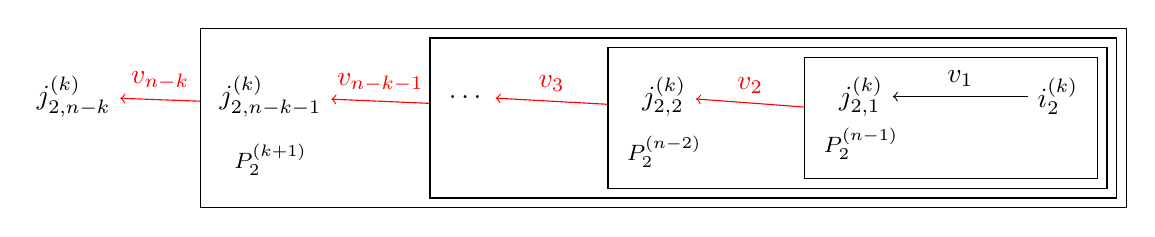
\begin{tikzpicture}
\tikzstyle{box} = [rectangle, minimum width=2cm, minimum height=1cm, text centered, draw=black]
\draw (0,0) node (A) {$j^{(k)}_{2,n-k}$} +(2.5,0) node (B) {$j^{(k)}_{2,n-k-1}$}+(2.5,-.8) node (P1) {\footnotesize$P_2^{(k+1)}$} +(5,0) node (B1) {$\dots$} +(7.5,0) node (C) {$j^{(k)}_{2,2}$} +(7.5,-.7) node (P3) {\footnotesize$P_2^{(n-2)}$}+(10,0) node (D) {$j^{(k)}_{2,1}$}  +(12.5,0) node (E) {$i^{(k)}_2$} +(10,-.6) node (P4) {\footnotesize$P_2^{(n-1)}$}; 
\node (Q1) [draw=black,fit={(D) (E) (P4)}]{};
\node (Q2) [draw=black,fit={(Q1) (C) (P3)}]{};
\node (Q2b)[draw=black,fit={(Q2) (B1) }]{};

\node (Q3)[draw=black,fit={(Q2b) (B) (P1)}]{};
\draw[<-] (D)--(E) node[pos=.5,above] {$v_1$};
\draw[->,red] (Q1)--(C) node[pos=.5,above] {$v_2$};
\draw[->,red] (Q2)--(B1) node[pos=.5,above] {$v_3$};
\draw[->,red] (Q2b)--(B) node[pos=.5,above] {$v_{n-k-1}$};

\draw[->,red] (Q3)--(A) node[pos=.5,above] {$v_{n-k}$};
\end{tikzpicture}
\\

\noindent
where the $2$-arrows are coloured red. As the number of strong successor closed subsets of this $2$-quiver coincides with the number of successor closed subsets of the coefficient quiver, for clearness reasons, we will mostly work with the coefficient quiver instead.

The next step is to define the $2$-quivers of $P^{(k)}_3$ whence the remaining $2$-quivers can be obtained recursively. First we choose the basis of $\Ext(P_2^{(1)},P_2)$ given by the linear maps
$$\{i_2^{(n-1)}\xlongrightarrow{v_n}j_{2,i}\mid i=n-1,\ldots,1\}.$$
This basis gives rise to the following $2$-quiver of $P_3^{(k)}$ where we drop the indices of the vertices in abuse of notation.
\\

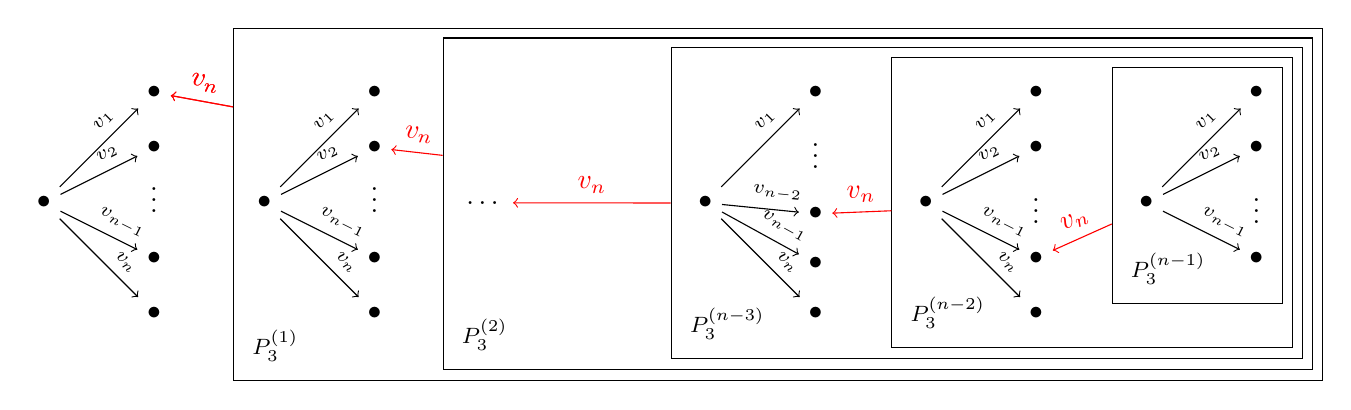
\begin{tikzpicture}[scale=1.4]
\draw (0,0) node (I1) {$\bullet$} +(1,1) node (J11) {$\bullet$} +(1,.5) node (J12) {$\bullet$} +(1,0.1) node (D1) { $\vdots$}+(1,-.5) node (J1N1) {$\bullet$} +(1,-1) node (J1N) {$\bullet$} ; 
\draw[->] (I1)--(J11) node[pos=.7,above,sloped]{\scriptsize$v_1$};
\draw[->] (I1)--(J12) node[pos=.7,above,sloped]{\scriptsize$v_2$};
\draw[->] (I1)--(J1N1) node[pos=.7,above,sloped]{\scriptsize$v_{n-1}$};
\draw[->] (I1)--(J1N) node[pos=.7,above,sloped]{\scriptsize$v_{n}$};

\draw (2,0) node (I2) {$\bullet$} +(1,1) node (J21) {$\bullet$} +(1,.5) node (J22) {$\bullet$}+(1,0.1) node (D2) { $\vdots$} +(1,-.5) node (J2N1) {$\bullet$} +(1,-1) node (J2N) {$\bullet$} +(0.1,-1.3) node (P1) {\footnotesize$P_3^{(1)}$} ; 
\draw[->] (I2)--(J21) node[pos=.7,above,sloped]{\scriptsize$v_1$};
\draw[->] (I2)--(J22) node[pos=.7,above,sloped]{\scriptsize$v_2$};
\draw[->] (I2)--(J2N1) node[pos=.7,above,sloped]{\scriptsize$v_{n-1}$};
\draw[->] (I2)--(J2N) node[pos=.7,above,sloped]{\scriptsize$v_{n}$};

\draw (4,0) node (DOTS) {$\dots$}+(0,-1.2) node (P2b) {\footnotesize$P_3^{(2)}$};

\draw (6,0) node (I3) {$\bullet$} +(1,1) node (J31) {$\bullet$}   +(1,.5) node (D31) { $\vdots$} +(1,-.1) node (J3N2) {$\bullet$} +(1,-.55) node (J3N1) { $\bullet$} +(1,-1) node (J3N) {$\bullet$} +(0.2,-1.1) node (P3) {\footnotesize$P_3^{(n-3)}$} ; 
\draw[->] (I3)--(J31) node[pos=.7,above,sloped]{\scriptsize$v_1$};
\draw[->] (I3)--(J3N2) node[pos=.7,above,sloped]{\scriptsize$v_{n-2}$};
\draw[->] (I3)--(J3N1) node[pos=.7,above,sloped]{\scriptsize$v_{n-1}$};
\draw[->] (I3)--(J3N) node[pos=.7,above,sloped]{\scriptsize$v_{n}$};

\draw (8,0) node (I4) {$\bullet$} +(1,1) node (J41) {$\bullet$} +(1,.5) node (J42) {$\bullet$} +(1,0) node (D4) { $\vdots$} +(1,-.5) node (J4N1) {$\bullet$} +(1,-1) node (J4N) {$\bullet$} +(0.2,-1) node (P4) {\footnotesize$P_3^{(n-2)}$}; 
\draw[->] (I4)--(J41) node[pos=.7,above,sloped]{\scriptsize$v_1$};
\draw[->] (I4)--(J42) node[pos=.7,above,sloped]{\scriptsize$v_2$};
\draw[->] (I4)--(J4N1) node[pos=.7,above,sloped]{\scriptsize$v_{n-1}$};
\draw[->] (I4)--(J4N) node[pos=.7,above,sloped]{\scriptsize$v_{n}$};

\draw (10,0) node (I5) {$\bullet$} +(1,1) node (J51) {$\bullet$} +(1,.5) node (J52) {$\bullet$} +(1,0) node (D5) { $\vdots$} +(1,-.5) node (J5N1) {$\bullet$} +(0.2,-.6) node (P5) {\footnotesize$P_3^{(n-1)}$}   ; 
\draw[->] (I5)--(J51) node[pos=.7,above,sloped]{\scriptsize $v_1$};
\draw[->] (I5)--(J52) node[pos=.7,above,sloped]{\scriptsize $v_2$};
\draw[->] (I5)--(J5N1) node[pos=.7,above,sloped]{\scriptsize $v_{n-1}$};
%\tikzstyle{every node}=[circle,fill=white!10]
\node (Q2) [draw=black,fit={(P5) (I5) (J51) (J52) (J5N1)}]{};
%\node (R2) [draw=black,fit={(I4) (J4N1)}, sloped]{};
\draw[->,red] (Q2)--(J4N1) node[pos=.5,above,sloped]{$v_{n}$};
\node (Q3) [draw=black,fit={(P4) (Q2) (I4) (J41) (J42) (J4N1) (J4N)}]{};
\draw[->,red] (Q3)--(J3N2)  node[pos=.5,above,sloped] {$v_{n}$};
\node (Q4) [draw=black,fit={(P3) (Q3) (I3) (J31) (J3N1) (J3N2) (J3N)}]{};
\draw[->,red] (Q4)--(DOTS)  node[pos=.5,above] {$v_{n}$};
\node (Q4b) [draw=black,fit={(P2b) (Q4) (DOTS)}]{};

\node (Q5) [draw=black,fit={(P1) (Q4b) (I2) (J21) (J22) (J2N1) (J2N)}]{};
\draw[->,red] (Q5)--(J11)  node[pos=.5,above,sloped,sloped] {$v_{n}$};
\draw[->,red] (Q4b)--(J22)  node[pos=.5,above,sloped] {$v_{n}$};
\draw[->,red] (Q5)--(J11)  node[pos=.5,above,sloped] {$v_{n}$};

\end{tikzpicture}
\\

We have $\dim \Hom(P_m,\tau P_m^{(k)})=\dim\Ext(P_m^{(k)},P_m)=n-k$. If a basis of $\Ext(P_m^{(k)},P_m)$ is compatible with a lift to the universal covering, Lemma \ref{AR} gives a one-to-one correspondence between basis elements of $\Ext(P_m^{(k)},P_m)$ and $\Hom(P_{m-1},\tau P_m^{(k)})$. Let us consider the case $m=3$. The coefficient quiver of $\tau P_3^{(k)}$ is given by
\[\xymatrix@R10pt@C20pt{&&i_{1}\ar_{v_1}[lld]\\ j &&\vdots\\&&i_{k}\ar_{v_{k}}[llu]}.\]
The image of the homomorphism of the corresponding exact sequence induced by the basis element $i_2^{(n-1)}\xrightarrow{v_n} j_{2,l}$ is the quotient quiver $j\xlongleftarrow{v_l} i_l$. Thus in this case the $2$-arrow connects the $2$-quiver of $P_3^{(k)}$ to the image of the corresponding homomorphism $P_2\to P_1^{(k)}$ which is of dimension $(1,1)$. In the above illustration, we forgo to insert the corresponding rectangles and just connected the $2$-arrows to the sinks of the corresponding subquivers. It can be seen that this is no restriction from the combinatorial point of view. 

Now we can recursively the $2$-quivers of $P_m^{(k)}$ for $m\geq 4$ and $k=n-1,\ldots,0$ when repeating this procedure. For $m\geq 4$, the truncated preprojective $\tau P_m^{(k)}$ can uniquely be found as a quotient of $P_m$.
Recall that we have $\udim P_m^{(k)}=\udim P_{m-1}^{(1)}+(n-k-1)\udim P_{m-1}$. Moreover, we have 
\[\dim \Hom(P_{m-1},\tau P_m^{(1)})=\dim\Ext(P_m^{(1)},P_{m-1})=n-1.\]

As before we get a one-to-one correspondence between basis elements when passing to the universal covering quiver. More precisely, we can take the BGP-reflected basis of the basis of $\Ext(P_2^{(1)},P_2)$ from above.

Let us assume that we already constructed the $2$-quiver of $P_{m+1}^{(k)}$. The $2$-quiver of $P^{(k-1)}_{m+1}$ is given by glueing the $2$-quiver of $P_{m+1}^{(k)}$ to the one of $P_{m}$
\\

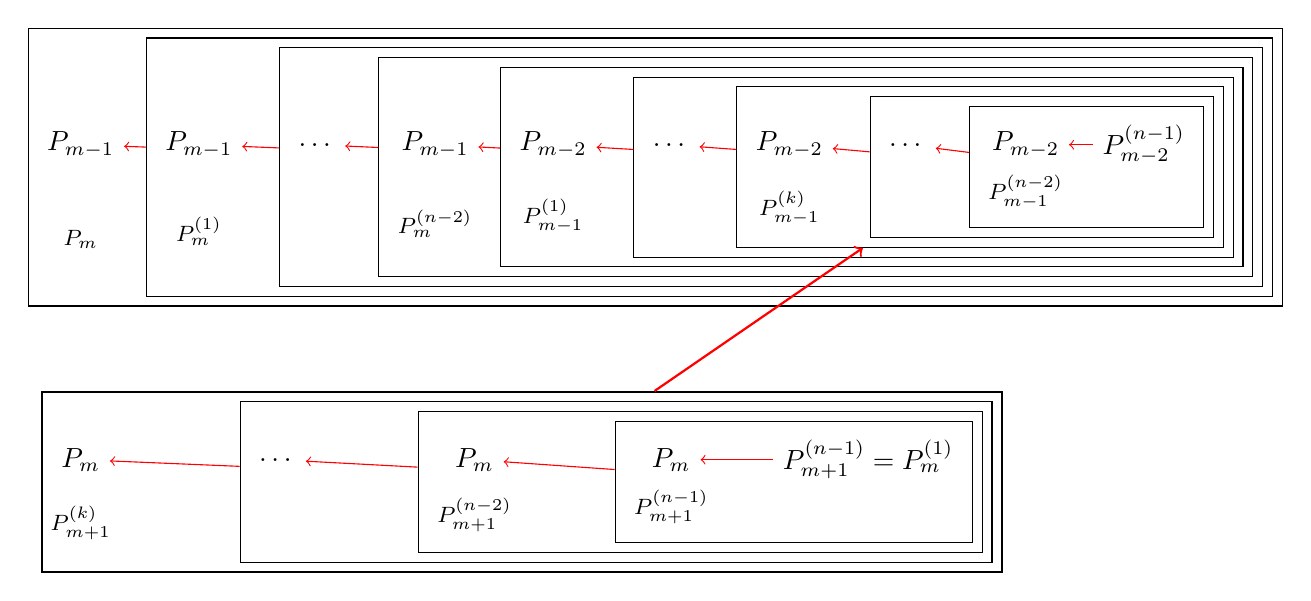
\begin{tikzpicture}
\draw (0,4) node (A1) {$P_{m-1}$}+(0,-1.2) node (PM) {\footnotesize$P_{m}$} +(1.5,0) node (B1) {$P_{m-1}$}+(1.5,-1.1) node (P11) {\footnotesize$P_{m}^{(1)}$} +(3,0) node (B11) {$\dots$} +(4.5,0) node (D1) {$P_{m-1}$}  +(6,0) node (E1) {$P_{m-2}$} +(4.5,-1) node (P41) {\footnotesize$P_{m}^{(n-2)}$}+(6,-.9) node (P51) {\footnotesize$P_{m-1}^{(1)}$}+(7.5,0) node (A1b) {$\dots$} +(9,0) node (B1b) {$P_{m-2}$}+(9,-.8) node (P11b) {\footnotesize$P_{m-1}^{(k)}$} +(10.5,0) node (B11b) {$\dots$} +(12,0) node (D1b) {$P_{m-2}$} +(12,-.6) node (P41b) {\footnotesize$P_{m-1}^{(n-2)}$} +(13.5,0) node (E1b) {$P^{(n-1)}_{m-2}$} ; 
\node (Q11) [draw=black,fit={(D1b) (E1b) (P41b)}]{};
\node (Q21) [draw=black,fit={(Q11) (B11b)}]{};
\node (Q31)[draw=black,fit={(Q21) (B1b) (P11b)}]{};
\node (Q41)[draw=black,fit={(Q31) (A1b)}]{};
\node (Q51)[draw=black,fit={(Q41) (E1)}]{};
\node (Q61)[draw=black,fit={(Q51) (P41) (D1)}]{};
\node (Q71)[draw=black,fit={(Q61) (B11)}]{};
\node (Q81)[draw=black,fit={(Q71) (P11) (B1)}]{};
\node (Q91)[draw=black,fit={(Q81) (A1)}]{};
\draw[<-,red] (D1b)--(E1b) node[pos=.5,above] {};
\draw[->,red] (Q11)--(B11b) node[pos=.5,above] {};
\draw[->,red] (Q21)--(B1b) node[pos=.5,above] {};
\draw[->,red] (Q31)--(A1b) node[pos=.5,above] {};
\draw[->,red] (Q41)--(E1) node[pos=.5,above] {};
\draw[->,red] (Q51)--(D1) node[pos=.5,above] {};
\draw[->,red] (Q61)--(B11) node[pos=.5,above] {};
\draw[->,red] (Q71)--(B1) node[pos=.5,above] {};
\draw[->,red] (Q81)--(A1) node[pos=.5,above] {};

\draw (0,0) node (B) {$P_{m}$}+(0,-.8) node (P1) {\footnotesize$P_{m+1}^{(k)}$} +(2.5,0) node (B1) {$\dots$} +(5,0) node (C) {$P_{m}$} +(5,-.7) node (P3) {\footnotesize$P_{m+1}^{(n-2)}$}+(7.5,0) node (D) {$P_{m}$}  +(10,0) node (E) {$P_{m+1}^{(n-1)}=P_{m}^{(1)}$} +(7.5,-.6) node (P4) {\footnotesize$P_{m+1}^{(n-1)}$}; 
\node (Q1) [draw=black,fit={(D) (E) (P4)}]{};
\node (Q2) [draw=black,fit={(Q1) (C) (P3)}]{};
\node (Q2b)[draw=black,fit={(Q2) (B1) }]{};

\draw[<-,red] (D)--(E) node[pos=.5,above] {};
\draw[->,red] (Q1)--(C) node[pos=.5,above] {};
\draw[->,red] (Q2)--(B1) node[pos=.5,above] {};
\draw[->,red] (Q2b)--(B) node[pos=.5,above] {};

\node (PMK) [draw=black, thick,fit={(Q2b) (B)}]{};
\draw[->,red,thick] (PMK)--(Q31);
\end{tikzpicture}
\\

\noindent where the $2$-arrows connects the $2$-quiver of $P_{m+1}^{(k)}$ to its Auslander-Reiten translate $\tau P_{m+1}^{(k)}= P_{m-1}^{(k)}$ in $P_m$. This subquiver can be found at the very right of the $2$-quiver of $P_m$. Note that forgo the colouring of the arrows as it does not play any role from the combinatorial point of view. For $n=3$ the $2$-quiver of $P_3$ is given by:\\

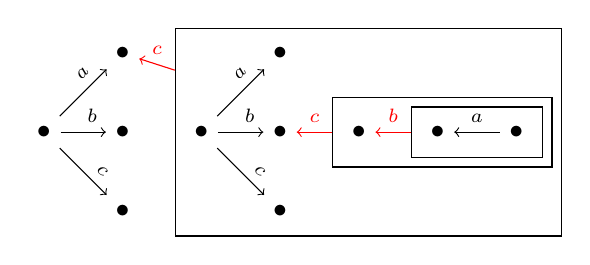
\begin{tikzpicture}[scale=1]
\draw (0,0) node (I1) {$\bullet$} +(1,1) node (J11) {$\bullet$} +(1,0) node (J12) {$\bullet$} +(1,-1) node (J13) {$\bullet$}; 
\draw[->] (I1)--(J11) node[pos=.7,above,sloped]{\scriptsize$a$};
\draw[->] (I1)--(J12) node[pos=.7,above,sloped]{\scriptsize$b$};
\draw[->] (I1)--(J13) node[pos=.7,above,sloped]{\scriptsize$c$};
%\draw[->] (I1)--(J1N) node[pos=.7,above,sloped]{\scriptsize$v_{n}$};

\draw (2,0) node (I2) {$\bullet$} +(1,1) node (J21) {$\bullet$} +(1,0) node (J22) {$\bullet$} +(1,-1) node (J23) {$\bullet$}; 
\draw[->] (I2)--(J21) node[pos=.7,above,sloped]{\scriptsize$a$};
\draw[->] (I2)--(J22) node[pos=.7,above,sloped]{\scriptsize$b$};
\draw[->] (I2)--(J23) node[pos=.7,above,sloped]{\scriptsize$c$};
%\draw[->] (I1)--(J1N) node[pos=.7,above,sloped]{\scriptsize$v_{n}$};
\draw (6,0) node (I3) {$\bullet$} (5,0) node (J31) {$\bullet$} (4,0) node (J33) {$\bullet$}; 
\draw[->] (I3)--(J31) node[pos=.5,above,sloped]{\scriptsize$a$};
%\draw[->] (I3)--(J32) node[pos=.7,above,sloped]{\scriptsize$b$};
%\draw[->] (I3)--(J33) node[pos=.7,above,sloped]{\scriptsize$c$};
%\draw[->] (I1)--(J1N) node[pos=.7,above,sloped]{\scriptsize$v_{n}$};
\node (Q0)[draw=black,fit={(I3) (J31) }]{};
\node (Q1)[draw=black,fit={(Q0) (J33)}]{};
\node (Q2)[draw=black,fit={(Q1) (I2) (J21) (J22) (J23)}]{};

%\node (Q3)[draw=black,fit={(Q2b) (B) (P1)}]{};
\draw[->,red] (Q0)--(J33) node[pos=.5,above] {\scriptsize $b$};
\draw[->,red] (Q1)--(J22) node[pos=.5,above] {\scriptsize $c$};
\draw[->,red] (Q2)--(J11) node[pos=.5,above] {\scriptsize $c$};
\end{tikzpicture}
\\

The one of $P_4$ is given by:\\

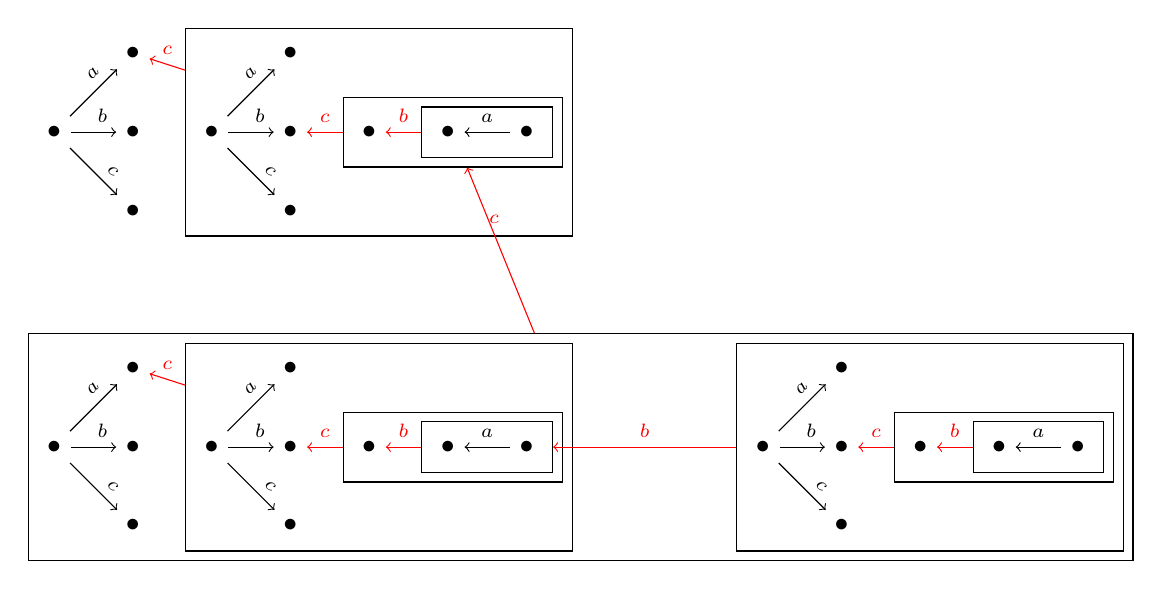
\begin{tikzpicture}[scale=1]
\draw (0,0) node (I1) {$\bullet$} +(1,1) node (J11) {$\bullet$} +(1,0) node (J12) {$\bullet$} +(1,-1) node (J13) {$\bullet$}; 
\draw[->] (I1)--(J11) node[pos=.7,above,sloped]{\scriptsize$a$};
\draw[->] (I1)--(J12) node[pos=.7,above,sloped]{\scriptsize$b$};
\draw[->] (I1)--(J13) node[pos=.7,above,sloped]{\scriptsize$c$};
%\draw[->] (I1)--(J1N) node[pos=.7,above,sloped]{\scriptsize$v_{n}$};

\draw (2,0) node (I2) {$\bullet$} +(1,1) node (J21) {$\bullet$} +(1,0) node (J22) {$\bullet$} +(1,-1) node (J23) {$\bullet$}; 
\draw[->] (I2)--(J21) node[pos=.7,above,sloped]{\scriptsize$a$};
\draw[->] (I2)--(J22) node[pos=.7,above,sloped]{\scriptsize$b$};
\draw[->] (I2)--(J23) node[pos=.7,above,sloped]{\scriptsize$c$};
%\draw[->] (I1)--(J1N) node[pos=.7,above,sloped]{\scriptsize$v_{n}$};
\draw (6,0) node (I3) {$\bullet$} (5,0) node (J31) {$\bullet$} (4,0) node (J33) {$\bullet$}; 
\draw[->] (I3)--(J31) node[pos=.5,above,sloped]{\scriptsize$a$};
%\draw[->] (I3)--(J32) node[pos=.7,above,sloped]{\scriptsize$b$};
%\draw[->] (I3)--(J33) node[pos=.7,above,sloped]{\scriptsize$c$};
%\draw[->] (I1)--(J1N) node[pos=.7,above,sloped]{\scriptsize$v_{n}$};
\node (Q0)[draw=black,fit={(I3) (J31) }]{};
\node (Q1)[draw=black,fit={(Q0) (J33)}]{};
\node (Q2)[draw=black,fit={(Q1) (I2) (J21) (J22) (J23)}]{};

%\node (Q3)[draw=black,fit={(Q2b) (B) (P1)}]{};
\draw[->,red] (Q0)--(J33) node[pos=.5,above] {\scriptsize $b$};
\draw[->,red] (Q1)--(J22) node[pos=.5,above] {\scriptsize $c$};
\draw[->,red] (Q2)--(J11) node[pos=.5,above] {\scriptsize $c$};


\draw (0,-4) node (I1b) {$\bullet$} +(1,1) node (J11b) {$\bullet$} +(1,0) node (J12b) {$\bullet$} +(1,-1) node (J13b) {$\bullet$}; 
\draw[->] (I1b)--(J11b) node[pos=.7,above,sloped]{\scriptsize$a$};
\draw[->] (I1b)--(J12b) node[pos=.7,above,sloped]{\scriptsize$b$};
\draw[->] (I1b)--(J13b) node[pos=.7,above,sloped]{\scriptsize$c$};
%\draw[->] (I1)--(J1N) node[pos=.7,above,sloped]{\scriptsize$v_{n}$};

\draw (2,-4) node (I2b) {$\bullet$} +(1,1) node (J21b) {$\bullet$} +(1,0) node (J22b) {$\bullet$} +(1,-1) node (J23b) {$\bullet$}; 
\draw[->] (I2b)--(J21b) node[pos=.7,above,sloped]{\scriptsize$a$};
\draw[->] (I2b)--(J22b) node[pos=.7,above,sloped]{\scriptsize$b$};
\draw[->] (I2b)--(J23b) node[pos=.7,above,sloped]{\scriptsize$c$};

\draw (6,-4) node (I3b) {$\bullet$} (5,-4) node (J31b) {$\bullet$} (4,-4) node (J33b) {$\bullet$}; 
\draw[->] (I3b)--(J31b) node[pos=.5,above,sloped]{\scriptsize$a$};
\node (Q0b)[draw=black,fit={(I3b) (J31b) }]{};
\node (Q1b)[draw=black,fit={(Q0b) (J33b)}]{};
\node (Q2b)[draw=black,fit={(Q1b) (I2b) (J21b) (J22b) (J23b)}]{};

\draw[->,red] (Q0b)--(J33b) node[pos=.5,above] {\scriptsize $b$};
\draw[->,red] (Q1b)--(J22b) node[pos=.5,above] {\scriptsize $c$};
\draw[->,red] (Q2b)--(J11b) node[pos=.5,above] {\scriptsize $c$};

\draw (9,-4) node (I2c) {$\bullet$} +(1,1) node (J21c) {$\bullet$} +(1,0) node (J22c) {$\bullet$} +(1,-1) node (J23c) {$\bullet$}; 
\draw[->] (I2c)--(J21c) node[pos=.7,above,sloped]{\scriptsize$a$};
\draw[->] (I2c)--(J22c) node[pos=.7,above,sloped]{\scriptsize$b$};
\draw[->] (I2c)--(J23c) node[pos=.7,above,sloped]{\scriptsize$c$};

\draw (13,-4) node (I3c) {$\bullet$} (12,-4) node (J31c) {$\bullet$} (11,-4) node (J33c) {$\bullet$}; 
\draw[->] (I3c)--(J31c) node[pos=.5,above,sloped]{\scriptsize$a$};
\node (Q0c)[draw=black,fit={(I3c) (J31c) }]{};
\node (Q1c)[draw=black,fit={(Q0c) (J33c)}]{};
\node (Q2c)[draw=black,fit={(Q1c) (I2c) (J21c) (J22c) (J23c)}]{};
\node (Q3c)[draw=black,fit={(Q2c) (Q2b) (I1b)}]{};
\draw[->,red] (Q0c)--(J33c) node[pos=.5,above] {\scriptsize $b$};
\draw[->,red] (Q1c)--(J22c) node[pos=.5,above] {\scriptsize $c$};
\draw[->,red] (Q2c)--(Q0b) node[pos=.5,above] {\scriptsize $b$};
\draw[->,red] (Q3c)--(Q1) node[pos=.6,above] {\scriptsize $c$};

\end{tikzpicture}



\begin{theorem}
  The Euler characteristic $\chi(\Gr_e(P_m^{(k)}))$ is given by the number of strong successor closed subsets of type $e$ of the $2$-quiver of $P_m^{(k)}$.
\end{theorem}
\begin{proof}
  We proceed by induction.
  The strong successor closed subsets of the $2$-quivers of $P_1$, $P_2$ and $P_2^{(n-1)}$ coincide with the successor closed subsets of the coefficient quivers (\ref{coeff}) which we denote by $\Gamma_M$ for $M\in\{P_1, P_2,P_2^{(n-1)}\}$.
  Passing to the universal cover, we have $\Gr_e(\tilde M)\in\{\emptyset,\{\pt\}\}$ such that $\Gr_e(\tilde M)=\{\pt\}$ if and only if $e\subset (\Gamma_M)_0$ is successor closed.
  As the number cells of $\Gr_e(\tilde M)$ and $\Gr_e(M)$ coincide, the claim follows.

  Thus assume that the claim is true for $P_m$ (resp. $\tilde P_{m}$) and $P_{m+1}^{(k)}$ (resp. $\tilde P_{m+1}^{(k)}$) and consider the short exact sequence
  \[
    \ses{\tilde P_m}{\tilde P_{m+1}^{(k-1)}}{\tilde P_{m+1}^{(k)}}.
  \]
  Denote the corresponding $2$-quivers by $\Gamma_{P_m}$ and $\Gamma_{P_{m+1}^{(k)}}$ and let $\beta_1\cup\beta_2\subset (\Gamma_{P_m})_0\cup (\Gamma_{P_{m+1}^{(k)}})_0$ be a pair of strong successor closed subsets which gives rise to a pair of non-empty cell by induction hypothesis.
  Denote by $d(\beta_1+\beta_2)$ the dimension vector corresponding to this subset.
  By Proposition \ref{fibers} the pair $\beta_1\cup\beta_2$, it does not correspond to a non-empty cell of $\Gr_{d(\beta_1+\beta_2)}(\tilde P_{m+1}^{(k)})$ if and only if $\beta_2=(\Gamma_{P_{m+1}^{(k)}})_0$ and $\beta_1\cap(\Gamma_{\tau\tilde P_{m+1}^{(k)}})_0=\emptyset$.
  But this is precisely the condition on $\beta_1\cup\beta_2$ to be strong successor closed as $\Gamma_{P_{m+1}^{(k)}}$ is connected to $\Gamma_{\tau\tilde P_{m+1}^{(k)}}$ by a $2$-arrow.
\end{proof}


%%%%%%%%%%%%%%%%%%%%%%%%%%%%%%%%%%%%%%%%%%%%%%%%%%%%%%%%%%
\subsection{Compatible Pairs}
For $m\ge1$, let $D_m$ denote the maximal Dyck path in the lattice rectangle with corner vertices $(0,0)$ and $(u_m,u_{m-1})$.  
More precisely, $D_m$ is the lattice path which begins at $(0,0)$, takes East and North steps to end at $(u_m,u_{m-1})$, and never passes above the main diagonal joining $(0,0)$ and $(u_m,u_{m-1})$.  
It is maximal in the sense that any lattice point lying strictly above $D_m$ also lies above the main diagonal.  

The maximal Dyck paths $D_m$, $m\ge1$, exhibit the following recursive structure.
In what follows we assume $n\ge2$.
\begin{theorem}
  \cite[Corollary 2.4]{rupel}
  \label{th:dyck path recursion}
  For $n\ge2$, the maximal Dyck path $D_m$, $m\ge1$, can be constructed recursively as follows:
  \begin{enumerate}
    \item $D_1$ consists of a single horizontal edge;
    \item $D_2$ consists of $n$ consecutive horizontal edges followed by a vertical edge;
    \item $D_m$, $m\ge3$, consists of $n-1$ copies of $D_{m-1}$ followed by a copy of $D_{m-1}$ with its first $D_{m-2}$ removed.
  \end{enumerate}
\end{theorem}

We obtain the following as an immediate consequence.
\begin{corollary}
  \label{cor:short hooks}
  Inside $D_m$, $m\ge2$, there are precisely $u_{m-2}$ vertical edges which are immediately preceded by exactly $n-1$ horizontal edges.
\end{corollary}
\begin{proof}
  We work by induction on $m\ge2$.
  The cases $m=2,3$ are immediate from Theorem~\ref{th:dyck path recursion} parts (2) and (3).
  For $m\ge4$, part (3) of Theorem~\ref{th:dyck path recursion} shows by induction that there are $(n-1)u_{m-3}+(u_{m-3}-u_{m-4})=u_{m-2}$ vertical edges which are immediately preceded by exactly $n-1$ horizontal edges.
\end{proof}

For $m\ge2$ and $1\le k\le n-1$, write $D_m^{(k)}$ for the maximal Dyck path obtained from $D_m$ by removing the first $k$ copies of $D_{m-1}$.
Extending this notation we also set $D_m^{(0)}:=D_m$.
\begin{remark}
  Note that by Theorem~\ref{th:dyck path recursion}, we have a natural identification of $D_m^{(n-1)}$, $m\ge3$, with $D_{m-1}^{(1)}$.
\end{remark}
For fixed $m\ge2$ and $1\le r\le n-1$, we write $D_{m-1,r}$ for the $r$-th copy of $D_{m-1}$ inside $D_m$.
For notational convenience we also set $D_{m-1,n}:=D_m^{(n-1)}$ even though this maximal Dyck path does not identify with a copy of $D_{m-1}$.
For $m\ge2$ and $1\le k\le n-1$, the maximal Dyck paths $D_{m-1,r}$, $k+1\le r\le n$, naturally identify with subpaths of $D_m^{(k)}$.

We identify the edges of $D_m$ with the ordered set $E_m=\{1,\ldots,u_m+u_{m-1}\}$, where edges of $D_m$ are taken in the natural order beginning from $(0,0)$.
Let $E_m=H_m\sqcup V_m$, where $H_m=\{h_1,\ldots,h_{u_m}\}$ and $V_m=\{v_1,\ldots,v_{u_{m-1}}\}$ denote the horizontal and vertical edges of $D_m$ respectively.
Following Theorem~\ref{th:dyck path recursion}, we partition the edges as $E_m=\bigsqcup_{r=1}^n E_{m-1,r}$, where $E_{m-1,r}$ denotes the edges of $D_{m-1,r}$.
The set $E_{m-1,r}$ is naturally partitioned into its subsets $H_{m-1,r}$ and $V_{m-1,r}$ of horizontal and vertical edges.

Given edges $e,e'\in E_m$ with $e<e'$, write $ee'$ for the shortest subpath of $D_m$ containing $e$ and $e'$, in particular $ee$ is the subpath containing the single edge $e$.
\begin{definition}
  \label{def:compatibility}
  A pair of subsets $S_H\subset H_m$ and $S_V\subset V_m$ is called \emph{compatible} if: 
  for each pair $(h,v)\in S_H\times S_V$ with $h<v$ there exists an edge $e\in hv$ so that at least one of the following holds
  \begin{equation}
    \label{eq:hgc}
    e\ne v\qquad\text{and}\qquad |he\cap V_m|=n|he\cap S_H|
  \end{equation}
  or
  \begin{equation}
    \label{eq:vgc}
    e\ne h\qquad\text{and}\qquad |ev\cap H_m|=n|ev\cap S_V|.
  \end{equation}
  Write $\cC_m$ for the collection of all pairs $(S_H,S_V)$ which are compatible as above.
\end{definition}
\begin{remark}
  This notion of compatibility extends naturally to the maximal Dyck paths $D_m^{(k)}$, $1\le k\le n-1$.  Write $\cC_m^{(k)}$ for the set of all compatible pairs in $D_m^{(k)}$.
\end{remark}

The recursive structure of the maximal Dyck paths from Theorem~\ref{th:dyck path recursion} gives rise to a recursive characterization of compatible pairs.
\begin{definition}
  \cite[Definition 3.11]{rupel}
  \label{def:piecewise compatibility}
  A pair of subsets $S_H\subset H_m$ and $S_V\subset V_m$ is called \emph{piecewise compatible} if, for each $1\le r\le n$, one of the conditions \eqref{eq:hgc} or \eqref{eq:vgc} is satisfied for each pair $(h,v)\in S_H\times S_V$ with $h\in H_{m-1,r}$ and $v\in V_{m-1,r}$.
\end{definition}
\begin{remark}
  The notion of piecewise compatibility naturally extends to the maximal Dyck paths $D_m^{(k)}$, $1\le k\le n-1$.
\end{remark}

To describe precisely when a piecewise compatible pair $(S_H,S_V)$ is compatible we need more notation.
For a horizontal edge $h\in H_m$ and a subset $S_H\subset H_m$, write $D(h;S_H)=he$ for the shortest subpath of $D_m$ for which $|he\cap V_m|=n|he\cap S_H|$, if no such subpath exists we set $D(h;S_H)=hv_{u_{m-1}}$.
The subpath $D(h;S_H)$ is called the \emph{local shadow path} of $h$ with respect to $S_H$.
Similarly, for a vertical edge $v\in V_m$ and a subset $S_V\subset V_m$, the \emph{local shadow path} of $v$ with repect to $S_V$ is $D(v;S_V)=ev$ for the shortest subpath of $D_m$ for which $|ev\cap H_m|=n|ev\cap S_V|$ and we take $D(v;S_V)=h_1v$ if there does not exist such an edge $e$.
\begin{definition}
  \cite[Definition 3.17]{rupel}
  A horizontal edge $h_i\in H_m$, $m\ge3$, is called \emph{blocking} for a subset $S_H\subset H_m$ if $D(h_i;S_H)=h_iv_{u_{m-1}}$ and $h_i$ is furthest to the right with this property, i.e.\ the index $i$ is maximal with this property. 

  Suppose $S_H\subset H_m$ admits a blocking edge $h_i\in H_m$.
  Then $S_H$ is \emph{left-justified at $h_i$} if there exists $k\ge i$ so that $S_H=\{h_i,h_{i+1},\ldots,h_k\}$.
  The subset $S_H$ is \emph{strongly left-justified at $h_i$} if $S_H$ is left-justified at $h_i$ and $|h_iv_{u_{m-1}}\cap V_m|=n|h_iv_{u_{m-1}}\cap S_H|$.

  A subset $S_V\subset V_m$ is \emph{right-justified with respect to $h_i$} if there exists a vertical edge $v_s\in h_iv_{u_{m-1}}$ so that $S_V\cap h_iv_{u_{m-1}}=\{v_s,v_{s-1},\ldots,v_{u_{m-1}}\}$.
  The subset $S_V$ is \emph{strongly right-justified with respect to $h_i$} if $S_V$ is right-justified with respect to $h_i$ and $D(v_{u_{m-1}};S_V)=h_iv_{u_{m-1}}$ with $|h_iv_{u_{m-1}}\cap H_m|=n|h_iv_{u_{m-1}}\cap S_V|$.
\end{definition}

\begin{theorem}
  \cite[Theorem 3.20 and Corollary 3.22]{rupel}
  \label{th:blocking edge conditions}
  For $m\ge3$, suppose $S_H\subset H_m$ and $S_V\subset V_m$ are piecewise compatible. 
  Then the following hold:
  \begin{enumerate}
    \item If $S_H$ does not admit a blocking edge, then $(S_H,S_V)\in\cC_m$.
    \item Suppose $S_H$ admits a blocking edge $h_i\in H_m$ and $(S_H,S_V)$ is not compatible.
      Then $S_H$ is left-justified at $h_i$ and $S_V$ is strongly right-justified with respect to $h_i$.
      In addition the following hold:
      \begin{enumerate}
        \item If $m=3$, then $S_H\cap h_iv_{u_{m-1}}=\{h_i\}$.
        \item If $m\ge4$, then $S_H$ is strongly left-justified at $h_i$.
        \item If $m\ge5$, then either $i=1$ or $h_i$ is immediately preceded by a vertical edge in $D_m$.
      \end{enumerate}
  \end{enumerate}
\end{theorem}

\begin{corollary}
  For $m\ge4$ and $0\le k\le n-1$, consider $S_H\subset H_m^{(k)}$ and $S_V\subset V_m^{(k)}$ so that $(S_H,S_V)$ is piecewise compatible.
  Assume $\big(S_H^{(k+1)},S_V^{(k+1)}\big)\in\cC_m^{(k+1)}$.
  Then $(S_H,S_V)$ is not compatible if and only if $H_{m-2}^{(k+1)}\subset S_{H,k+1}$ and $V_m^{(k+1)}\subset S_V$.
\end{corollary}
\begin{proof}
  We begin with the reverse implication.
  First note that there are $(n-k)u_{m-1}-u_{m-2}$ horizontal edges and $(n-k)u_{m-2}-u_{m-3}$ vertical edges in $D_m^{(k)}$. 
  It follows that $V_{m-2}^{(k+1)}\sqcup V_m^{(k+1)}$ contains $n(n-k)u_{m-3}-nu_{m-4}$ vertical edges and $H_{m-2}^{(k+1)}\sqcup H_m^{(k+1)}$ contains $n(n-k)u_{m-2}-nu_{m-3}$ horizontal edges.

  Assuming $H_{m-2}^{(k+1)}\subset S_{H,k+1}$ and $S_V^{(k+1)}=V_m^{(k+1)}$, we have $S_V\cap V_{m-2}^{(k+1)}=\varnothing$ and $S_H\cap H_m^{(k+1)}=\varnothing$ by piecewise compatibility.
  Let $h\in H_m^{(k)}$ be the horizontal edge corresponding to the first horizontal edge of $H_{m-2}^{(k+1)}$.
  Then, since there are $(n-k)u_{m-3}-u_{m-4}$ horizontal edges in $H_{m-2}^{(k+1)}$, the local shadow path $D(h;S_H)$ contains $n\big((n-k)u_{m-3}-u_{m-4}\big)$ vertical edges and is thus equal to $hv_{u_{m-1}}$.
  Similarly, the local shadow path $D(v_{u_{m-1}};S_V)$ is also equal to $hv_{u_{m-1}}$.
  In particular, neither of the compatibility conditions of Definition~\ref{def:compatibility} are satisfied for the path $hv_{u_{m-1}}$ and so $(S_H,S_V)$ is not compatible.

  For the forward implication, we work by induction on $m\ge4$.
  Consider a pair $(S_H,S_V)$ for $D_4^{(k)}$ as above which is not compatible.
  Following Theorem~\ref{th:blocking edge conditions}, write $h\in H_4^{(k)}$ for the blocking edge of $S_H$.
  Then the number of vertical edges in the local shadow path $D(h;S_H)=hv_{u_3}$ must be divisible by $n$. 
  Since $(S_H^{(k+1)},S_V^{(k+1)})$ is compatible, we must have $h\in H_{3,k}$.
  But observe that $|V_m^{(k)}|=(n-k)n-1$ and so the divisibility condition above implies $h\in H_{3,k}^{(n-1)}$.
  But $S_V$ is strongly right-justified with respect to $h$ and thus the number of horizontal edges in $D(v_{u_3};S_V)=hv_{u_3}$ is divisible by $n$.
  Identifying $H_{3,k}^{(n-1)}$ with $H_2^{(1)}$, this divisibility condition only occurs when $h$ is the first horizontal edge in $H_2^{(k+1)}\subset H_2^{(1)}$.
  Then by piecewise compatibility, the vertical edge of $H_2^{(1)}$ cannot be an element of $S_V$ and we must have $V_4^{(k+1)}\subset S_V$.
  By piecewise compatibility again, this implies $H_4^{(k+1)}\cap S_H=\varnothing$ and so $D(h;S_H)=hv_{u_3}$ implies $H_2^{(k+1)}\subset S_H$.

  To continue, let $(S_H,S_V)$ be a pair for $D_m$, $m\ge5$, which is not compatible.
  Write $\varphi:H_{m-1}\to V_m$ for the bijection given by $\varphi(h_i)=v_i$ for $1\le i\le u_{m-1}$.
  For any subset $T\subset H_{m-1}$, set $\varphi^*(T)=V_m\setminus\varphi(T)$.
  Clearly, the map $\varphi^*$ gives a bijection between subsets of $H_{m-1}$ and subsets of $V_m$.
  In Section 3.2 of \cite{rupel}, a new pair of subsets $\big((\varphi^*)^{-1}S_V,\Omega^{-1}S_H\big)$ for $D_{m-1}$ is given, we refer the reder to \emph{loc. cit} for notation.
  By \cite[Proposition 3.10]{rupel}, the pair $\big((\varphi^*)^{-1}S_V,\Omega^{-1}S_H\big)$ is not compatible, but is piecewise compatible by \cite[proposition 3.16]{rupel}.
  Thus by induction, we must have $H_{m-3}^{(k+1)}\subset(\varphi^*)^{-1}S_V$ and $V_{m-1}^{(k+1)}\subset\Omega^{-1}S_H$.
  It follows from piecewise compatibility that $H_{m-1}^{(k+1)}\cap(\varphi^*)^{-1}S_V=\varnothing$.
  But then by the definition of $\varphi^*$ we have $V_{m-2}^{(k+1)}\cap S_V=\varnothing$ and $S_V^{(k+1)}=V_m^{(k+1)}$ so that $D(v_{u_{m-1}};S_V)=hv_{u_{m-1}}$ with $h$ as in the first case above.
  Since $(S_H,S_V)$ is not compatible, Theorem~\ref{th:blocking edge conditions} states that $h$ must be the blocking edge for $S_H$ and we must have $D(h;S_H)=hv_{u_{m-1}}$.
  But this can only occur if $H_{m-2}^{(k+1)}\subset S_H$ since $H_m^{(k+1)}\cap S_H=\varnothing$ by piecewise compatibility.
\end{proof}


The following result is an immediate consequence of the combinatorial construction of rank 2 cluster variables \cite{lee-li-zelevinsky} and the categorification of these variables using representations of $K(n)$ \cite{cc,caldero-keller}.
\begin{theorem}\cite{lee-li-zelevinsky}
  For each $m\ge1$ and $\bfe\in\ZZ_{\ge0}^2$, we have $\chi\big(\Gr_\bfe(P_m)\big)=\big|\{(S_H,S_V)\in\cC_m:|S_H|=u_m-e_1,|S_V|=e_2\}\big|$.
\end{theorem}

Our goal is to show that the compatible pairs provide a natural labeling for the cells of $\chi\big(\Gr^Q_\bfe(P_m)\big)$ found in Theorem~\ref{???}.


%%%%%%%%%%%%%%%%%%%%%%%%%%%
\begin{thebibliography}{10}
\bibitem{ass}
Assem, I., Simson, D., Skowronski, A.: Elements of the Representation Theory of Associative Algebras. Cambridge University Press, Cambridge 2007.
\bibitem{ars} Auslander, M., Reiten, I., Smalo S.O.: Representation theory of Artin algebras {\bf 36}. Cambridge University Press, Cambridge 1997.
\bibitem{bb} Bialynicki-Birula, A.: Some theorems on actions of algebraic groups. Annals of Mathematics \textbf{98}, 480-497 (1973).
\bibitem{bgp}
Bernstein, I.~N., Gelfand, I.~M., Ponomarev, V.~A.: Coxeter functors, and Gabriel's theorem. Russian Mathematical Surveys \textbf{28}(2), 17-32 (1973).
\bibitem{brenner-butler} S. Benner, M.~C.~R. Butler, The equivalence of certain functors occuring in the representation theory of artin algebras and species, J. London Math. Soc., 14 (1976), 183-187.
\bibitem{cc} P., Chapoton, F.: Cluster algebras as {H}all algebras of quiver representations.
Commentarii Mathematici Helvetici \textbf{81}(3), 595-616 (2006).
\bibitem{ck}
  P. Caldero, B. Keller: From triangulated categories to cluster algebras II.  Ann. Sci. \'Ecole Norm. Sup. (4) \textbf{39} (2006), no. 6, pp.~983--1009.
\bibitem{cefr} Cerulli Irelli, Esposito, Franzen, Reineke: Topology of Quiver Grassmannians. Preprint 2017.
\bibitem{cr}
Caldero, P., Reineke, M.: On the quiver Grassmannian in the acyclic case.
Journal of Pure and Applied Algebra \textbf{212}(11), 2369-2380 (2008).
\bibitem{cj} Crawley-Boevey, W., Jensen, Bernt Tore: A note on sub-bundles of vector bundles. Glasgow Mathematical Journal \textbf{48}, 459-462 (2006).

\bibitem{gab} Gabriel, P.: The universal cover of a finite-dimensional algebra. Representations of algebras. Lecture Notes in Mathematics {\bf 903}, 68-105 (1981).
\bibitem{hr} Happel, D., Ringel, C.M.: Tilted Algebras. Transactions of the American Mathematical Society {\bf 274}, no.2, 399-443 (1982).
\bibitem{llz} K. Lee, L. Li, A. Zelevinsky: Greedy elements in rank 2 cluster algebras. Selecta Math. \textbf{20} (2014) pp.~57--82.
\bibitem{rin1} Claus Michael Ringel. Exceptional modules are tree modules. \textit{Linear algebra and its Applications}, 275/276:471-493, 1998.
\bibitem{rin} Ringel, C.M.: Reflection functors for hereditary algebras. Journal of the London Mathematical Society (2) {\bf 21}, no. 3, 465-479 (1980).
%\bibitem{mats} Matsumura, H.: Commutative ring theory. 
\bibitem{rupel} Rupel, D.: Rank Two Non-Commutative Laurent Phenomenon and Pseudo-Positivity, arXiv.

\bibitem{sch} Schofield, A.: General representations of quivers. Proceedings of the London Mathematical Society (3) \textbf{65}(1), 46-64 (1992).
	\bibitem{wei} Weist, T.: Localization of quiver moduli spaces. Representation Theory \textbf{17}(13), 382-425 (2013).
	\bibitem{wei2} Weist, T.: Tree modules. Bulletin of the London Mathematical Society \textbf{44}(5), 882-898 (2012).
%\bibitem{wei3} Weist, T.: On the recursive construction of indecomposable quiver representations. Journal of Algebra \textbf{443}, 49-74 (2015).
\end{thebibliography}

\end{document}
